\documentclass[11pt, a4paper]{article}

\usepackage{estilo-mate}
\tema{Tópicos de análisis real}

\title{
    \vspace{-2cm}
    \textbf{\Huge Apuntes de análisis}\\
    \vspace{0.5cm}
}
\author{Lucas Allara}
\date{}

\begin{document}

\maketitle
\newpage

\tableofcontents
\newpage

\section{Cardinalidad}

\subsection{Conceptos básicos}

\begin{definicion}{Equipotencia}{equipotencia}
Dos conjuntos $A$ y $B$ son \textbf{coordinables}, o tienen el mismo cardinal ($A \sim B$), si existe una
biyección $f: A \to B$. Es una relación de equivalencia: refleja con la identidad, simetriza con
la inversa y transita con la composición.
\end{definicion}

\begin{definicion}{Conjunto Numerable}{numerable}
$A$ es \textbf{numerable} si $A \sim \mathbb{N}$.
\end{definicion}

\begin{ejemplo}{Enteros}{enteros}
$\mathbb{Z}$ es numerable: la biyección $f: \mathbb{N} \to \mathbb{Z}$ definida por
$$
f(k) = \begin{cases}
k/2 & \text{si } k \text{ es par,} \\
-(k-1)/2 & \text{si } k \text{ es impar}
\end{cases}
$$
muestra que $\mathbb{N} \sim \mathbb{Z}$, a pesar de que $\mathbb{N} \subsetneq \mathbb{Z}$.
\end{ejemplo}

\subsection{Teorema de Cantor-Bernstein}

\begin{teorema}{Cantor-Bernstein}{cantor_bernstein}
Si $f: A \to B$ y $g: B \to A$ son inyectivas, existe una biyección $h: A \to B$. En particular,
$A \sim B$.
\end{teorema}

La idea es descomponer $A$ y $B$ en capas anidadas y alternar la aplicación según la capa: en
unas se usa $f$ y en otras $g^{-1}$. El conjunto $A$ queda partido en tres clases:
\begin{enumerate}
    \item Capas pares (grises en la figura): elementos de $A$ que no provienen de $B$ vía $g$. En
    ellas se usa $f$.
    \item Capas impares (blancas en la figura): elementos que sí provienen de $B$ vía $g$. En
    ellas se usa $g^{-1}$.
    \item El núcleo $A_\infty$: los elementos que pertenecen a todas las capas. En él se usa $f$.
\end{enumerate}

\begin{figure}[H]
\centering
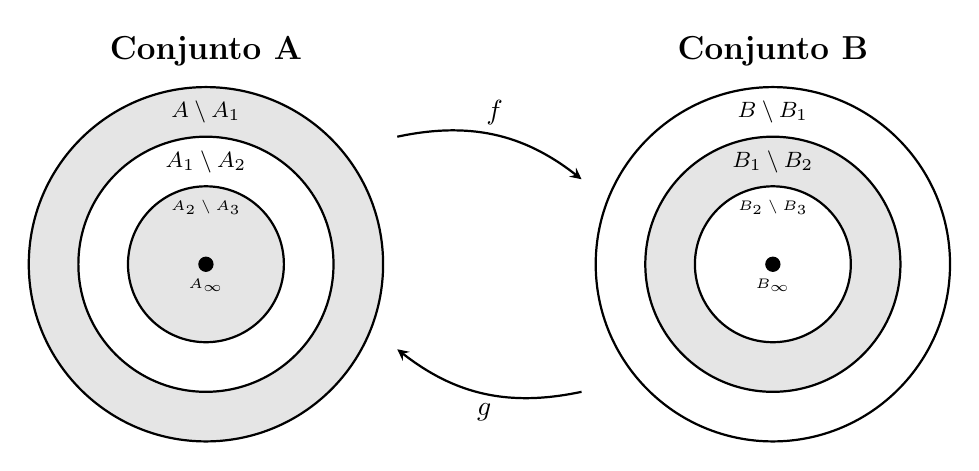
\begin{tikzpicture}[scale=0.9, >=stealth]
    % === CONJUNTO A (Izquierda) ===
    % Patrón: GRIS - BLANCO - GRIS
    \node at (-4, 3.0) {\large \textbf{Conjunto A}};

    % 1. Capa Exterior (Gris) - Se va a ir a B
    \draw[thick, fill=gray!20] (-4,0) circle (2.5cm);
    \node at (-4, 2.15) {\footnotesize $A \setminus A_1$}; 

    % 2. Capa Media (Blanca) - Viene de B
    \draw[thick, fill=white] (-4,0) circle (1.8cm);
    \node at (-4, 1.45) {\footnotesize $A_1 \setminus A_2$}; 

    % 3. Capa Interna (Gris) - Se va a ir a B
    \draw[thick, fill=gray!20] (-4,0) circle (1.1cm);
    \node at (-4, 0.8) {\tiny $A_2 \setminus A_3$}; 
    
    % Núcleo
    \draw[fill=black] (-4,0) circle (0.1cm);
    \node at (-4, -0.3) {\tiny $A_\infty$};

    % === CONJUNTO B (Derecha) ===
    % Patrón INVERTIDO: BLANCO - GRIS - BLANCO
    \node at (4, 3.0) {\large \textbf{Conjunto B}};

    % 1. Capa Exterior (Blanca) - Se va a ir a A
    \draw[thick, fill=white] (4,0) circle (2.5cm);
    \node at (4, 2.15) {\footnotesize $B \setminus B_1$};

    % 2. Capa Media (Gris) - Viene de A
    \draw[thick, fill=gray!20] (4,0) circle (1.8cm);
    \node at (4, 1.45) {\footnotesize $B_1 \setminus B_2$};

    % 3. Capa Interna (Blanca) - Se va a ir a A
    \draw[thick, fill=white] (4,0) circle (1.1cm);
    \node at (4, 0.8) {\tiny $B_2 \setminus B_3$};

    % Núcleo
    \draw[fill=black] (4,0) circle (0.1cm);
    \node at (4, -0.3) {\tiny $B_\infty$};
    
    % Flecha f: Sale de GRIS (A) -> Entra a GRIS (B)
    \draw[->, thick] (-1.3, 1.8) to[bend left=25] node[midway, above] {$f$} (1.3, 1.2);
    
    % Flecha g: Sale de BLANCO (B) -> Entra a BLANCO (A)
    \draw[->, thick] (1.3, -1.8) to[bend left=25] node[midway, below] {$g$} (-1.3, -1.2);

\end{tikzpicture}
\end{figure}

\begin{proof}
Se define recursivamente
\begin{align*}
    A_1 &= g(B) & B_1 &= f(A) \\
    A_2 &= g(B_1) & B_2 &= f(A_1) \\
    &\vdots & &\vdots \\
    A_{k+1} &= g(B_k) & B_{k+1} &= f(A_k) \\
    A_\infty &= \bigcap_{k=1}^{\infty} A_k \quad & \quad B_\infty &= \bigcap_{k=1}^{\infty} B_k.
\end{align*}

$A$ y $B$ se escriben como uniones disjuntas de las capas y los núcleos, y $h$ actúa de
manera distinta en cada parte.

\[
\setlength{\arraycolsep}{6pt}
\begin{array}{rcccl}
    % --- FILA DEL CONJUNTO A ---
    A \; = & 
    \underbrace{\left[ (A \setminus A_1) \cup (A_2 \setminus A_3) \cup \dots \right]}_{\text{Capas
    pares de A}} & 
    \cup & 
    \underbrace{\left[ (A_1 \setminus A_2) \cup (A_3 \setminus A_4) \cup \dots \right]}_{\text{Capas
    impares de A}} & 
    \cup \underbrace{A_\infty}_{\text{Núcleo de A}} \\
    
    % --- FILA DE FLECHAS ---
    & 
    \Bigg\downarrow f \quad \Bigg\uparrow f^{-1} & 
    & 
    \Bigg\downarrow g^{-1} \quad \Bigg\uparrow g &
    
    \hspace{0.5cm} \Bigg\downarrow f \quad \Bigg\uparrow f^{-1} \\
    
    % --- FILA DEL CONJUNTO B ---
    B \; = & 
    \underbrace{\left[ (B_1 \setminus B_2) \cup (B_3 \setminus B_4) \cup \dots \right]}_{\text{Capas
    Impares de B}} & 
    \cup & 
    \underbrace{\left[ (B \setminus B_1) \cup (B_2 \setminus B_3) \cup \dots \right]}_{\text{Capas
    Pares de B}} & 
    \cup \underbrace{B_\infty}_{\text{Núcleo de B}} \\
\end{array}
\]

Se define $h: A \to B$ por casos:
$$
h(x) = \begin{cases}
    f(x) & \text{si } x \in A_k \setminus A_{k+1} \text{ con } k \text{ par,} \\
    g^{-1}(x) & \text{si } x \in A_k \setminus A_{k+1} \text{ con } k \text{ impar,} \\
    f(x) & \text{si } x \in A_\infty.
\end{cases}
$$

La inyectividad se sigue de que $f$ y $g$ lo son. Resta ver la sobreyectividad en cada parte.

\begin{enumerate}
    \item \textit{Anillos pares.} La restricción
    $f: (A_{2k} \setminus A_{2k+1}) \to (B_{2k+1} \setminus B_{2k+2})$ es sobre. Si
    $y \in B_{2k+1} \setminus B_{2k+2}$, como $B_{2k+1} = f(A_{2k})$ existe $x \in A_{2k}$ con
    $f(x) = y$. Si fuera $x \in A_{2k+1}$, entonces $y = f(x) \in f(A_{2k+1}) = B_{2k+2}$, absurdo.
    Así que $x \in A_{2k} \setminus A_{2k+1}$.

    \item \textit{Anillos impares.} Ahora la restricción
    $g^{-1}: (A_{2k-1} \setminus A_{2k}) \to (B_{2k-2} \setminus B_{2k-1})$. Equivale a ver que
    $$ g: (B_{2k-2} \setminus B_{2k-1}) \to (A_{2k-1} \setminus A_{2k}) $$
    es biyección. Se toma $x \in A_{2k-1} \setminus A_{2k}$; como $A_{2k-1} = g(B_{2k-2})$, hay
    $y \in B_{2k-2}$ con $g(y) = x$. Si $y \in B_{2k-1}$, entonces
    $x = g(y) \in g(B_{2k-1}) = A_{2k}$, contradicción.

    \item \textit{El núcleo.} Para $f: A_\infty \to B_\infty$, dado $z \in B_\infty$ se tiene
    $z \in B_{k+1} = f(A_k)$ para todo $k$. Hay entonces $x_k \in A_k$ con $f(x_k) = z$; por
    inyectividad de $f$ es \emph{el mismo} $x$ para todos los $k$. Luego
    $x \in \bigcap A_k = A_\infty$ y $z = f(x)$.
\end{enumerate}
$h$ es biyección y por lo tanto $A \sim B$.
\end{proof}

\subsection{Álgebra de Conjuntos Numerables}

\begin{teorema}{Producto Cartesiano}{prod_cart}
El producto cartesiano finito de numerables es numerable. En particular,
$\mathbb{N} \times \mathbb{N} \sim \mathbb{N}$.
\end{teorema}
\begin{proof}
Por inducción sobre la cantidad $k$ de factores. El caso $k=1$ es la hipótesis: un único
factor, ya numerable. Para el paso inductivo, por asociatividad
$$ A_1 \times \cdots \times A_n \times A_{n+1} = (A_1 \times \cdots \times A_n) \times A_{n+1} = P_n
\times A_{n+1}, $$
y todo se reduce a ver que el producto de dos numerables es numerable. Y eso a su vez se obtiene
viendo que $\mathbb{N} \times \mathbb{N} \sim \mathbb{N}$: la función $f(n,m) = 2^n 3^m$ es
inyectiva por el Teorema Fundamental de la Aritmética.
\end{proof}

\begin{teorema}{Unión Numerable}{union_num}
$$ A = \bigcup_{n \in \mathbb{N}} A_n, \quad \text{con } A_n \text{ numerable} \implies A
\text{ es numerable.} $$
\end{teorema}
\begin{proof}
Si los $A_n$ no son disjuntos, un elemento puede quedar contado varias veces, lo que impide construir
una inyección directa. Se reemplaza $(A_n)$ por una familia disjunta con la misma unión:
$$ A'_1 = A_1, \qquad A'_n = A_n \setminus \bigcup_{k=1}^{n-1} A_k \quad (n > 1). $$
Cada $A'_n \subseteq A_n$ es numerable, los $A'_n$ son disjuntos dos a dos, y
$\bigcup A'_n = \bigcup A_n$.

Así que se tienen inyecciones $g_n: A'_n \to \mathbb{N}$. Se define
$H: A \to \mathbb{N} \times \mathbb{N}$: dado $x \in A$, hay un único $n$ con $x \in A'_n$ (porque
son disjuntos), y se pone $H(x) = (n, g_n(x))$. $H$ es inyectiva. Como
$\mathbb{N} \times \mathbb{N} \sim \mathbb{N}$, $A$ es numerable.
\end{proof}

\begin{teorema}{Racionales}{racionales}
$\mathbb{Q}$ es numerable.
\end{teorema}
\begin{proof}
Mediante la asignación $p/q \mapsto (p, q)$ (con $q \in \mathbb{N}$, $p \in \mathbb{Z}$ y $\mathrm{mcd}(p,q)=1$)
se inyecta $\mathbb{Q}$ en $\mathbb{Z} \times \mathbb{N}$, que es numerable.
\end{proof}

\subsection{Conjuntos No Numerables}

\begin{teorema}{No Numerabilidad del Intervalo}{intervalo_no_num}
El intervalo $(0,1)$ no es numerable.
\end{teorema}

\begin{proof}
Por el argumento diagonal de Cantor. Si fuera numerable, se podrían listar sus elementos:
\begin{align*}
y_1 &= 0,d_{11}d_{12}d_{13}\dots \\
y_2 &= 0,d_{21}d_{22}d_{23}\dots \\
\vdots & \\
y_k &= 0,d_{k1}d_{k2}d_{k3}\dots
\end{align*}
Se construye $z = 0,z_1z_2z_3\dots$ con $z_k \ne d_{kk}$ (por ejemplo, $z_k = 2$ si $d_{kk}=1$ y
$z_k = 1$ si no). Entonces $z$ difiere de cada $y_k$ en la $k$-ésima cifra, de modo que
$z \notin \{y_k\}$, contra la suposición de que la lista cubría $(0,1)$.
\end{proof}

\begin{corolario}{Reales}{reales}
$\mathbb{R}$ no es numerable.
\end{corolario}

\begin{proof}
Primero, $(0,1) \sim (a,b)$ vía la lineal $t \mapsto a + t(b-a)$. Segundo,
$\mathbb{R} \sim (-\pi/2, \pi/2)$ vía $\arctan$. Composición da $\mathbb{R} \sim (0,1)$, que no
es numerable.
\end{proof}

\subsection*{Comentario sobre la notación y el orden de cardinales}

\begin{lema}[Inyectividad y Sobreyectividad por Composición]\label{lema:iny_sob_comp}
Si $f: A \to B$, $g: B \to A$ y $g \circ f = \mathrm{id}_A$, entonces $f$ es inyectiva y $g$ es
sobreyectiva.
\end{lema}

\begin{proof}
\textit{$f$ inyectiva.} Si $f(x_1) = f(x_2)$, aplicando $g$ queda $x_1 = g(f(x_1)) = g(f(x_2)) = x_2$.

\textit{$g$ sobreyectiva.} Dado $a \in A$, se toma $b = f(a)$ y $g(b) = a$.
\end{proof}

Con esto se define el orden de cardinales:

\begin{definicion}{Desigualdad de Cardinales}{}
$\#A \le \#B$ si existe una inyección $f: A \to B$.
\end{definicion}

Hay una formulación equivalente con sobreyecciones en el otro sentido:

\begin{proposicion}{Equivalencia de $\#A \le \#B$}{}
Si $A \ne \emptyset$, $\#A \le \#B$ si y solo si existe una sobreyección $g: B \to A$.
\end{proposicion}

\begin{proof}
Se prueban las dos implicaciones.

\textit{($\Rightarrow$).} Sea $f: A \to B$ inyectiva. Se define $g: B \to A$: para $b \in f(A)$ se
toma $g(b)$ el único $a$ con $f(a) = b$, y para $b \notin f(A)$ se asigna un $a_0 \in A$
fijo (aquí se usa $A \ne \emptyset$). Así $g \circ f = \mathrm{id}_A$ y, por el
Lema~\ref{lema:iny_sob_comp}, $g$ es sobreyectiva.

\textit{($\Leftarrow$).} Sea $g$ sobreyectiva. Por el axioma de elección, para cada $a$ se elige
$b_a \in g^{-1}(\{a\})$ y se define $f(a) = b_a$. Entonces $g \circ f = \mathrm{id}_A$ y $f$ es
inyectiva.
\end{proof}


\subsection{Teorema de Cantor (Conjunto Potencia)}

\begin{teorema}{Teorema de Cantor}{potencia}
$|A| < |\mathcal{P}(A)|$ para todo conjunto $A$.
\end{teorema}

\begin{proof}
$|A| \le |\mathcal{P}(A)|$ porque $a \mapsto \{a\}$ es inyectiva. Para ver que no hay sobreyección
$h: A \to \mathcal{P}(A)$, razónese por el absurdo (argumento diagonal): si $h$ fuera sobre, con el
conjunto diagonal
$$ B = \{ x \in A : x \notin h(x) \} \in \mathcal{P}(A) $$
habría $b \in A$ con $h(b) = B$. Pero
\begin{itemize}
    \item $b \in B \implies b \notin h(b) = B$,
    \item $b \notin B \implies b \in h(b) = B$.
\end{itemize}
Ambas son absurdas, de modo que no existe tal $h$.
\end{proof}

\newpage

\subsection{Ejercicios resueltos}

\subsection*{Ejercicio 1}

Dados $A$ y $B$ subconjuntos de $X$.

\begin{proposicion}{Ejercicio 1.i}{ej1_i}
Probar que $A \subset B \iff B^c \subset A^c$.
\end{proposicion}

\begin{proof}
Se prueban las dos implicaciones.

\textit{($\Rightarrow$).} Supóngase que $A \subset B$; hay que ver que $B^c \subset A^c$.
\begin{itemize}
    \item Sea $x \in B^c$, es decir, $x \notin B$.
    \item Por hipótesis $A \subset B$, de modo que si $x$ estuviera en $A$ estaría en $B$.
    \item Como $x \notin B$, por contrarrecíproco se concluye $x \notin A$.
    \item Si $x \notin A$, entonces $x \in A^c$.
\end{itemize}

\textit{($\Leftarrow$).} Supóngase que $B^c \subset A^c$; hay que ver que $A \subset B$.
\begin{itemize}
    \item Sea $x \in A$, es decir, $x \notin A^c$.
    \item Por hipótesis ($B^c \subset A^c$), si $x$ perteneciera a $B^c$ pertenecería a $A^c$.
    \item Como $x \notin A^c$, no puede ser $x \in B^c$.
    \item Por lo tanto $x \notin B^c$, lo que implica $x \in B$.
\end{itemize}
\end{proof}

\begin{proposicion}{Ejercicio 1.ii}{ej1_ii}
Probar que $B - \bigcup_{i} A_i = \bigcap_{i} (B - A_i)$.
\end{proposicion}

\begin{proof}
Se prueba la doble inclusión.

\textit{($\subseteq$).} Sea $x \in B - \bigcup_{i} A_i$.
\begin{itemize}
    \item Por definición de diferencia, $x \in B$ \emph{y} $x \notin \bigcup_{i} A_i$.
    \item Que $x$ no esté en la unión significa que no pertenece a ninguno de los $A_i$; es decir,
    $\forall i, x \notin A_i$.
    \item Como $x \in B$ y además $\forall i, x \notin A_i$, se tiene
    $\forall i, (x \in B \land x \notin A_i)$.
    \item Esto equivale a $\forall i, x \in (B - A_i)$.
    \item Por definición de intersección generalizada, $x \in \bigcap_{i} (B - A_i)$.
\end{itemize}

\textit{($\supseteq$).} Sea $x \in \bigcap_{i} (B - A_i)$.
\begin{itemize}
    \item Por definición de intersección, $\forall i, x \in (B - A_i)$.
    \item Es decir, para todo $i$: $x \in B$ \emph{y} $x \notin A_i$.
    \item De aquí se obtienen dos cosas:
    \begin{enumerate}
        \item $x \in B$ (común a todos).
        \item $\forall i, x \notin A_i$.
    \end{enumerate}
    \item La segunda condición implica que no hay índice con $x \in A_i$; por lo tanto
    $x \notin \bigcup_{i} A_i$.
    \item Al juntar $x \in B$ y $x \notin \bigcup_{i} A_i$, se obtiene $x \in B - \bigcup_{i} A_i$.
\end{itemize}
\end{proof}

\begin{proposicion}{Ejercicio 1.iii}{ej1_iii}
Probar que $B - \bigcap_{i} A_i = \bigcup_{i} (B - A_i)$.
\end{proposicion}

\begin{proof}
Se prueba la doble inclusión.

\textit{($\subseteq$).} Sea $x \in B - \bigcap_{i} A_i$.
\begin{itemize}
    \item Entonces $x \in B$ \emph{y} $x \notin \bigcap_{i} A_i$.
    \item Negar que $x$ esté en la intersección significa que falla en al menos uno: existe algún
    índice $k$ con $x \notin A_k$.
    \item Como $x \in B$ y para ese $k$ se tiene $x \notin A_k$, entonces $x \in (B - A_k)$.
    \item Como $x$ pertenece a uno de los conjuntos de la familia, pertenece a la unión.
\end{itemize}

\textit{($\supseteq$).} Sea $x \in \bigcup_{i} (B - A_i)$.
\begin{itemize}
    \item Por definición de unión, existe algún índice $k$ con $x \in (B - A_k)$.
    \item Es decir, $x \in B$ y $x \notin A_k$.
    \item Como $x \notin A_k$, $x$ no puede estar en la intersección de todos los $A_i$ (pues $x \notin A_k$). Por tanto $x \notin \bigcap_{i} A_i$.
    \item Al tener $x \in B$ y $x \notin \bigcap_{i} A_i$, se concluye $x \in B - \bigcap_{i} A_i$.
\end{itemize}
\end{proof}

\begin{proposicion}{Ejercicio 1.iv}{ej1_iv}
Probar que $\bigcup_{i} (A_i \cap B) = (\bigcup_{i} A_i) \cap B$.
\end{proposicion}

\begin{proof}
Se prueba la doble inclusión.

\textit{($\subseteq$).} Sea $x \in \bigcup_{i} (A_i \cap B)$.
\begin{itemize}
    \item Existe algún índice $k$ con $x \in (A_k \cap B)$.
    \item Es decir, $x \in A_k$ y $x \in B$.
    \item Como $x \in A_k$, entonces $x \in \bigcup_{i} A_i$ (basta estar en uno).
    \item Como $x \in \bigcup_{i} A_i$ y además $x \in B$, entonces $x \in (\bigcup_{i} A_i) \cap B$.
\end{itemize}

\textit{($\supseteq$).} Sea $x \in (\bigcup_{i} A_i) \cap B$.
\begin{itemize}
    \item Entonces $x \in \bigcup_{i} A_i$ y $x \in B$.
    \item Por estar en la unión, existe un índice $k$ con $x \in A_k$.
    \item Como $x \in A_k$ y $x \in B$, entonces $x \in (A_k \cap B)$.
    \item Al pertenecer a uno de los términos $(A_k \cap B)$, pertenece a la unión.
\end{itemize}
\end{proof}

\subsection*{Ejercicio 2}

Dada una sucesión $(A_{n})_{n\in\mathbb{N}}$ de conjuntos, y $A=\bigcup_{n}A_{n}$, hallar una
sucesión $(B_{n})_{n\in\mathbb{N}}$ de conjuntos disjuntos tales que $A=\bigcup_{n}B_{n}$.

\begin{proof}
Se define la sucesión $(B_n)$ de manera recursiva:
$$ B_1 = A_1 $$
$$ B_n = A_n \setminus \left( \bigcup_{k=1}^{n-1} A_k \right) \quad \text{para } n > 1 $$

Hay que probar dos cosas: que son disjuntos y que su unión es $A$.

\textit{Disjuntos.} Sean $n, m \in \mathbb{N}$ con $n \neq m$; sin pérdida de generalidad, $m < n$.
Por definición,
$$ B_n = A_n \setminus (A_1 \cup \dots \cup A_m \cup \dots \cup A_{n-1}), $$
de modo que $B_n$ no tiene ningún elemento de $A_m$, es decir, $B_n \cap A_m = \emptyset$. Como
$B_m \subseteq A_m$ por construcción, se tiene $B_n \cap B_m = \emptyset$.

\textit{Igualdad de las uniones.} Se prueba la doble inclusión.

$(\subseteq)$ Como $B_n \subseteq A_n$ para todo $n$,
$$ \bigcup_{n=1}^{\infty} B_n \subseteq \bigcup_{n=1}^{\infty} A_n = A. $$

$(\supseteq)$ Sea $x \in A = \bigcup_{n=1}^{\infty} A_n$; entonces $x$ pertenece al menos a uno de los
$A_n$. Sea $k$ el menor índice con $x \in A_k$. Esto implica $x \in A_k$ y $x \notin A_j$ para todo
$j < k$ (si no, $k$ no sería el menor). Luego $x$ no pertenece a la unión de los anteriores:
$$ x \notin \bigcup_{j=1}^{k-1} A_j, $$
y por definición de $B_k$ se tiene $x \in A_k \setminus \bigcup_{j=1}^{k-1} A_j$, es decir,
$x \in B_k$. Por lo tanto $x \in \bigcup_{n=1}^{\infty} B_n$.

Finalmente, $A=\bigcup_{n}B_{n}$.
\end{proof}

\subsection*{Ejercicio 3}

Dada una función $f:X\longrightarrow Y$ y subconjuntos $A, B$ de $X$ y $C, D$ de $Y$.

\begin{proposicion}{3.i}{ej3_i}
$f(A\cup B)=f(A)\cup f(B)$
\end{proposicion}

\begin{proof}
Se prueba la doble inclusión.

\textit{($\subseteq$).} Sea $y \in f(A \cup B)$. Por definición de imagen directa, existe
$x \in A \cup B$ con $f(x) = y$. Como $x \in A$ o $x \in B$:
\begin{itemize}
    \item si $x \in A$, entonces $f(x) \in f(A)$, luego $y \in f(A)$;
    \item si $x \in B$, entonces $f(x) \in f(B)$, luego $y \in f(B)$.
\end{itemize}
En cualquier caso, $y \in f(A) \cup f(B)$.

\textit{($\supseteq$).} Sea $y \in f(A) \cup f(B)$, es decir, $y \in f(A)$ o $y \in f(B)$.
\begin{itemize}
    \item Si $y \in f(A)$, existe $x \in A$ con $f(x) = y$. Como $A \subset A \cup B$, entonces
    $x \in A \cup B$, por lo que $y \in f(A \cup B)$.
    \item Análogamente, si $y \in f(B)$, existe $x \in B$ con $f(x) = y$, y $y \in f(A \cup B)$.
\end{itemize}
\end{proof}

\begin{proposicion}{3.ii}{ej3_ii}
$f(A\cap B)\subset f(A)\cap f(B)$. ¿Vale la igualdad?
\end{proposicion}

\begin{proof}
Sea $y \in f(A \cap B)$. Existe $x \in A \cap B$ con $f(x) = y$. Como $x \in A$ y $x \in B$, se tiene
$f(x) \in f(A)$ y $f(x) \in f(B)$, luego $y \in f(A) \cap f(B)$.
\end{proof}

La igualdad no vale en general. Como contraejemplo, sea $f: \mathbb{R} \to \mathbb{R}$, $f(x) = x^2$,
y sean $A = [-1, 0]$, $B = [0, 1]$. Entonces $A \cap B = \{0\}$, de modo que $f(A \cap B) = \{0\}$;
en cambio $f(A) = [0, 1] = f(B)$, de modo que $f(A) \cap f(B) = [0, 1] \neq \{0\}$.

\begin{proposicion}{3.iii}{ej3_iii}
$f^{-1}(C\cup D)=f^{-1}(C)\cup f^{-1}(D)$
\end{proposicion}

\begin{proof}
Sea $x$ un elemento cualquiera:
\begin{align*}
x \in f^{-1}(C \cup D) &\iff f(x) \in C \cup D \\
&\iff f(x) \in C \lor f(x) \in D \\
&\iff x \in f^{-1}(C) \lor x \in f^{-1}(D) \\
&\iff x \in f^{-1}(C) \cup f^{-1}(D). \qedhere
\end{align*}
\end{proof}

\begin{proposicion}{3.iv}{ej3_iv}
$f^{-1}(C\cap D)=f^{-1}(C)\cap f^{-1}(D)$
\end{proposicion}

\begin{proof}
Sea $x$ un elemento cualquiera:
\begin{align*}
x \in f^{-1}(C \cap D) &\iff f(x) \in C \cap D \\
&\iff f(x) \in C \land f(x) \in D \\
&\iff x \in f^{-1}(C) \land x \in f^{-1}(D) \\
&\iff x \in f^{-1}(C) \cap f^{-1}(D). \qedhere
\end{align*}
\end{proof}

\begin{proposicion}{3.v}{ej3_v}
$A\subset f^{-1}(f(A))$. ¿Vale la igualdad?
\end{proposicion}

\begin{proof}
Sea $x \in A$. Aplicando $f$, $f(x) \in f(A)$. Por definición de preimagen, $f^{-1}(f(A))$ contiene
a todos los elementos cuya imagen está en $f(A)$; como $f(x) \in f(A)$, entonces $x \in f^{-1}(f(A))$.
\end{proof}

La igualdad no vale en general (solo si $f$ es inyectiva). Como contraejemplo, sea $f(x) = x^2$ y
$A = \{1\}$: entonces $f(A) = \{1\}$ y $f^{-1}(f(A)) = f^{-1}(\{1\}) = \{-1, 1\}$, con
$\{1\} \subsetneq \{-1, 1\}$.

\begin{proposicion}{3.vi}{ej3_vi}
$f(f^{-1}(C))\subset C$. ¿Vale la igualdad?
\end{proposicion}

\begin{proof}
Sea $y \in f(f^{-1}(C))$. Por definición de imagen directa, existe $x \in f^{-1}(C)$ con $f(x) = y$;
y por definición de preimagen, $x \in f^{-1}(C)$ implica $f(x) \in C$. Como $f(x) = y$, se concluye
$y \in C$.
\end{proof}

La igualdad no vale en general (solo si $f$ es sobreyectiva o si $C \subset \operatorname{Im}(f)$).
Como contraejemplo, sea $f(x) = e^x$ de $\mathbb{R}$ en $\mathbb{R}$ y $C = \mathbb{R}$: entonces
$f^{-1}(C) = \mathbb{R}$ y $f(f^{-1}(C)) = f(\mathbb{R}) = (0, \infty)$, con
$(0, \infty) \subsetneq \mathbb{R}$.

\begin{proposicion}{3.vii}{ej3_vii}
$f^{-1}(D^c) = (f^{-1}(D))^c$
\end{proposicion}

\begin{proof}
Sea $x$ un elemento cualquiera:
\begin{align*}
x \in f^{-1}(D^c) &\iff f(x) \in D^c \\
&\iff f(x) \notin D \\
&\iff \neg (f(x) \in D) \\
&\iff \neg (x \in f^{-1}(D)) \\
&\iff x \notin f^{-1}(D) \\
&\iff x \in (f^{-1}(D))^c. \qedhere
\end{align*}
\end{proof}

\subsection*{Ejercicio 4}

\begin{proposicion}{Relación $\to$ Partición}{ej4_rel_part}
Sea $X$ un conjunto y $\sim$ una relación de equivalencia sobre $X$.
El conjunto de clases de equivalencia (conjunto cociente) $X/\sim = \{ [x] : x \in X \}$ forma una
partición de $X$.
\end{proposicion}

\begin{proof}
Una familia de conjuntos es una partición si cumple tres condiciones.

\textit{Las clases no son vacías.} Sea $[x]$ una clase cualquiera. Por reflexividad, $x \sim x$, y
por definición de clase ($[x] = \{y \in X : y \sim x\}$) esto da $x \in [x]$. Luego
$[x] \neq \emptyset$.

\textit{La unión cubre $X$.} La unión de subconjuntos de $X$ está contenida en $X$. Para la otra
inclusión, sea $x \in X$; como $x \in [x]$, el elemento $x$ pertenece a la unión de todas las clases.
Por lo tanto
$$ X = \bigcup_{x \in X} [x]. $$

\textit{Son disjuntas dos a dos.} Sean $[x]$ y $[y]$ dos clases; hay que ver que son disjuntas o
idénticas. Supóngase que no son disjuntas, es decir, existe $z \in [x] \cap [y]$.
\begin{itemize}
    \item $z \in [x] \implies z \sim x \implies x \sim z$.
    \item $z \in [y] \implies z \sim y$.
    \item Por transitividad, $x \sim y$.
\end{itemize}
Ahora se ve que $[x] = [y]$. Sea $w \in [x]$, esto es $w \sim x$; como $w \sim x$ y $x \sim y$, por
transitividad $w \sim y$, luego $w \in [y]$. Esto prueba $[x] \subseteq [y]$, y por simetría vale la
inclusión opuesta. Así, dos clases que comparten un elemento son iguales; si son distintas, su
intersección es vacía.
\end{proof}

\begin{proposicion}{Partición $\to$ Relación}{ej4_part_rel}
Sea $P = \{A_i\}_{i \in I}$ una partición de un conjunto $X$.
La relación definida por $x \sim y \iff \exists k \in I$ tal que $x \in A_k \land y \in A_k$ es de
equivalencia.
\end{proposicion}

\begin{proof}
Se verifican las tres propiedades.

\textit{Reflexividad.} Sea $x \in X$. Como $P$ es una partición, la unión de los $A_i$ cubre $X$, de modo
que existe un índice $k$ con $x \in A_k$. Entonces $x$ y $x$ están en el mismo $A_k$, luego
$x \sim x$.

\textit{Simetría.} Supóngase $x \sim y$, es decir, existe $k$ con $x, y \in A_k$. Entonces también
$y, x \in A_k$, luego $y \sim x$.

\textit{Transitividad.} Supóngase $x \sim y$ y $y \sim z$.
\begin{itemize}
    \item $x \sim y \implies \exists k$ con $x, y \in A_k$.
    \item $y \sim z \implies \exists j$ con $y, z \in A_j$.
\end{itemize}
El elemento $y$ pertenece tanto a $A_k$ como a $A_j$. Como los elementos de $P$ son disjuntos dos a
dos, la única forma de que $A_k \cap A_j \neq \emptyset$ es $A_k = A_j$. Luego $x$ y $z$ están en el
mismo conjunto, y $x \sim z$.
\end{proof}

\subsection*{Ejercicio 5}

Este ejercicio ya fue resuelto.

\subsection*{Ejercicio 6}

El ejercicio propone usar el principio de inducción completa.
Dada una propiedad $P(n)$, se define el conjunto de verdad
$S = \{n \in \mathbb{N} : P(n) \text{ es verdadera}\}$.
Si se prueba que $1 \in S$ y que el cumplimiento de la propiedad para todos los anteriores implica el
cumplimiento para el siguiente, entonces $S = \mathbb{N}$ (la fórmula vale para todos).

\begin{proposicion}{6.i}{ej6_i}
$$ \sum_{k=1}^{n}k=\frac{n(n+1)}{2} $$
\end{proposicion}

\begin{proof}
Por inducción sobre $n$. Sea $S = \{ n \in \mathbb{N} : \sum_{k=1}^{n}k=\frac{n(n+1)}{2} \}$.

\textit{Caso base ($n=1$).} El lado izquierdo es $\sum_{k=1}^{1} k = 1$ y el derecho es
$\frac{1(1+1)}{2} = \frac{2}{2} = 1$. Como coinciden, $1 \in S$.

\textit{Paso inductivo.} Supóngase que $n \in S$; hay que probar que
$\sum_{k=1}^{n+1}k = \frac{(n+1)(n+2)}{2}$. Partiendo de la suma hasta $n+1$,
$$ \sum_{k=1}^{n+1}k = \left( \sum_{k=1}^{n}k \right) + (n+1). $$
Usando la hipótesis inductiva en la suma hasta $n$,
$$ = \frac{n(n+1)}{2} + (n+1). $$
Sacando factor común $(n+1)$ y operando,
$$ = (n+1) \left( \frac{n}{2} + 1 \right) = (n+1) \left( \frac{n+2}{2} \right) = \frac{(n+1)(n+2)}{2}. $$
Luego $n+1 \in S$, y por inducción $S = \mathbb{N}$.
\end{proof}

\begin{proposicion}{6.ii}{ej6_ii}
$$ \sum_{k=0}^{n}r^{k}=\frac{r^{n+1}-1}{r-1} \quad (r \neq 1) $$
\end{proposicion}

\begin{proof}
Por inducción sobre $n$. Sea $S = \{ n \in \mathbb{N} : \sum_{k=0}^{n}r^{k}=\frac{r^{n+1}-1}{r-1} \}$.

\textit{Caso base ($n=1$).} El lado izquierdo es $\sum_{k=0}^{1} r^k = r^0 + r^1 = 1 + r$ y el
derecho $\frac{r^{1+1}-1}{r-1} = \frac{r^2-1}{r-1} = \frac{(r-1)(r+1)}{r-1} = r+1$. Como coinciden,
$1 \in S$.

\textit{Paso inductivo.} Supóngase que $n \in S$; hay que probar que la suma hasta $n+1$ da
$\frac{r^{n+2}-1}{r-1}$. Partiendo de la suma,
$$ \sum_{k=0}^{n+1} r^k = \left( \sum_{k=0}^{n} r^k \right) + r^{n+1}, $$
usando la hipótesis inductiva,
$$ = \frac{r^{n+1}-1}{r-1} + r^{n+1}, $$
y sacando denominador común, distribuyendo y cancelando $r^{n+1}$ con $-r^{n+1}$,
$$ = \frac{r^{n+1}-1 + r^{n+1}(r-1)}{r-1} = \frac{r^{n+1} - 1 + r^{n+2} - r^{n+1}}{r-1}
= \frac{r^{n+2} - 1}{r-1}. $$
Esta es la fórmula en $n+1$, luego $n+1 \in S$ y por inducción $S = \mathbb{N}$.
\end{proof}

\subsection*{Ejercicio 7}

Probar el Principio de Buena Ordenación: Todo subconjunto no vacío de $\mathbb{N}$ tiene mínimo.

\begin{proof}
Razónese por el absurdo. Sea $A \subseteq \mathbb{N}$ no vacío y supóngase que $A$ no tiene mínimo.
Se define el conjunto de los naturales estrictamente menores que cualquier elemento de $A$:
$$ S = \{ n \in \mathbb{N} : \forall a \in A,\ n < a \}. $$
Se prueba por inducción que $S = \mathbb{N}$.

\textit{Caso base.} Como $1$ es el menor natural ($1 \le x$ para todo $x \in \mathbb{N}$), si fuera
$1 \in A$ entonces $1$ sería el mínimo de $A$. Como $A$ no tiene mínimo, $1 \notin A$; luego
$\{1\} \cap A = \emptyset$, lo que da $1 \in S$.

\textit{Paso inductivo.} Supóngase $n \in S$, es decir, $\{1, 2, \dots, n\} \cap A = \emptyset$. Si
fuera $n+1 \in A$, como $1, \dots, n$ no están en $A$, entonces $n+1$ sería el mínimo de $A$, que no
existe. Por lo tanto $n+1 \notin A$, de modo que $\{1, 2, \dots, n, n+1\} \cap A = \emptyset$ y
$n+1 \in S$.

Por inducción, $S = \mathbb{N}$, es decir, $n \notin A$ para todo natural $n$, y en consecuencia
$A = \emptyset$. Esto contradice que $A$ sea no vacío. La contradicción proviene de suponer que $A$
no tiene mínimo; luego $A$ tiene mínimo.
\end{proof}

\subsection*{Ejercicio 8}

Hallar el cardinal de los siguientes conjuntos.

\begin{itemize}
    \item Conjunto: $\mathbb{Z}_{\ge 3} = \{ n \in \mathbb{Z} : n \ge 3 \}$.
    Cardinal: $\aleph_0$.
    \\ Es un subconjunto infinito de un conjunto numerable ($\mathbb{Z}$), por lo tanto es
    numerable. Se establece la biyección explícita $f: \mathbb{N} \to \mathbb{Z}_{\ge 3}$ dada
    por $f(n) = n + 2$.

    \item Conjunto: $5\mathbb{Z} = \{ 5k : k \in \mathbb{Z} \}$.
    Cardinal: $\aleph_0$.
    \\ Se define la función $f: \mathbb{Z} \to 5\mathbb{Z}$ como $f(k) = 5k$, que es biyectiva
    (inyectiva porque $5k_1=5k_2 \implies k_1=k_2$ y sobreyectiva por definición). Como
    $\mathbb{Z} \sim \mathbb{N}$, entonces $5\mathbb{Z} \sim \mathbb{N}$.

    \item Conjunto: $\mathbb{Z} \times \mathbb{N}$.
    Cardinal: $\aleph_0$.
    \\ Tanto $\mathbb{Z}$ como $\mathbb{N}$ son numerables. Por el Teorema \ref{teo:prod_cart}, el
    producto cartesiano finito de conjuntos numerables es numerable.

    \item Conjunto: $\mathbb{R} - \mathbb{Q}$.
    Cardinal: $c$.
    \\ Se tiene $\mathbb{R} = (\mathbb{R} - \mathbb{Q}) \cup \mathbb{Q}$. Por el absurdo: si los irracionales fueran
    numerables, como $\mathbb{Q}$ es numerable, $\mathbb{R}$ sería unión de dos numerables, y por
    tanto numerable; esto contradice la no numerabilidad de los reales. Luego
    $\mathbb{R} - \mathbb{Q}$ es no numerable.

    \item Conjunto: $(-1, 1) \cap \mathbb{Q}$.
    Cardinal: $\aleph_0$.
    \\ Es un subconjunto de $\mathbb{Q}$, y todo subconjunto de un conjunto numerable es a lo sumo
    numerable.
\end{itemize}

\subsection*{Ejercicio 9}

Probar que el conjunto de números primos es numerable.

\begin{proof}
Sea $P$ el conjunto de los números primos. Como $P \subset \mathbb{N}$, basta ver que es infinito.
Razónese por el absurdo: supóngase que hay una cantidad finita de primos $p_1, p_2, \dots, p_n$, y
considérese
$$ Q = (p_1 \cdot p_2 \cdot \dots \cdot p_n) + 1. $$
El número $Q$ tiene algún divisor primo $q$.
\begin{itemize}
    \item Si $q$ fuera alguno de los primos de la lista, $q$ dividiría al producto $p_1 \dots p_n$.
    \item Como $q$ divide a $Q$ y al producto, divide a la diferencia $Q - (p_1 \dots p_n) = 1$.
    \item Pero un primo no puede dividir a $1$.
\end{itemize}
Esto es una contradicción, de modo que existen infinitos primos. Al ser $P$ un subconjunto infinito de
$\mathbb{N}$, es numerable.
\end{proof}

\subsection*{Ejercicio 10}

Probar que $P(A) \sim \{0,1\}^{A}$. Convencerse de que $\mathbb{R} \sim P(\mathbb{N})$ y de que hay
más números reales que naturales.

\begin{proposicion}{Equipotencia de Partes y Funciones Características}{ej10}
El conjunto de partes de $A$, denotado $P(A)$, es coordinable con el conjunto de funciones de $A$ en
$\{0,1\}$, denotado $\{0,1\}^A$.
\end{proposicion}

\begin{proof}
Se define la función $\Phi: P(A) \to \{0,1\}^A$ que asigna a cada subconjunto $B \subseteq A$ su
función característica $\chi_B$, donde
$$ \chi_B(x) = \begin{cases} 1 & \text{si } x \in B \\ 0 & \text{si } x \notin B. \end{cases} $$
Se ve que $\Phi$ es biyectiva.

\textit{Inyectividad.} Sean $B, C \subseteq A$ con $\Phi(B) = \Phi(C)$, es decir,
$\chi_B(x) = \chi_C(x)$ para todo $x \in A$. Entonces
$$ x \in B \iff \chi_B(x) = 1 \iff \chi_C(x) = 1 \iff x \in C, $$
luego $B = C$.

\textit{Sobreyectividad.} Sea $f: A \to \{0,1\}$ una función cualquiera. Se busca $B$ cuya función
característica sea $f$; se define el conjunto de los elementos que $f$ envía a $1$:
$$ B = \{ x \in A : f(x) = 1 \}. $$
Entonces $B \subseteq A$, por lo que $B \in P(A)$. Por construcción,
$\chi_B(x) = 1 \iff x \in B \iff f(x) = 1$ y $\chi_B(x) = 0 \iff x \notin B \iff f(x) = 0$, de modo que
$\Phi(B) = f$.

Luego $\Phi$ es una biyección y $P(A) \sim \{0,1\}^A$.
\end{proof}

Para convencerse de que $\mathbb{R} \sim P(\mathbb{N})$:
\begin{itemize}
    \item Ya se probó que $P(\mathbb{N}) \sim \{0,1\}^{\mathbb{N}}$.
    \item Los elementos de $\{0,1\}^{\mathbb{N}}$ son sucesiones infinitas de ceros y unos (por
    ejemplo $0, 1, 1, 0, \dots$).
    \item Los números reales de $(0,1)$ se representan mediante su expansión binaria
    $$ x = 0,d_1 d_2 d_3 \dots \quad \text{con } d_i \in \{0,1\}. $$
    \item Hay una correspondencia casi biyectiva entre estas sucesiones y los reales (salvo los casos
    de doble representación, como $0,100\dots = 0,011\dots$).
    \item Por lo tanto el cardinal de $\mathbb{R}$ coincide con el de las sucesiones binarias, que es
    el de las partes de $\mathbb{N}$.
    \item Como por el Teorema de Cantor~\ref{teo:potencia}, $|P(\mathbb{N})| > |\mathbb{N}|$, hay
    estrictamente más reales que naturales.
\end{itemize}

\subsection*{Ejercicio 11}

Dado $B \subset \mathbb{N}$, probar que si $B$ es coordinable con una parte propia de sí mismo,
entonces $B$ es numerable.

\begin{proof}
Sea $B \subset \mathbb{N}$ tal que existe $B' \subsetneq B$ y una biyección $f: B \to B'$. Como
$B \subseteq \mathbb{N}$, $B$ solo puede ser finito o numerable.

Supóngase, por el absurdo, que $B$ fuera finito. Dos conjuntos finitos en biyección tienen el mismo cardinal, de modo que
$|B| = |B'|$; pero como $B' \subsetneq B$ es parte propia, $|B'| < |B|$. Esto da la contradicción
$|B| < |B|$, de modo que $B$ no puede ser finito.

Al ser un subconjunto infinito de los naturales, $B$ es numerable.
\end{proof}

\subsection*{Ejercicio 12}

Dado $I$ un conjunto numerable, probar que existe una familia no-numerable
$(I_{\alpha})_{\alpha \in A}$ de subconjuntos infinitos de $I$ tal que para cada
$\alpha \neq \beta$, la intersección $I_{\alpha} \cap I_{\beta}$ es finita.

\begin{proof}
Como $I$ es numerable, se lo identifica con $\mathbb{Q}$. Se toma como conjunto de índices a los
reales ($A = \mathbb{R}$), que es no numerable.

Para cada $\alpha \in \mathbb{R}$ se elige una sucesión de racionales distintos
$(x_n)_{n \in \mathbb{N}}$ que converge a $\alpha$, y se define
$$ I_{\alpha} = \{ x_n : n \in \mathbb{N} \}. $$
Como los términos son distintos, cada $I_{\alpha}$ es infinito.

Sean $\alpha, \beta \in \mathbb{R}$ con $\alpha \neq \beta$. Por el absurdo, supóngase que
$I_{\alpha} \cap I_{\beta}$ es infinita.
\begin{itemize}
    \item Sea $S = I_{\alpha} \cap I_{\beta}$. Al ser infinito, sus elementos se ordenan en una
    subsucesión $(y_k)$.
    \item Como $S \subset I_{\alpha}$, los $y_k$ forman una subsucesión de la que converge a
    $\alpha$, luego $y_k \to \alpha$.
    \item Como $S \subset I_{\beta}$, los $y_k$ forman una subsucesión de la que converge a $\beta$,
    luego $y_k \to \beta$.
    \item Por la unicidad del límite (\ref{prop:unicidad}), $\alpha = \beta$.
\end{itemize}
Esto contradice $\alpha \neq \beta$. Por lo tanto $I_{\alpha} \cap I_{\beta}$ es finita.
\end{proof}

\newpage

\section{La recta real}

\subsection{Cotas, Supremo y Máximo}

\begin{definicion}{Cota Superior, Supremo y Máximo}{cotas_sup}
Sea $A \subseteq \mathbb{R}$.
\begin{itemize}
    \item \textbf{Cota superior:} $c \in \mathbb{R}$ con $a \le c$ para todo $a \in A$. Si existe,
    $A$ está acotado superiormente.
    \item \textbf{Supremo $s = \sup(A)$:} la menor cota superior. Pide que $s$ sea cota superior y
    que toda otra cota superior $c$ verifique $s \le c$.
    \item \textbf{Máximo $m = \max(A)$:} un supremo que pertenece al conjunto.
\end{itemize}
\end{definicion}

De manera dual, para las cotas inferiores:

\begin{definicion}{Cota Inferior, Ínfimo y Mínimo}{cotas_inf}
\textbf{Cota inferior:} $c \le a$ para todo $a \in A$. \textbf{Ínfimo:} la mayor cota inferior,
$\inf(A)$. \textbf{Mínimo:} ínfimo que pertenece al conjunto.
\end{definicion}

\obs Hay que distinguir entre tener cotas y tener máximo o mínimo.
\begin{itemize}
    \item Puede no haber cotas (por ejemplo $\mathbb{N}$ no está acotado superiormente), ni supremo, ni
    máximo.
    \item Si hay una cota superior, hay infinitas (cualquier número mayor también lo es). Pero si
    existe el supremo, es único.
    \item Tener máximo es más fuerte que tener supremo: $\max(A)$, cuando existe, coincide con
    $\sup(A)$. Pero puede haber supremo sin máximo: $\sup [0,1) = 1$ y no es máximo.
\end{itemize}

\subsection{El Axioma de Completitud}

\begin{teorema}{Axioma de Completitud}{axioma_completitud}
Todo $A \subset \mathbb{R}$ no vacío y acotado superiormente tiene supremo en $\mathbb{R}$.
\end{teorema}

\obs En $\mathbb{Q}$ esto falla. El conjunto $\{x \in \mathbb{Q} : x^2 < 2\}$ está acotado por $2$
pero su ``borde'' $\sqrt{2}$ no es racional.

\begin{proposicion}{Caracterización del Supremo}{carac_supremo}
Sea $s$ cota superior de $A$. $s = \sup(A)$ si y solo si para todo $\epsilon > 0$ existe $a \in A$
con $s - \epsilon < a$.
\end{proposicion}

\begin{proof}
Se prueban las dos implicaciones.

\textit{($\Rightarrow$)} Por el absurdo: si no se cumpliera, habría $\epsilon > 0$ tal que
$a \le s - \epsilon$ para todo $a \in A$, y entonces $s - \epsilon$ sería cota superior
estrictamente menor que $s$, absurdo.

\textit{($\Leftarrow$)} Sea $c$ cualquier cota superior; por el absurdo, si $c < s$, tomando
$\epsilon = s - c > 0$ la
hipótesis da $a_0 \in A$ con $a_0 > s - \epsilon = c$, lo cual contradice que $c$ sea cota
superior. Así $s \le c$ para toda cota superior.
\end{proof}

\begin{proposicion}{Monotonía del Supremo e Ínfimo}{monotonia_sup_inf}
Si $A \subseteq B$ con $B$ acotado, entonces $\inf(B) \le \inf(A) \le \sup(A) \le \sup(B)$.
\end{proposicion}

\begin{proof}
Si $a \in A$, entonces $a \in B$ y $a \le \sup(B)$, de modo que $\sup(B)$ es cota superior de $A$ y
$\sup(A) \le \sup(B)$. Análogo para los ínfimos.
\end{proof}

\begin{proposicion}{Propiedad Arquimediana}{arquimediana}
Para todo $x \in \mathbb{R}$ existe $n \in \mathbb{N}$ con $n > x$. Equivalentemente, para todo
$\epsilon > 0$ existe $n \in \mathbb{N}$ con $1/n < \epsilon$.
\end{proposicion}

\begin{proof}
Razónese por el absurdo: si $\mathbb{N}$ estuviera acotado superiormente, por el Axioma de Completitud
\ref{teo:axioma_completitud} tendría supremo $s$.
Entonces $s - 1$ no es cota superior y existe $n \in \mathbb{N}$ con $n > s - 1$, lo que da
$n + 1 > s$, contradiciendo que $s$ sea cota superior. La forma equivalente se obtiene tomando
$x = 1/\epsilon$.
\end{proof}

\begin{proposicion}{Densidad de $\mathbb{Q}$ en $\mathbb{R}$}{densidad_Q}
Entre dos reales $x < y$ siempre hay un racional.
\end{proposicion}

\begin{proof}
Por la Propiedad Arquimediana \ref{prop:arquimediana}, hay $n$ con $1/n < y - x$, es decir
$ny - nx > 1$. Entre dos reales separados por
más de 1 hay siempre un entero $m$ (tomar $m$ el menor entero mayor que $nx$). Entonces
$nx < m < ny$, y dividiendo, $x < m/n < y$.
\end{proof}

\subsection{Sucesiones y Subsucesiones}

\begin{definicion}{Sucesión}{sucesion}
Una \textbf{sucesión} de reales es una función $x: \mathbb{N} \to \mathbb{R}$, que se denota
$(x_n)_{n \in \mathbb{N}}$.
\end{definicion}

\begin{definicion}{Subsucesión}{subsucesion}
Una \textbf{subsucesión} de $(x_n)$ es $(x_{n_k})_{k \in \mathbb{N}}$, donde $k \mapsto n_k$ es
estrictamente creciente.
\end{definicion}

\begin{ejemplo}{La subsucesión $1/2^k$}{ej_subsucesion}
De la armónica $x_n = 1/n$, tomando $n_k = 2^k$ queda $x_{n_k} = 1/2^k$: una versión acelerada
de la original.
\end{ejemplo}

\subsection{Límite de una Sucesión}

\begin{definicion}{Límite}{limite_suc}
$(x_n)$ \textbf{converge} a $a$ (se escribe $x_n \to a$ o $\lim x_n = a$) si
$$ \forall \epsilon > 0, \ \exists n_\epsilon \in \mathbb{N} : \ n \ge n_\epsilon \implies |x_n - a|
< \epsilon. $$
\end{definicion}

$|x_n - a| < \epsilon$ equivale a $x_n \in (a - \epsilon, a + \epsilon)$. Por pequeño que sea el
entorno alrededor de $a$, la sucesión termina entrando en él y permaneciendo: pueden quedar
finitos términos fuera (los primeros $n_\epsilon - 1$), pero todos los demás dentro.

\subsection{Acotación y Unicidad}

\begin{proposicion}{Convergencia implica Acotación}{conv_acotada}
Toda sucesión convergente está acotada.
\end{proposicion}

\begin{proof}
Sea $x_n \to a$. Para $\epsilon = 1$ existe $n_0$ con $|x_n - a| < 1$ para todo $n \ge n_0$. Los
anteriores $\{x_1, \dots, x_{n_0-1}\}$ son finitos: tomando
$M = \max(\{a+1\} \cup \{x_1, \dots, x_{n_0-1}\})$ y $m$ análogo, $m \le x_n \le M$ para todo $n$.
\end{proof}

\begin{proposicion}{Unicidad del Límite}{unicidad}
Si $(x_n)$ converge, el límite es único.
\end{proposicion}

\begin{proof}
Razónese por el absurdo: supóngase $x_n \to a$ y $x_n \to b$ con $a \ne b$, y se toma
$\epsilon = |a-b|/2 > 0$. Para $n$ grande
$|x_n - a| < \epsilon$ y $|x_n - b| < \epsilon$, y por la desigualdad triangular
$$ |a - b| \le |a - x_n| + |x_n - b| < 2\epsilon = |a-b|, $$
absurdo.
\end{proof}

\subsection{Álgebra de Límites}

\begin{teorema}{Álgebra de Sucesiones}{algebra_limites}
Sean $(x_n)$ y $(y_n)$ sucesiones tales que $x_n \to a$ y $y_n \to b$. Entonces:
\begin{enumerate}
    \item \textit{Suma:} $\lim (x_n + y_n) = a + b$
    \item \textit{Resta:} $\lim (x_n - y_n) = a - b$
    \item \textit{Producto:} $\lim (x_n \cdot y_n) = a \cdot b$
    \item \textit{Cociente:} Si $b \neq 0$ y $y_n \neq 0$,
    $\lim \left(\frac{x_n}{y_n}\right) = \frac{a}{b}$
\end{enumerate}
\end{teorema}

\begin{proof}
\textit{Suma.} Por la desigualdad triangular,
$$ |(x_n + y_n) - (a + b)| \le |x_n - a| + |y_n - b|. $$
Dado $\epsilon > 0$ se eligen $n_1, n_2$ que dejen cada término bajo $\epsilon/2$; para
$n \ge \max\{n_1, n_2\}$ la suma queda menor que $\epsilon$.

\textit{Resta.} Igual que la suma.

\textit{Producto.} Sumando y restando $x_n b$,
$$ |x_n y_n - ab| \le |x_n||y_n - b| + |b||x_n - a|. $$
Como $(x_n)$ converge, está acotada por algún $K$. Se eligen $n_1$ con
$|y_n - b| < \epsilon/(2K)$ y $n_2$ con $|x_n - a| < \epsilon/(2|b|)$ (si $b = 0$ el segundo
término se hace pequeño de forma directa). Para $n \ge \max\{n_1, n_2\}$ todo suma menos que
$\epsilon$.

\textit{Cociente.} Basta ver $1/y_n \to 1/b$ y aplicar el producto. Se tiene
$$ \left| \frac{1}{y_n} - \frac{1}{b} \right| = \frac{|y_n - b|}{|y_n||b|}. $$
Como $y_n \to b \ne 0$, existe $n_0$ con $|y_n| > |b|/2$ para $n \ge n_0$, de modo que
$1/|y_n| < 2/|b|$ y
$$ \left| \frac{1}{y_n} - \frac{1}{b} \right| < \frac{2}{|b|^2} |y_n - b|. $$
Eligiendo $n_1 \ge n_0$ con $|y_n - b| < \epsilon |b|^2 / 2$ queda menor que $\epsilon$.
\end{proof}

\subsection{Conservación del Orden}

\begin{proposicion}{Conservación del Orden}{orden_limites}
Sean $x_n \to a$ y $y_n \to b$. Si $x_n \le y_n$ para todo $n$, entonces $a \le b$.
\end{proposicion}

\begin{proof}
Razónese por el absurdo: supóngase $a > b$. Tomando $\epsilon = (a-b)/2$, hay entornos disjuntos alrededor de
cada uno: $b + \epsilon = a - \epsilon = (a+b)/2$. Para $n$ grande, $x_n > a - \epsilon$ e
$y_n < b + \epsilon$, de modo que $y_n < (a+b)/2 < x_n$, contradiciendo $x_n \le y_n$.
\end{proof}

\subsection{Teorema de Convergencia Monótona}

\begin{teorema}{Sucesiones Crecientes y Acotadas}{monotona}
Si $(x_n)$ es creciente y acotada superiormente, converge.
\end{teorema}

\begin{proof}
El conjunto $A = \{x_n : n \in \mathbb{N}\}$ es no vacío y acotado superiormente, de modo que por
completitud tiene supremo $s$. Véase que $x_n \to s$. Dado $\epsilon > 0$, $s - \epsilon$ no es
cota superior, de modo que hay $x_{n_\epsilon} > s - \epsilon$. Como $(x_n)$ es creciente y $s$ es
cota superior, para $n \ge n_\epsilon$ queda
$$ s - \epsilon < x_{n_\epsilon} \le x_n \le s, $$
es decir, $|x_n - s| < \epsilon$.
\end{proof}

Lo mismo vale para decrecientes acotadas inferiormente: convergen al ínfimo.

\subsection{Puntos Límite}

\begin{definicion}{Punto Límite}{pto_limite}
$a \in \mathbb{R}$ es \textbf{punto límite} de $(x_n)$ si para todo $\epsilon > 0$ y todo
$k \in \mathbb{N}$ hay $n > k$ con $|x_n - a| < \epsilon$.
\end{definicion}

La diferencia con el límite está en la permanencia: el límite exige que la sucesión entre al
entorno y permanezca en él; un punto límite solo exige que entre infinitas veces, aunque pueda
salir y volver a entrar.

\begin{ejemplo}{Diferencia visual}{ej_pto_lim}
$x_n = (-1)^n$ no tiene límite (oscila), pero tiene dos puntos límite: $1$ y $-1$. Por grande
que sea $N$, hay $n > N$ par con $x_n = 1$ (y análogamente para $-1$).
\end{ejemplo}

\subsection{Caracterización de Puntos Límite}

\begin{teorema}{Caracterización por Subsucesiones}{carac_subsuc}
$x$ es punto límite de $(x_n)$ si y solo si hay una subsucesión $(x_{n_k}) \to x$.
\end{teorema}

\begin{proof}
Se prueban las dos implicaciones.

\textit{($\Rightarrow$)} Se construye $n_k$ uno a uno con radios $\epsilon = 1/k$: para $k=1$ se toma
cualquier $n_1$ con $|x_{n_1} - x| < 1$; para $k > 1$, ya elegidos $n_1 < \cdots < n_{k-1}$, por
definición de punto límite hay $n_k > n_{k-1}$ con $|x_{n_k} - x| < 1/k$. Dado $\epsilon > 0$,
eligiendo $k$ con $1/k < \epsilon$ queda $|x_{n_k} - x| < \epsilon$.

\textit{($\Leftarrow$)} Sea $(x_{n_k}) \to x$. Dados $\epsilon > 0$ y $N \in \mathbb{N}$, hay $K$ tal que
$|x_{n_k} - x| < \epsilon$ para todo $k \ge K$. Como $n_k \to \infty$, se puede elegir $k \ge K$ con
$n_k > N$; ese $m = n_k$ sirve.
\end{proof}

\subsection{Límite Inferior y Límite Superior}

\begin{definicion}{Colas de la Sucesión}{colas}
Sea $(x_n)$ una sucesión acotada. Para cada $k \in \mathbb{N}$, la \textbf{cola desde $k$} es el
conjunto de todos los términos desde $k$:
$$ A_k = \{ x_n : n \ge k \} = \{ x_k, x_{k+1}, x_{k+2}, \dots \}. $$
\end{definicion}

Las colas decrecen con $k$: $A_{k+1} \subset A_k$. A partir de ellas se definen dos sucesiones
auxiliares con el ínfimo y el supremo de cada cola:
\begin{itemize}
    \item $i_k = \inf(A_k)$: como cada cola es subconjunto de la anterior, su ínfimo solo puede
    subir o quedar igual. Así $(i_k)$ es no decreciente: $i_k \le i_{k+1}$.
    \item $s_k = \sup(A_k)$: análogamente, al sacar términos el supremo solo puede bajar.
    $(s_k)$ es no creciente: $s_{k+1} \le s_k$.
\end{itemize}
Como $(x_n)$ está acotada, ambas son monótonas y acotadas, de modo que convergen.

\begin{definicion}{Límite Inferior y Superior}{lim_inf_sup}
Los \textbf{límites extremos} de $(x_n)$ se definen como los límites de las sucesiones auxiliares:
\begin{enumerate}
    \item Límite inferior:
    $$ \liminf_{n \to \infty} x_n = \lim_{k \to \infty} i_k = \sup_{k \ge 1} \inf_{n \ge k} x_n. $$
    \item Límite superior:
    $$ \limsup_{n \to \infty} x_n = \lim_{k \to \infty} s_k = \inf_{k \ge 1} \sup_{n \ge k} x_n. $$
\end{enumerate}
Siempre vale $\liminf x_n \le \limsup x_n$.
\end{definicion}

\obs Para sucesiones no acotadas se admiten valores $\pm\infty$: si $(x_n)$ no está acotada
superiormente, $\sup A_k = +\infty$ para todo $k$ y $\limsup x_n = +\infty$ (análogo abajo).

\subsection{Caracterización por Puntos Límite}

\begin{proposicion}{Caracterización}{carac_lim_sup_inf}
$\limsup x_n$ es el máximo de los puntos límite de $(x_n)$.
\end{proposicion}

\begin{proof}
Sean $S = \limsup x_n = \lim_k s_k$ y $P$ el conjunto de puntos límite.

\textit{Paso 1: $S \in P$.} Para cada $k$, como $s_k = \sup A_k$, hay algún $x_n$
con $n \ge k$ y $s_k - 1/k < x_n \le s_k$.
La elección se puede hacer estrictamente creciente en $n$:
ya elegidos $n_1 < \cdots < n_{k-1}$, basta exigir además $n \ge n_{k-1} + 1$
y volver a usar el supremo en la cola $A_{\max(k, n_{k-1}+1)}$ con el mismo $\eta = 1/k$.
Tomando $k \to \infty$, como $s_k \to S$ y $|x_{n_k} - s_k| < 1/k$, queda $x_{n_k} \to S$.

\textit{Paso 2: si $a \in P$, $a \le S$.} Sea $(x_{n_j}) \to a$.
Para cada $k$ fijo, los índices $n_j \ge k$ cumplen $x_{n_j} \le s_k$.
Tomando $j \to \infty$ queda $a \le s_k$, y tomando $k \to \infty$, $a \le S$.
\end{proof}

Análogamente, $\liminf x_n$ es el mínimo de los puntos límite.

\begin{teorema}{Bolzano-Weierstrass}{bolzano_weierstrass}
Toda sucesión acotada en $\mathbb{R}$ tiene una subsucesión convergente.
\end{teorema}

\begin{proof}
Si $(x_n)$ es acotada, $\limsup x_n$ es un número real (no $\pm\infty$) y es punto límite por la
Proposición \ref{prop:carac_lim_sup_inf}. Por la caracterización de puntos límite
(\ref{teo:carac_subsuc}), hay una subsucesión que
converge a $\limsup x_n$.
\end{proof}

\subsection{Sucesiones de Cauchy}

\begin{definicion}{Sucesión de Cauchy}{cauchy_def}
$(x_n)$ es \textbf{de Cauchy} si para todo $\epsilon > 0$ existe $n_\epsilon$ tal que
$|x_n - x_m| < \epsilon$ para todos $n, m \ge n_\epsilon$.
\end{definicion}

\obs A diferencia del límite, no aparece ningún valor $a$ externo: la condición dice que los
términos se acumulan entre sí a partir de cierto $n$.

\subsection{Propiedad de Acotación}

\begin{teorema}{Cauchy implica Acotada}{cauchy_acotada}
Toda sucesión de Cauchy está acotada.
\end{teorema}

\begin{proof}
Para $\epsilon = 1$ existe $n_1$ con $|x_n - x_{n_1}| < 1$ para todo $n \ge n_1$, de modo que
$|x_n| \le |x_{n_1}| + 1$ desde $n_1$ en adelante. Los anteriores son finitos. Tomando
$M = \max\{|x_1|, \dots, |x_{n_1-1}|, |x_{n_1}|+1\}$ queda $|x_n| \le M$ para todo $n$.
\end{proof}

\subsection{Equivalencias}

\begin{teorema}{}{equiv_cauchy}
Para una sucesión $(x_n)$ en $\mathbb{R}$ son equivalentes:
\begin{enumerate}
    \item[i)] $(x_n)$ converge.
    \item[ii)] $(x_n)$ es de Cauchy.
    \item[iii)] $\liminf x_n = \limsup x_n$.
\end{enumerate}
\end{teorema}

\begin{proof}
Se prueba en cadena $(i) \Rightarrow (ii) \Rightarrow (iii) \Rightarrow (i)$.

\textit{(i) $\Rightarrow$ (ii):} Si $x_n \to a$, por la desigualdad triangular
$|x_n - x_m| \le |x_n - a| + |a - x_m| < \epsilon$ para $n, m$ grandes.

\textit{(ii) $\Rightarrow$ (iii):} Por contrarrecíproco. Supóngase $i = \liminf < \limsup = s$ y
tómese $\epsilon = (s-i)/3$. Para cualquier $k$ hay $x_m \in A_k$ con $x_m > s - \epsilon$ (porque
$\sup A_k \ge s$) y $x_n \in A_k$ con $x_n < i + \epsilon$ (porque $\inf A_k \le i$). Esos dos
términos cumplen $x_m - x_n > s - i - 2\epsilon = \epsilon$, de modo que $(x_n)$ no es de Cauchy.

\textit{(iii) $\Rightarrow$ (i):} Sea $a = i = s$. Dado $\epsilon > 0$, como $i_k \nearrow a$ y
$s_k \searrow a$, hay $k_0$ con $a - \epsilon < i_{k_0}$ y $s_{k_0} < a + \epsilon$. Para
$n \ge k_0$,
$$ a - \epsilon < i_{k_0} \le x_n \le s_{k_0} < a + \epsilon, $$
es decir, $x_n \to a$.
\end{proof}

\newpage

\subsection{Ejercicios resueltos}

\subsection*{Ejercicio 1}

Probar que $\sqrt{2}$ no es racional.

\begin{proof}
Razónese por el absurdo: supóngase que $\sqrt{2} \in \mathbb{Q}$, es decir, que existen enteros $p$
y $q$ (con $q \neq 0$) tales que
$$ \sqrt{2} = \frac{p}{q}. $$
Sin pérdida de generalidad se asume que la fracción $\frac{p}{q}$ es irreducible, esto es, $p$ y $q$
coprimos. Elevando al cuadrado,
$$ 2 = \frac{p^2}{q^2} \implies p^2 = 2q^2, $$
de donde $p^2$ es par. Como el cuadrado de un impar es impar, $p$ debe ser par, de modo que $p = 2k$ para
algún entero $k$. Sustituyendo,
$$ (2k)^2 = 2q^2 \implies 4k^2 = 2q^2 \implies 2k^2 = q^2, $$
de donde $q^2$ es par y, por el mismo razonamiento, $q$ es par. Entonces $p$ y $q$ son ambos
divisibles por $2$, lo que contradice que la fracción sea irreducible. Por lo tanto $\sqrt{2}$ no es
racional.
\end{proof}

\subsection*{Ejercicio 2}

Probar que si $x < y + \epsilon$ para todo $\epsilon > 0$, entonces $x \le y$. Deducir que si
$|x - y| < \epsilon$ para todo $\epsilon > 0$, entonces $x = y$.

\begin{proposicion}{}{ej2_des_eps}
Si $x < y + \epsilon$ para todo $\epsilon > 0$, entonces $x \le y$.
\end{proposicion}

\begin{proof}
Razónese por el absurdo: supóngase que la conclusión es falsa, es decir, $x > y$. Entonces $x - y$
es positivo y se puede tomar $\epsilon_0 = x - y > 0$. Por hipótesis, $x < y + \epsilon$ vale para
todo $\epsilon > 0$; en particular para $\epsilon_0$:
$$ x < y + \epsilon_0 = y + (x - y) = x, $$
absurdo. Por lo tanto $x \le y$.
\end{proof}

\begin{corolario}{Acotación por todo $\epsilon$}{}
Si $|x - y| < \epsilon$ para todo $\epsilon > 0$, entonces $x = y$.
\end{corolario}

\begin{proof}
La condición $|x - y| < \epsilon$ equivale a $-\epsilon < x - y < \epsilon$, lo que para todo
$\epsilon > 0$ da dos desigualdades: $x < y + \epsilon$ e $y < x + \epsilon$. Aplicando la
Proposición \ref{prop:ej2_des_eps} a cada una se obtiene $x \le y$ e $y \le x$, luego $x = y$.
\end{proof}

\subsection*{Ejercicio 3}

\begin{proposicion}{3.i}{}
Dados $x, y \in \mathbb{Q}$ con $x < y$, existe $r \in \mathbb{Q}$ tal que $x < r < y$.
\end{proposicion}

\begin{proof}
Basta tomar el punto medio entre $x$ e $y$:
$$ r = \frac{x + y}{2}. $$
\textit{Racionalidad.} Como $x, y \in \mathbb{Q}$, su suma es racional y el producto por $1/2$
también, de modo que $r \in \mathbb{Q}$.

\textit{Desigualdad.} De $x < y$ se sigue $2x < x + y$, es decir $x < \frac{x+y}{2} = r$; y también
$x + y < 2y$, es decir $r < y$. Luego $x < r < y$.
\end{proof}

\begin{proposicion}{3.ii}{}
Dados $x, y \in \mathbb{R}$ con $x < y$, existe $r \in \mathbb{Q}$ tal que $x < r < y$.
\end{proposicion}

\begin{proof}
La idea es dilatar el intervalo $(x, y)$ multiplicando por un entero $n$ suficientemente grande para
que la distancia entre $nx$ y $ny$ supere $1$, de modo que entre ambos haya un entero $m$.

\textit{Paso 1.} Como $y - x > 0$, por la Propiedad Arquimediana \ref{prop:arquimediana} existe
$n \in \mathbb{N}$ con
$$ \frac{1}{n} < y - x \iff 1 < n(y - x) \iff 1 < ny - nx, $$
es decir, la distancia entre $nx$ y $ny$ es mayor que $1$.

\textit{Paso 2.} Considérese $A = \{ k \in \mathbb{Z} : k > nx \}$. Por la Propiedad Arquimediana es
no vacío y está acotado inferiormente, de modo que por el Principio de Buena Ordenación tiene mínimo
$m = \min(A)$. Por ser el mínimo, $m > nx$ (está en $A$) y $m - 1 \le nx$ (el anterior no está en
$A$).

\textit{Paso 3.} De $m - 1 \le nx$ se tiene $m \le nx + 1$, y usando el Paso 1 ($nx + 1 < ny$),
$$ nx < m \le nx + 1 < ny. $$

\textit{Paso 4.} Dividiendo por $n > 0$ queda $x < \frac{m}{n} < y$. Con $r = \frac{m}{n}$, como
$m \in \mathbb{Z}$ y $n \in \mathbb{N}$, se tiene $r \in \mathbb{Q}$.
\end{proof}

\subsection*{Ejercicio 4}

Este ejercicio ya fue resuelto.

\subsection*{Ejercicio 5}

Hallar supremo, ínfimo, máximo y mínimo de los siguientes conjuntos y justificar (se resuelve solo
uno; los demás son análogos).

\begin{enumerate}
    % --- CONJUNTO A ---
    \item Conjunto: $A = (a, b]$ con $a < b$.
    
    \begin{itemize}
        \item Máximo: $b$.
        \item Supremo: $b$.
        \item Mínimo: No existe.
        \item Ínfimo: $a$.
    \end{itemize}

    Justificación:
    \begin{itemize}
        \item \textit{Supremo/Máximo.} Se tiene $x \le b$ para todo $x \in A$, luego $b$ es cota
        superior. Como $b \in (a, b]$, entonces $b \in A$; al ser una cota superior que pertenece al
        conjunto, es el máximo (y por ende el supremo).

        \item \textit{Ínfimo.} Se tiene $a < x$ para todo $x \in A$, luego $a$ es cota inferior.
        Véase que es la mayor: dado $\epsilon > 0$, hay que hallar $x \in A$ con $x < a + \epsilon$.
        Se toma $x = \min(b, a + \epsilon/2)$, que es estrictamente mayor que $a$ y menor o igual que
        $b$, de modo que pertenece a $A$, y cumple $x < a + \epsilon$. Por la caracterización del ínfimo,
        $a = \inf(A)$.

        \item \textit{Mínimo.} Por el absurdo, supóngase que existe un mínimo $m \in A$; entonces
        $m > a$. El número
        $m' = \frac{a+m}{2}$ cumple $a < m' < m$, de modo que $m' \in (a, b]$ y es menor que $m$, lo que
        contradice que $m$ sea el mínimo. Por lo tanto no existe.
    \end{itemize}
\end{enumerate}

\subsection*{Ejercicio 6}

Si $A \subset \mathbb{R}$ es no vacío y acotado, probar que $\inf A \le \sup A$.
Si $A \subset B \subset \mathbb{R}$ y $A \neq \emptyset$, probar las propiedades de monotonía.

\begin{proposicion}{}{}
Sea $A \subset \mathbb{R}$ un conjunto no vacío y acotado. Entonces $\inf A \le \sup A$.
\end{proposicion}

\begin{proof}
Como $A \neq \emptyset$, existe $x \in A$. Por definición de ínfimo, $\inf A \le x$, y por
definición de supremo, $x \le \sup A$. Por transitividad, $\inf A \le x \le \sup A$.
\end{proof}

\begin{proposicion}{6.i}{}
Si $B$ es acotado superiormente, entonces $A$ también lo es, y $\sup A \le \sup B$.
\end{proposicion}

\begin{proof}
\textit{Acotación.} Sea $M$ una cota superior de $B$; entonces $x \le M$ para todo $x \in B$. Como
$A \subset B$, todo $a \in A$ cumple $a \le M$, de modo que $M$ es cota superior de $A$ y $A$ está
acotado superiormente.

\textit{Desigualdad.} Como $A$ es no vacío y acotado, existe $s_A = \sup A$. Sea $s_B = \sup B$; es
cota superior de $B$ y, como $A \subset B$, también de $A$. Como $s_A$ es la menor cota superior de
$A$,
$$ \sup A \le \sup B. $$
\end{proof}

\begin{proposicion}{6.ii}{}
Si $B$ es acotado inferiormente, entonces $A$ también lo es, e $\inf B \le \inf A$.
\end{proposicion}

\begin{proof}
\textit{Acotación.} Sea $m$ una cota inferior de $B$; entonces $m \le x$ para todo $x \in B$. Como
$A \subset B$, $m \le a$ para todo $a \in A$, de modo que $A$ está acotado inferiormente.

\textit{Desigualdad.} Sean $i_A = \inf A$ e $i_B = \inf B$. Como $i_B$ es cota inferior de $B$ y
$A \subset B$, también es cota inferior de $A$; y como $i_A$ es la mayor,
$$ \inf B \le \inf A. $$
\end{proof}

\begin{proposicion}{6.iii}{}
Si $A$ no es acotado, $B$ tampoco.
\end{proposicion}

\begin{proof}
Es el contrarrecíproco de las propiedades anteriores.
\begin{itemize}
    \item \textit{Superiormente.} Si $B$ estuviera acotado superiormente, por (i) también lo estaría
    $A$, contra la hipótesis. Luego $B$ no está acotado superiormente.
    \item \textit{Inferiormente.} Análogamente, si $B$ tuviera cota inferior, $A$ la heredaría (por
    (ii)), absurdo.
\end{itemize}
\end{proof}

\subsection*{Ejercicio 7}

Probar propiedades del supremo e ínfimo bajo operaciones de reflexión y escalado.

\begin{proposicion}{7.i}{ej7_i}
Si $A$ es acotado superiormente, entonces $-A = \{-x : x \in A\}$ es acotado inferiormente y se
cumple:
$$ \inf(-A) = -\sup A $$
\end{proposicion}

\begin{proof}
Sea $s = \sup A$. Hay que probar que $-s$ es cota inferior de $-A$ y que es la mayor.

\textit{Es cota inferior.} Como $s$ es supremo de $A$, $x \le s$ para todo $x \in A$; multiplicando
por $-1$, $-x \ge -s$ para todo $x \in A$. Es decir, todo $y = -x \in -A$ cumple $y \ge -s$, de modo que
$-s$ es cota inferior de $-A$.

\textit{Es la mayor cota inferior.} Sea $t$ otra cota inferior de $-A$, esto es, $y \ge t$ para todo
$y \in -A$. Con $y = -x$, $-x \ge t$ para todo $x \in A$, es decir $x \le -t$, de modo que $-t$ es
cota superior de $A$. Como $s$ es la menor cota superior, $s \le -t$, y multiplicando por $-1$,
$-s \ge t$. Luego $-s = \inf(-A)$.
\end{proof}

\begin{proposicion}{7.ii}{ej7_ii}
Si $c > 0$ y $A$ es acotado superiormente, entonces $cA = \{cx : x \in A\}$ es acotado superiormente
y:
$$ \sup(cA) = c \cdot \sup A $$
\end{proposicion}

\begin{proof}
Sea $s = \sup A$.

\textit{Es cota superior.} Se tiene $x \le s$ para todo $x \in A$; como $c > 0$, $cx \le cs$ para
todo $x \in A$, de modo que $cs$ es cota superior de $cA$.

\textit{Es la menor cota superior.} Sea $M$ una cota superior de $cA$, esto es, $cx \le M$ para todo
$x \in A$. Como $c > 0$, $x \le M/c$ para todo $x \in A$, de modo que $M/c$ es cota superior de $A$;
como $s$ es la menor, $s \le M/c$, y multiplicando por $c$, $cs \le M$. Luego $cs = \sup(cA)$.
\end{proof}

\subsection*{Ejercicio 8}

Este ejercicio ya fue resuelto.

\subsection*{Ejercicio 9}

Probar que una sucesión $(x_n)$ converge a $a$ si y solo si toda subsucesión de $(x_n)$ converge a
$a$.

\begin{proof}
Se prueban las dos implicaciones.

\textit{($\Rightarrow$).} Supóngase que $x_n \to a$ y sea $(x_{n_k})$ una subsucesión cualquiera.
Dado $\epsilon > 0$, existe $N$ tal que $|x_n - a| < \epsilon$ para $n \ge N$. Como los índices de
una subsucesión cumplen $n_k \ge k$, para $k \ge N$ se tiene $n_k \ge N$ y por lo tanto
$|x_{n_k} - a| < \epsilon$. Luego $x_{n_k} \to a$.

\textit{($\Leftarrow$).} La sucesión original es una subsucesión de sí misma (con $n_k = k$), de modo
que por hipótesis converge a $a$.

Una prueba alternativa de la vuelta, por contrarrecíproco: supóngase que $x_n$ no converge a $a$.
Entonces existe $\epsilon > 0$ tal que para todo $N$ hay $n > N$ con $|x_n - a| \ge \epsilon$. Se
construye una subsucesión eligiendo esos términos: $n_1$ con $|x_{n_1} - a| \ge \epsilon$, luego
$n_2 > n_1$ con $|x_{n_2} - a| \ge \epsilon$, y así sucesivamente. Todos sus términos distan
$\ge \epsilon$ de $a$, de modo que $(x_{n_k})$ no converge a $a$, lo que contradice la hipótesis. Por
lo tanto $x_n \to a$.
\end{proof}

\subsection*{Ejercicio 10}

Probar que si $(x_n)$ converge a $a$, entonces $a$ es el único punto límite de la sucesión $(x_n)$.

\begin{proof}
Ya se sabe que si $x_n \to a$ entonces $a$ es punto límite; resta probar la unicidad. Razónese por el
absurdo: supóngase que hay otro punto límite $b \neq a$.
\begin{itemize}
    \item Por la caracterización de puntos límite (Teorema \ref{teo:carac_subsuc}), existe una
    subsucesión $(x_{n_k}) \to b$.
    \item Como $x_n \to a$, toda subsucesión converge a $a$; en particular $(x_{n_k}) \to a$.
    \item Por la unicidad del límite (Proposición \ref{prop:unicidad}), de $x_{n_k} \to b$ y
    $x_{n_k} \to a$ se sigue $b = a$, contra la suposición.
\end{itemize}
Luego $a$ es el único punto límite.
\end{proof}

\subsection*{Ejercicio 11}

Probar que existe una sucesión $(x_n)$ tal que todo $a \in \mathbb{R}$ es punto límite de $(x_n)$.

\begin{proof}
Como $\mathbb{Q}$ es numerable, existe una biyección $f: \mathbb{N} \to \mathbb{Q}$; se define
$(x_n)$ como una enumeración de los racionales,
$$ (x_n)_{n \in \mathbb{N}} = (q_1, q_2, q_3, \dots), \qquad \{q_n : n \in \mathbb{N}\} = \mathbb{Q}. $$
Sea $a \in \mathbb{R}$, $\epsilon > 0$ y $k \in \mathbb{N}$; hay que hallar $n > k$ con
$|x_n - a| < \epsilon$. Por la densidad de $\mathbb{Q}$ en $\mathbb{R}$ (\ref{prop:densidad_Q}), el conjunto
$S = \{ q \in \mathbb{Q} : |q - a| < \epsilon \}$ es infinito, y como $(x_n)$ recorre todos los
racionales, hay infinitos índices $n$ con $x_n \in S$; en particular alguno con $n > k$. Para ese
$n$, $|x_n - a| < \epsilon$. Así $a$ es punto límite, y como $a$ era arbitrario, todo real lo es.
\end{proof}

\subsection*{Ejercicio 12}

Este ejercicio ya fue resuelto.

\subsection*{Ejercicio 13}

Probar que si $(x_{n})$ es de Cauchy, y $a$ es punto límite de $(x_{n})$, entonces $(x_{n})$
converge a $a$.

\begin{proof}
Hay que probar que $x_n \to a$. Sea $\epsilon > 0$.

\textit{Condición de Cauchy.} Como $(x_n)$ es de Cauchy, existe $n_0$ tal que
$|x_n - x_m| < \frac{\epsilon}{2}$ para todos $n, m \ge n_0$.

\textit{Condición de punto límite.} Como $a$ es punto límite, existe una subsucesión
$(x_{n_k}) \to a$, de modo que hay $K$ con $|x_{n_k} - a| < \frac{\epsilon}{2}$ para $k \ge K$.

\textit{Combinación.} Como $(n_k)$ es estrictamente creciente, eventualmente supera a $n_0$; se toma
$k_{\epsilon}$ con $k_{\epsilon} \ge n_0$ y $k_{\epsilon} \ge K$. Para todo $n \ge n_0$, por la
desigualdad triangular,
$$ |x_n - a| \le |x_n - x_{k_{\epsilon}}| + |x_{k_{\epsilon}} - a|. $$
El primer término es $< \frac{\epsilon}{2}$ (porque $n$ y $n_{k_{\epsilon}}$ son $\ge n_0$ y la
sucesión es de Cauchy) y el segundo también (porque $n_{k_{\epsilon}} \ge K$). Sumando,
$$ |x_n - a| < \frac{\epsilon}{2} + \frac{\epsilon}{2} = \epsilon. $$
Por lo tanto $x_n \to a$.
\end{proof}

\newpage

\section{Espacios Métricos}

\subsection{Definición y Propiedades}

\begin{definicion}{Métrica}{def_esp_metrico}
Una \textbf{métrica} en $X$ es una función $d: X \times X \to \mathbb{R}$ que cumple, para todo
$x, y, z \in X$:
\begin{enumerate}
    \item Positividad: $d(x, y) \ge 0$.
    \item No degeneración: $d(x, y) = 0 \iff x = y$.
    \item Simetría: $d(x, y) = d(y, x)$.
    \item Triangular: $d(x, y) \le d(x, z) + d(z, y)$.
\end{enumerate}
Un \textbf{espacio métrico} es un par $(X, d)$ con $X$ no vacío.
\end{definicion}

\subsection{Ejemplos de Espacios Métricos}

\begin{ejemplo}{Métricas en $\mathbb{R}^n$}{ej_rn}
En $\mathbb{R}^n$ hay varias distancias: la euclídea $d_2(x,y) = \sqrt{\sum (x_i-y_i)^2}$, la
de la suma $d_1(x,y) = \sum |x_i - y_i|$ y la del máximo $d_\infty(x,y) = \max_i |x_i - y_i|$. Son
las normas $\|\cdot\|_2$, $\|\cdot\|_1$ y $\|\cdot\|_\infty$.
\end{ejemplo}

\begin{ejemplo}{Métrica Discreta}{ej_discreta}
$d(x,y) = 0$ si $x = y$ y $d(x,y) = 1$ si no. Todos los puntos están a distancia 1 entre sí.
\end{ejemplo}

\begin{ejemplo}{Métrica del Correo}{ej_correo}
En $\mathbb{R}^2$, todo trayecto pasa por el origen salvo que los puntos coincidan:
$$ d(x,y) = \begin{cases} 0 & x = y, \\ \|x\| + \|y\| & x \ne y. \end{cases} $$
\end{ejemplo}

\begin{ejemplo}{Espacio de Funciones $C[0,1]$}{ej_funciones}
$C[0,1]$ con la distancia del supremo $d(f,g) = \max_{t \in [0,1]} |f(t) - g(t)|$. Mide la
convergencia uniforme.
\end{ejemplo}

\subsection{Bolas Abiertas}

\begin{definicion}{Bola Abierta}{bola_abierta_def}
La \textbf{bola abierta} de centro $a$ y radio $r > 0$ es $B(a, r) = \{x \in X : d(a, x) < r\}$.
\end{definicion}

Nótese que toda bola contiene a su centro ($d(a,a) = 0 < r$), de modo que nunca es vacía.

\subsection{Conjuntos Abiertos}

\begin{definicion}{Conjunto Abierto}{def_abierto}
$A \subset X$ es \textbf{abierto} si para todo $x \in A$ existe $r > 0$ con $B(x, r) \subset A$.
\end{definicion}

\begin{ejemplo}{Métrica Discreta}{ej_abierto_discreta}
Todo subconjunto $A$ de un espacio discreto es abierto: la bola $B(x, 1/2) = \{x\}$ (porque las
distancias son 0 o 1), y $\{x\} \subset A$.
\end{ejemplo}

\begin{ejemplo}{Espacio de Funciones $C[0,1]$}{ej_abierto_funciones}
En $C[0,1]$ con la norma del sup, $A = \{f : f(1/2) \ne 3\}$ es abierto.

\begin{proof}
Dado $f \in A$, se toma $r = |f(1/2) - 3| > 0$. Si $g \in B(f, r)$, entonces
$|f(1/2) - g(1/2)| \le \|f - g\|_\infty < r = |f(1/2) - 3|$, de modo que $g(1/2) \ne 3$ y $g \in A$.
\end{proof}
\end{ejemplo}

\subsection{Propiedades de los Conjuntos Abiertos}

\begin{proposicion}{Las Bolas abiertas son Abiertas}{bola_es_abierta}
Toda bola abierta $B(a, r)$ es un conjunto abierto.
\end{proposicion}

\begin{proof}
Sea $x \in B(a, r)$, de modo que $d(a, x) < r$. Se toma $r_x = r - d(a, x) > 0$ (la distancia hasta el
borde) y véase que $B(x, r_x) \subset B(a, r)$. Si $y \in B(x, r_x)$, por la desigualdad triangular
$$ d(a, y) \le d(a, x) + d(x, y) < d(a,x) + r_x = r, $$
o sea $y \in B(a, r)$.
\end{proof}

\begin{proposicion}{Propiedades de la Topología}{prop_topologia}
En todo espacio métrico:
\begin{enumerate}
    \item $\emptyset$ y $X$ son abiertos.
    \item Unión arbitraria de abiertos es abierta.
    \item Intersección finita de abiertos es abierta.
\end{enumerate}
\end{proposicion}

\begin{proof}
$\emptyset$ es abierto por vacuidad y $X$ por definición (cualquier bola queda en $X$).

\textit{Unión:} Sea $U = \bigcup_i U_i$ y $x \in U$. Existe $k$ con $x \in U_k$; como $U_k$ es
abierto, hay $r > 0$ con $B(x, r) \subset U_k \subset U$.

\textit{Intersección finita:} Sea $W = \bigcap_{j=1}^n U_j$ y $x \in W$. Para cada $j$ hay
$r_j > 0$ con $B(x, r_j) \subset U_j$. Tomando $r = \min_j r_j > 0$ (es positivo porque son
finitos), $B(x, r) \subset U_j$ para todo $j$, de modo que $B(x, r) \subset W$.
\end{proof}

\obs La intersección infinita de abiertos puede no ser abierta: $\bigcap_n (-1/n, 1/n) = \{0\}$.

\subsection{Espacios Topológicos}

La estructura de espacio métrico depende de la distancia. Al retener solo las propiedades
anteriores y olvidar la distancia, se obtiene una estructura más general.

\begin{definicion}{Topología}{def_topologia}
Una \textbf{topología} en $X$ es una familia $\tau$ de subconjuntos (los \textbf{abiertos}) tal que:
\begin{enumerate}
    \item $\emptyset, X \in \tau$.
    \item Unión arbitraria de elementos de $\tau$ está en $\tau$.
    \item Intersección finita de elementos de $\tau$ está en $\tau$.
\end{enumerate}
$(X, \tau)$ se dice \textbf{espacio topológico}.
\end{definicion}

\subsection{Relación con Espacios Métricos}

Todo métrico $(X, d)$ induce una topología $\tau_d$ (los abiertos según la métrica), de modo
que todo métrico es topológico. La recíproca es falsa: hay topologías que no provienen de
ninguna métrica. 

\subsection{Conjuntos Cerrados}

\begin{definicion}{Conjunto Cerrado}{def_cerrado}
$F \subset X$ es \textbf{cerrado} si $F^c$ es abierto.
\end{definicion}

\begin{proposicion}{Propiedades de los Cerrados}{prop_cerrados}
Por De Morgan, los cerrados son duales a los abiertos:
\begin{enumerate}
    \item $\emptyset$ y $X$ son cerrados.
    \item Intersección arbitraria de cerrados es cerrada.
    \item Unión finita de cerrados es cerrada.
\end{enumerate}
\end{proposicion}

\subsection{Interior y Clausura}

\begin{definicion}{Punto Interior e Interior}{def_interior}
$x \in A$ es \textbf{punto interior} si existe $r > 0$ con $B(x, r) \subset A$. El \textbf{interior}
$A^\circ$ es el conjunto de todos esos puntos.
\end{definicion}

\begin{definicion}{Punto Clausura y Clausura}{def_clausura}
$x \in X$ es \textbf{punto clausura} de $A$ si toda bola $B(x, r)$ corta a $A$. La \textbf{clausura}
$\overline{A}$ es el conjunto de todos esos puntos.
\end{definicion}

\subsection{Propiedades de Inclusión}

\begin{proposicion}{Inclusiones Básicas}{inclusiones_int_clau}
$A^\circ \subseteq A \subseteq \overline{A}$.
\end{proposicion}

\begin{proof}
Si $x \in A^\circ$, hay una bola alrededor de $x$ dentro de $A$, en particular $x \in A$. Si
$x \in A$, la bola $B(x,r)$ siempre contiene a $x \in A$, de modo que $x$ es punto clausura.
\end{proof}

\subsection{Dualidad entre Interior y Clausura}

Interior y clausura son duales por complemento: lo que está fuera del interior es la clausura del
exterior.

\begin{proposicion}{Dualidad por Complemento}{dualidad_int_clau}
Para todo $A \subset X$:
$$ (A^\circ)^c = \overline{A^c}, \qquad (\overline{A})^c = (A^c)^\circ. $$
\end{proposicion}

\begin{proof}
Para la primera, $x \in (A^\circ)^c$ si y solo si ninguna bola alrededor de $x$ está contenida en
$A$, si y solo si toda bola tiene un punto de $A^c$, si y solo si $x \in \overline{A^c}$.

La segunda es la primera aplicada a $A^c$.
\end{proof}

\subsection{Propiedades Extremales}

\begin{proposicion}{El Interior es el Mayor Abierto}{mayor_abierto}
$A^\circ$ es abierto, está contenido en $A$, y todo abierto $U \subseteq A$ verifica
$U \subseteq A^\circ$.
\end{proposicion}

\begin{proof}
\textit{Abierto:} Si $x \in A^\circ$ con $B(x, r) \subset A$, para cualquier $y \in B(x, r)$ hay
$\delta > 0$ con $B(y, \delta) \subset B(x, r) \subset A$ (porque las bolas son abiertas), de modo que
$y \in A^\circ$. Luego $B(x, r) \subset A^\circ$.

\textit{Maximalidad:} Si $U$ abierto y $U \subseteq A$, dado $x \in U$ hay $r > 0$ con
$B(x, r) \subset U \subseteq A$, de modo que $x \in A^\circ$.
\end{proof}

\begin{proposicion}{La Clausura es el Menor Cerrado}{menor_cerrado}
$\overline{A}$ es cerrado, contiene a $A$, y todo cerrado $F \supseteq A$ verifica
$F \supseteq \overline{A}$.
\end{proposicion}

\begin{proof}
\textit{Cerrado:} $(\overline{A})^c = (A^c)^\circ$ es abierto, de modo que $\overline{A}$ es cerrado.

\textit{Minimalidad:} Si $F$ cerrado con $A \subseteq F$, entonces $F^c \subseteq A^c$ es abierto,
de modo que $F^c \subseteq (A^c)^\circ = (\overline{A})^c$, lo que da $\overline{A} \subseteq F$.
\end{proof}

\subsection{Corolarios de Caracterización}

\begin{corolario}{Caracterización de Abiertos}{carac_abierto}
$A$ es abierto si y solo si $A = A^\circ$.

\begin{proof}
Se prueban las dos implicaciones.

\textit{($\Rightarrow$)} $A^\circ \subseteq A$ siempre, y como $A$ es abierto contenido en sí mismo, por
maximalidad $A \subseteq A^\circ$.

\textit{($\Leftarrow$)} $A^\circ$ es siempre abierto.
\end{proof}
\end{corolario}

\begin{corolario}{Caracterización de Cerrados}{carac_cerrado}
$A$ es cerrado si y solo si $A = \overline{A}$.

\begin{proof}
Análogo: por minimalidad, todo cerrado que se contiene a sí mismo iguala su clausura, y
$\overline{A}$ es siempre cerrado.
\end{proof}
\end{corolario}

\begin{corolario}{Cerrados por Sucesiones}{cerrado_sucesiones}
$F \subset X$ es cerrado si y solo si toda sucesión $(x_n) \subset F$ convergente tiene su
límite en $F$.

\begin{proof}
Si $F$ es cerrado y $x_n \to x$ con $x_n \in F$, $x \in \overline{F} = F$. Recíprocamente, dado
$x \in \overline{F}$ hay $(x_n) \subset F$ con $x_n \to x$ (caracterización por sucesiones,
\ref{prop:clausura_sucesiones}), y por
hipótesis $x \in F$, de modo que $\overline{F} \subseteq F$ y $F$ es cerrado.
\end{proof}
\end{corolario}

\subsection{Punto de Acumulación y Frontera}

\begin{definicion}{Punto de Acumulación}{def_pto_acumulacion}
$x \in X$ es \textbf{punto de acumulación} de $A$ si toda bola alrededor de $x$ tiene algún punto
de $A$ \emph{distinto} de $x$:
$$ \forall r > 0, \quad (B(x, r) \cap A) \setminus \{x\} \ne \emptyset. $$
\end{definicion}

\obs Todo punto de acumulación está en la clausura, pero no al revés: los
\textbf{puntos aislados} (puntos $x \in A$ tales que alguna bola $B(x, r)$ corta a $A$ sólo en
$\{x\}$) viven en $\overline{A}$ pero no son de acumulación. Llamando $A'$ al conjunto de puntos
de acumulación (el \textbf{derivado}), vale $\overline{A} = A \cup A'$.

\begin{definicion}{Punto Frontera y Frontera}{def_frontera}
$x \in X$ es \textbf{punto frontera} de $A$ si toda bola centrada en $x$ toca tanto a $A$ como a
$A^c$. La \textbf{frontera} es $\partial A = \{x : x \text{ es punto frontera}\}$. Equivalentemente,
$\partial A = \overline{A} \cap \overline{A^c} = \overline{A} \setminus A^\circ$.
\end{definicion}

\subsection{Sucesiones y Convergencia}

\begin{definicion}{Sucesión}{def_sucesion_metrica}
Una \textbf{sucesión} en $(X, d)$ es una función $x: \mathbb{N} \to X$, denotada
$(x_n)_{n \in \mathbb{N}}$.
\end{definicion}

\begin{definicion}{Convergencia}{def_convergencia_metrica}
$(x_n)$ \textbf{converge} a $x \in X$ (se escribe $x_n \to x$) si para todo $\epsilon > 0$ existe
$n_\epsilon$ tal que $d(x_n, x) < \epsilon$ para todo $n \ge n_\epsilon$. En términos de bolas: a
partir de cierto $n_\epsilon$, todos los términos viven en $B(x, \epsilon)$.
\end{definicion}

\begin{definicion}{Subsucesión}{def_subsucesion_metrica}
Una \textbf{subsucesión} de $(x_n)$ es $(x_{n_k})_{k \in \mathbb{N}}$ donde $k \mapsto n_k$ es
estrictamente creciente.
\end{definicion}

\subsection{Sucesiones de Cauchy y Completitud}

\begin{definicion}{Sucesión de Cauchy}{def_cauchy_metrica}
$(x_n)$ es \textbf{de Cauchy} si para todo $\epsilon > 0$ existe $n_\epsilon$ tal que
$d(x_n, x_m) < \epsilon$ para todos $n, m \ge n_\epsilon$.
\end{definicion}

\begin{definicion}{Espacio Completo}{def_espacio_completo}
Un espacio métrico $(X, d)$ se dice \textbf{completo} si toda sucesión de Cauchy en $X$ converge a un
punto de $X$.
\end{definicion}

\begin{ejemplo}{Ejemplos de Completitud}{ej_completitud}
\begin{itemize}
    \item Los números reales $\mathbb{R}$ con la distancia usual son un espacio completo (Axioma de
    Completitud).
    \item Los números racionales $\mathbb{Q}$ no son completos.
    \item Un espacio con la métrica discreta es completo (las únicas sucesiones de Cauchy son las
    que se vuelven constantes a partir de un punto).
\end{itemize}
\end{ejemplo}

\subsection{Caracterización de la Clausura por Sucesiones}

\begin{proposicion}{Clausura y Sucesiones}{clausura_sucesiones}
$x \in \overline{A}$ si y solo si existe $(a_n) \subset A$ con $a_n \to x$.
\end{proposicion}

\begin{proof}
Se prueban las dos implicaciones.

\textit{($\Rightarrow$)} Si $x \in \overline{A}$, para cada $n$ la bola $B(x, 1/n)$ corta a $A$; se
elige $a_n$ en esa intersección. $d(a_n, x) < 1/n \to 0$.

\textit{($\Leftarrow$)} Si $a_n \to x$ con $a_n \in A$, dado $r > 0$ algún $a_{n_0} \in B(x, r) \cap A$,
de modo que la intersección no es vacía.
\end{proof}

\subsection{Caracterización de Puntos de Acumulación}

\begin{proposicion}{Acumulación y Sucesiones}{acumulacion_sucesiones}
$x$ es punto de acumulación de $A$ si y solo si existe $(a_n) \subset A$ de puntos distintos con
$a_n \to x$.
\end{proposicion}

\begin{proof}
Se prueban las dos implicaciones.

\textit{($\Rightarrow$)} Se construyen los $a_n$ con radio decreciente: se toma
$a_1 \in B(x, 1) \cap A \setminus \{x\}$ y, dados $a_1, \dots, a_n$, se define
$r_{n+1} = d(x, a_n)/2 > 0$ y se elige $a_{n+1} \in B(x, r_{n+1}) \cap A \setminus \{x\}$. Por
construcción $d(x, a_{n+1}) < d(x, a_n)/2$, de modo que las distancias bajan a cero (los $a_n$ son
distintos entre sí porque $d(x, a_{n+1}) < d(x, a_n)$).

\textit{($\Leftarrow$)} Dado $r > 0$, hay algún $a_{n_0} \in B(x, r) \cap A$ con $a_{n_0} \ne x$ (si
$a_{n_0} = x$, se toma $a_{n_0+1}$).
\end{proof}

\subsection{Completitud y Conjuntos Cerrados}

\begin{proposicion}{Cerrado en Completo es Completo}{cerrado_completo}
Si $(X, d)$ es completo y $F \subset X$ cerrado, $(F, d)$ es completo.
\end{proposicion}

\begin{proof}
Una sucesión de Cauchy en $F$ es de Cauchy en $X$, y como $X$ es completo converge a $x \in X$.
Por la caracterización de la clausura por sucesiones (\ref{prop:clausura_sucesiones}),
$x \in \overline{F} = F$.
\end{proof}

\subsection{Diámetro de un Conjunto}

\begin{definicion}{Diámetro}{def_diametro}
Para $A \subset X$ no vacío y acotado, el diámetro es
$$ \mathrm{diam}(A) = \sup \{ d(x, y) : x, y \in A \}. $$
\end{definicion}

\obs En $\mathbb{R}^n$ con la métrica euclídea el diámetro de una bola de radio $r$ es $2r$,
pero en general $0 \le \mathrm{diam}(B(a, r)) \le 2r$, y la desigualdad puede ser estricta (por
ejemplo en la métrica discreta, $\mathrm{diam}(B(a, 1)) = \mathrm{diam}(\{a\}) = 0$).

\obs Vale $\mathrm{diam}(A) = \mathrm{diam}(\overline{A})$: si $x', y' \in \overline{A}$, se toman
sucesiones $x_n, y_n \in A$ con $x_n \to x'$, $y_n \to y'$, y
$d(x', y') = \lim d(x_n, y_n) \le \mathrm{diam}(A)$, de modo que
$\mathrm{diam}(\overline{A}) \le \mathrm{diam}(A)$; la otra desigualdad es por inclusión.

\subsection{Densidad y Separabilidad}

\begin{definicion}{Conjunto Denso}{def_denso}
$A \subset X$ es denso si $\overline{A} = X$: cualquier punto del espacio se puede aproximar por
puntos de $A$.
\end{definicion}

\begin{definicion}{Espacio Separable}{def_separable}
$X$ es separable si tiene un subconjunto denso numerable. Por ejemplo, $\mathbb{R}$ es separable
porque $\mathbb{Q}$ es denso y numerable.
\end{definicion}

\subsection{Caracterización de los Conjuntos Densos}

\begin{proposicion}{Caracterización por Abiertos}{carac_denso}
$A$ es denso si y solo si corta a todo abierto no vacío.
\end{proposicion}

\begin{proof}
Se prueban las dos implicaciones.

\textit{($\Rightarrow$)} Sea $U$ abierto no vacío y $x \in U$, con $B(x, r) \subset U$. Como
$x \in \overline{A}$, $B(x, r) \cap A \ne \emptyset$, y entonces $U \cap A \ne \emptyset$.

\textit{($\Leftarrow$)} Dado $x \in X$ y $r > 0$, la bola $B(x, r)$ es abierta y no vacía, de modo que corta
a $A$. Eso dice $x \in \overline{A}$.
\end{proof}

\subsection{Teorema de Intersección de Cantor}

\begin{teorema}{Teorema de Cantor}{cantor_intersection}
Sea $(X, d)$ un espacio métrico completo. Sea $(A_n)$ una sucesión de subconjuntos de $X$ que cumple
las siguientes condiciones:
\begin{enumerate}
    \item Son cerrados: $A_n = \overline{A_n}$ para todo $n$.
    \item Son no vacíos: $A_n \neq \emptyset$.
    \item Son decrecientes: $A_{n+1} \subseteq A_n$.
    \item Sus diámetros tienden a cero: $\text{diam}(A_n) \to 0$ cuando $n \to \infty$.
\end{enumerate}
Entonces, la intersección de todos los conjuntos contiene exactamente un solo punto:
$$ \bigcap_{n=1}^{\infty} A_n = \{x\} $$
\end{teorema}

\begin{proof}
Se elige $a_n \in A_n$ para cada $n$. Si $n, m \ge N$, por ser la familia decreciente
$a_n, a_m \in A_N$, de modo que $d(a_n, a_m) \le \mathrm{diam}(A_N)$. Como $\mathrm{diam}(A_N) \to 0$,
$(a_n)$ es de Cauchy y por completitud converge a algún $x \in X$.

Para cada $k$ fijo, la cola $(a_n)_{n \ge k}$ vive en $A_k$ y converge a $x$, de modo que
$x \in \overline{A_k} = A_k$. Luego $x \in \bigcap A_n$.

Unicidad: si $x, y$ están ambos en la intersección, $d(x, y) \le \mathrm{diam}(A_n) \to 0$,
de modo que $x = y$.
\end{proof}

\subsection{Necesidad de que el diámetro tienda a cero}

\begin{ejemplo}{Intersección Vacía en Espacio Completo}{cantor_falla}
Considérese el espacio $X = \mathbb{N}$ con la métrica
$$ d(n, m) = \begin{cases} 0 & \text{si } n=m \\ 1 + \frac{1}{n} + \frac{1}{m} & \text{si } n \neq m
\end{cases} $$
Este espacio es completo (las únicas sucesiones de Cauchy son las que eventualmente son constantes).

Se define la sucesión de conjuntos cerrados:
$$ A_n = \{ k \in \mathbb{N} : k \ge n \} = \{ n, n+1, n+2, \dots \} $$
Estos conjuntos cumplen:
\begin{itemize}
    \item Son cerrados.
    \item Son no vacíos.
    \item Son decrecientes ($A_{n+1} \subset A_n$).
\end{itemize}
Sin embargo, su intersección es vacía:
$$ \bigcap_{n=1}^{\infty} A_n = \emptyset $$

El teorema falla porque los diámetros no tienden a cero.
El diámetro de $A_n$ es el supremo de las distancias entre $k, j \ge n$. Cuando $k, j$ son muy
grandes, la distancia se acerca a 1.
$$ \text{diam}(A_n) \to 1 \neq 0 $$
\end{ejemplo}

\subsection{Relación entre Bolas y Clausura}

\begin{proposicion}{Inclusión de Bolas}{lema_radios}
Si $0 < r' < r$, entonces $\overline{B(x, r')} \subseteq B(x, r)$.
\end{proposicion}

\begin{proof}
Sea $y \in \overline{B(x, r')}$ y $\epsilon = r - r' > 0$. Como $y$ es punto clausura,
$B(y, \epsilon) \cap B(x, r') \ne \emptyset$; se toma $z$ ahí. Por la desigualdad triangular,
$$ d(x, y) \le d(x, z) + d(z, y) < r' + \epsilon = r, $$
de modo que $y \in B(x, r)$.
\end{proof}

\subsection{Bola Cerrada vs. Clausura de la Bola}

\begin{ejemplo}{Contraejemplo en la Métrica Discreta}{ej_bola_cerrada}
En un espacio discreto $X$ con más de un punto, mirando radio $r = 1$:
\begin{itemize}
    \item $B(x, 1) = \{x\}$ (solo $d(x,x) = 0 < 1$).
    \item $\overline{B(x, 1)} = \overline{\{x\}} = \{x\}$ (los unitarios son cerrados).
    \item Bola cerrada $\{y : d(x,y) \le 1\} = X$ (todas las distancias son 0 o 1).
\end{itemize}
Así, $\overline{B(x, 1)} = \{x\} \ne X = \{y : d(x,y) \le 1\}$: la clausura de la bola es mucho
más pequeña que la bola cerrada.
\end{ejemplo}

\subsection{Teorema de Categoría de Baire}

\begin{teorema}{Teorema de Baire (Versión 1)}{baire_v1}
Si $X$ es un espacio métrico completo y $(U_n)$ una familia numerable de abiertos densos, entonces
$G = \bigcap_n U_n$ es densa en $X$.
\end{teorema}

\begin{proof}
Basta ver que $G$ corta a todo abierto no vacío. Sea $V$ un abierto no vacío. Se construyen bolas
encajadas: como $U_1$ es denso, $V \cap U_1$ es abierto no vacío, de modo que se elige $B_1$ con
$\overline{B_1} \subset V \cap U_1$ y radio $< 1$. Inductivamente, ya elegida $B_{n-1}$, se toma
$B_n$ con $\overline{B_n} \subset B_{n-1} \cap U_n$ y radio $< 1/n$.

Los $\overline{B_n}$ son cerrados, no vacíos, decrecientes y con diámetro $\to 0$. Por el Teorema
de Cantor \ref{teo:cantor_intersection}, $\bigcap_n \overline{B_n} = \{x\}$. Y $x \in \overline{B_1} \subset V$ y
$x \in \overline{B_n} \subset U_n$ para todo $n$, de modo que $x \in V \cap G$.
\end{proof}

\subsection{Versión 2: Unión de Cerrados}

\begin{definicion}{Categorías}{def_categorias}
    \begin{itemize}
        \item $A$ es \textbf{nunca denso} si $(\overline{A})^\circ = \emptyset$.
        \item $A$ es de \textbf{primera categoría} si es unión numerable de nunca densos.
        \item $A$ es de \textbf{segunda categoría} si no es de primera.
    \end{itemize}
\end{definicion}

\begin{teorema}{Teorema de Baire (Versión 2)}{baire_v2}
Todo métrico completo es de segunda categoría. O sea, si $X$ es completo y $X = \bigcup_n F_n$
con cada $F_n$ cerrado, al menos uno tiene interior no vacío.
\end{teorema}

\begin{proof}
Razónese por el absurdo: supóngase $F_n$ cerrados con $F_n^\circ = \emptyset$ y $\bigcup F_n = X$. Entonces
$U_n = F_n^c$ es abierto y, como $F_n$ tiene interior vacío, $U_n$ es denso. Por la versión 1,
$\bigcap U_n$ es denso, en particular no vacío. Pero por De Morgan
$\bigcap U_n = (\bigcup F_n)^c = X^c = \emptyset$, absurdo.
\end{proof}

\subsection{Aplicación: Funciones Continuas No Derivables}

Una aplicación de Baire: las funciones continuas \emph{en ningún punto} derivables son
densas en $C[0,1]$. La intuición sugiere imaginarlas como curvas suaves, pero topológicamente la
regla son las que no tienen derivada en ningún punto.

Se trabaja en $X = C[0,1]$ con la norma del supremo, que es completo. Para cada
$r \in \mathbb{Q} \cap [0, 1]$ y $n, m \in \mathbb{N}$ se define el conjunto de funciones con
pendiente grande cerca de $r$:
$$ U_{r,n,m} = \left\{ f \in C[0,1] : \sup_{t \in (0, 1/n)} \left| \frac{f(r+t) - f(r)}{t} \right| >
m \right\}. $$
Se verá que cada $U_{r,n,m}$ es abierto y denso, para luego aplicar Baire.

\subsection*{1. Son abiertos}

Sea $f \in U_{r,n,m}$. Por definición del supremo hay un $t_0 \in (0, 1/n)$ con
$$ K = \left| \frac{f(r+t_0) - f(r)}{t_0} \right| > m. $$
Tómese $g \in B(f, \epsilon)$ (con $\epsilon$ pequeño). Su cociente incremental en el mismo $t_0$
cumple
$$ \left| \frac{g(r+t_0) - g(r)}{t_0} \right| \ge K - \frac{2\epsilon}{t_0}, $$
que sigue siendo $> m$ si $\epsilon$ es suficientemente pequeño. Así $B(f, \epsilon) \subset U_{r,n,m}$.

\subsection*{2. Son densos}

Hay que ver que para toda $h \in C[0,1]$ y todo $\epsilon > 0$,
$B(h, \epsilon) \cap U_{r,n,m} \ne \emptyset$. La idea es perturbar $h$ en un pequeño intervalo
$[r, r+t]$ forzándola a tener pendiente mayor que $m$ allí.

Defínase $g(r) = h(r)$ y $g(r+t) = h(r) + (m+1)t$. El cociente incremental queda
$(g(r+t) - g(r))/t = m+1 > m$, que es lo buscado.

Falta que $\|g - h\|_\infty < \epsilon$. En el peor punto,
$$ |g(r+t) - h(r+t)| \le |h(r) - h(r+t)| + (m+1)t. $$
Como $h$ es continua en $r$, los dos términos van a cero cuando $t \to 0$. Se elige $t_0$ con
$|h(r) - h(r+t_0)| < \epsilon/2$ y $(m+1)t_0 < \epsilon/2$. Se define $g$ igual a $h$ fuera de
$[r, r+t_0]$ y conectando linealmente $(r, h(r))$ y $(r+t_0, g(r+t_0))$ dentro; por continuidad de
$h$ y porque $t_0$ es pequeño, la perturbación lineal queda dentro del tubo de radio $\epsilon$.

\subsection*{Conclusión}

La familia $\{U_{r,n,m}\}$ con $r \in \mathbb{Q} \cap [0,1]$ y $n, m \in \mathbb{N}$ es numerable de
abiertos densos, de modo que su intersección $G = \bigcap_{r, n, m} U_{r,n,m}$ es densa en $C[0,1]$.

Si $f \in G$, no es derivable en ningún $x \in (0,1)$: si lo fuera, el cociente incremental
estaría acotado en un entorno de $x$; pero por densidad de $\mathbb{Q}$ y por estar en cada
$U_{r,n,m}$, cerca de $x$ aparecen cocientes incrementales arbitrariamente grandes. Contradicción.

\subsection{Ejemplos patológicos}

A veces la intuición geométrica falla. Se construye una función estrictamente
creciente, discontinua en \emph{todos} los racionales y continua en todos los irracionales.

\textit{Construcción.} Como $\mathbb{Q}$ es numerable, fíjese una enumeración
$\{r_1, r_2, \dots\}$. Para $x \in \mathbb{R}$ sea $S_x = \{k : r_k < x\}$ y
$$ f(x) = \sum_{k \in S_x} \frac{1}{2^k}. $$
Es una subserie de la geométrica, de modo que converge y $f(x) \in [0, 1]$.

\textit{Estrictamente creciente.} Si $x < y$, $S_x \subseteq S_y$, y por densidad de $\mathbb{Q}$
(\ref{prop:densidad_Q}) hay $r_m$ con $x < r_m < y$, de modo que $m \in S_y \setminus S_x$ y
$f(y) \ge f(x) + 1/2^m$.

\textit{Discontinua en los racionales.} Tómese $r_m$. Por definición $m \notin S_{r_m}$ (porque
$r_m \not< r_m$). Pero para todo $t > r_m$ vale $m \in S_t$, de modo que
$$ f(t) \ge f(r_m) + \frac{1}{2^m}, $$
y el límite por derecha excede a $f(r_m)$ en al menos $1/2^m$.

\textit{Continua en los irracionales.} Sea $a \notin \mathbb{Q}$.
Dado $\epsilon > 0$ se toma $N$ con $\sum_{k > N} 1/2^k < \epsilon$.
Como $a$ es irracional, está a distancia positiva de los primeros $N$ racionales;
sea $\delta = \min_{k \le N} |a - r_k| > 0$.
En $(a - \delta, a + \delta)$ no aparece ninguno de $r_1, \dots, r_N$,
de modo que para $x$ en ese entorno, los $S_x$ y $S_a$ coinciden en los índices $\le N$.
La diferencia $|f(x) - f(a)|$ usa solo $k > N$ y queda acotada por
$\sum_{k > N} 1/2^k < \epsilon$.

\subsection{El conjunto ternario de Cantor}

Es un subconjunto de $[0, 1]$ cerrado, con interior vacío y longitud cero, pero con tantos puntos
como $\mathbb{R}$.

\textit{Construcción.} Recursivamente, quitando siempre el tercio central:
\begin{itemize}
    \item $F_0 = [0, 1]$.
    \item $F_1 = [0, 1/3] \cup [2/3, 1]$ (se quita $(1/3, 2/3)$).
    \item $F_2 = [0, 1/9] \cup [2/9, 1/3] \cup [2/3, 7/9] \cup [8/9, 1]$.
    \item En el paso $n$, una unión de $2^n$ intervalos cerrados de longitud $1/3^n$.
\end{itemize}
$C = \bigcap_n F_n$.

\textit{Cerrado.} Cada $F_n$ es unión finita de cerrados, de modo que $F_n$ es cerrado; $C$,
intersección de cerrados, también.

\textit{Medida cero (interior vacío).} En el paso $k$ se quitan $2^{k-1}$ intervalos de longitud
$1/3^k$, de modo que la longitud total eliminada es
$$ \sum_{k=1}^\infty \frac{2^{k-1}}{3^k} = \frac{1}{3} \sum_{k=0}^\infty (2/3)^k = 1. $$
Se eliminó longitud total $1$ de un intervalo de longitud $1$: $C$ no contiene ningún intervalo.

\textit{No numerable.} Se usa la expansión ternaria. Si $x = 0,a_1a_2\dots_{(3)}$ con
$a_k \in \{0,1,2\}$, en el paso $n$ se quitan los $x$ cuyo $a_n = 1$ (el tercio central a cada
nivel). Así, los $x \in C$ son los que tienen una expansión con $a_k \in \{0, 2\}$ únicamente.
La biyección $a_k \mapsto a_k/2$ identifica $C$ con $[0,1]$ en binario, de modo que $|C| = c$.

\subsection{Existencia de Funciones de Utilidad}

En teoría del consumidor, los puntos de $\mathbb{R}^n$ son canastas de bienes y la relación de
preferencia $\succeq$ ordena las canastas. Se le piden tres axiomas:
\begin{itemize}
    \item \textit{Transitividad:} $x \succeq y$ e $y \succeq z$ implican $x \succeq z$.
    \item \textit{Racionalidad:} para todo $x, y$, vale $x \succeq y$ o $y \succeq x$.
    \item \textit{Continuidad:} si $x \succ y$, el conjunto $\{w : x \succ w \succ y\}$ es abierto
    no vacío.
\end{itemize}
La continuidad impide cambios bruscos: lo que está cerca de $x$ se prefiere a lo que está cerca
de $y$.

\begin{teorema}{Teorema de Trout-Rader}{trout_rader}
Si $\succeq$ cumple transitividad, racionalidad y continuidad, existe
$u: \mathbb{R}^n \to \mathbb{R}$ con $x \succeq y \iff u(x) \ge u(y)$.
\end{teorema}

\begin{proof}
Se fija una enumeración $\{r_1, r_2, \dots\}$ de $\mathbb{Q}^n$ (denso numerable en
$\mathbb{R}^n$). Se define $S_x = \{k : x \succeq r_k\}$ y
$$ u(x) = \sum_{k \in S_x} \frac{1}{2^k}. $$
Es una subserie de la geométrica, de modo que converge.

\textit{($\Rightarrow$)} Si $x \succeq y$ y $k \in S_y$, por transitividad $x \succeq r_k$, de modo
que $k \in S_x$. Luego $S_y \subseteq S_x$ y $u(y) \le u(x)$.

\textit{($\Leftarrow$)} Por contrarrecíproco estricto: si $y \succ x$, hay que ver que
$u(y) > u(x)$. Por continuidad $\{w : y \succ w \succ x\}$ es abierto no vacío; por densidad de
$\mathbb{Q}^n$ hay algún $r_m$ ahí. Entonces $m \in S_y$ y $m \notin S_x$ (porque $r_m \succ x$
niega $x \succeq r_m$). Como $S_x \subseteq S_y$ (por la implicación anterior),
$u(y) \ge u(x) + 1/2^m > u(x)$.
\end{proof}

\obs La $u$ obtenida no es ni continua ni diferenciable; es solo una etiqueta numérica que respeta
el orden. Para trabajar analíticamente (derivar, optimizar) hace falta pedir más.

\newpage

\subsection{Ejercicios Resueltos}

\subsection*{Ejercicio 1}

Probar que los siguientes pares son espacios métricos y dibujar una bola abierta en cada caso.

\subsubsection*{i.}
$$ X = \mathbb{R}, \quad d(x, y) = |x - y| $$

\begin{proof}
\begin{enumerate}
    \item El valor absoluto es no negativo y se anula solo si el argumento es cero
    ($x-y=0 \implies x=y$).
    \item $|x - y| = |-(y - x)| = |y - x|$.
    \item $|x - z| = |x - y + y - z| \le |x - y| + |y - z|$ (desigualdad triangular en $\mathbb{R}$).
\end{enumerate}
\end{proof}

Bola Abierta: $B(a, r) = \{ x \in \mathbb{R} : |x - a| < r \} = (a - r, a + r)$. Es un intervalo
abierto.

\begin{figure}[H]
\centering
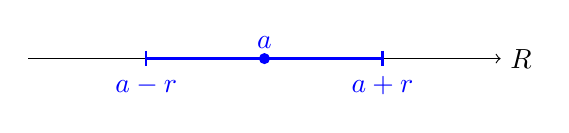
\begin{tikzpicture}
    \draw[->] (-3,0) -- (3,0) node[right] {$\mathbb{R}$};
    \draw[thick, blue] (-1.5,0) -- (1.5,0);
    \draw[blue, thick] (-1.5, 0.1) -- (-1.5, -0.1) node[below] {$a-r$};
    \draw[blue, thick] (1.5, 0.1) -- (1.5, -0.1) node[below] {$a+r$};
    \fill[blue] (0,0) circle (2pt) node[above] {$a$};
\end{tikzpicture}
\end{figure}

\subsubsection*{ii.}
$$ X = \mathbb{R}^n, \quad d_2(x, y) = \sqrt{\sum_{i=1}^n (x_i - y_i)^2} $$

\begin{proof}
\begin{enumerate}
    \item La raíz cuadrada de una suma de cuadrados es no negativa y se anula solo si cada término es
    cero ($x_i = y_i$).
    \item $(x_i - y_i)^2 = (y_i - x_i)^2$, por lo que la suma es igual.
    \item La desigualdad triangular es la desigualdad de Minkowski para sumas:
    $\|x - z\|_2 \le \|x - y\|_2 + \|y - z\|_2$.
\end{enumerate}
\end{proof}

Bola Abierta ($n=2$): Es el interior de un círculo usual.

\subsubsection*{iii.}
$$ X = \mathbb{R}^n, \quad d_1(x, y) = \sum_{i=1}^n |x_i - y_i| $$

\begin{proof}
Las propiedades 1 y 2 se deducen de las del valor absoluto en cada coordenada. Para la triangular,
en cada componente $i$ vale $|x_i - z_i| \le |x_i - y_i| + |y_i - z_i|$; sumando sobre $i$ se obtiene
la desigualdad para la métrica.
\end{proof}

Bola Abierta ($n=2$): $|x_1 - a_1| + |x_2 - a_2| < r$. Es un cuadrado rotado a 45 grados.

\subsubsection*{iv.}
$$ X = \mathbb{R}^n, \quad d_\infty(x, y) = \max_{1 \le i \le n} |x_i - y_i| $$

\begin{proof}
El máximo de valores no negativos es no negativo y se anula solo si todos lo hacen, y la simetría se
hereda del valor absoluto. Para la triangular, sea $k$ el índice donde se alcanza el máximo de
$|x_i - z_i|$; entonces
$$ d_\infty(x, z) = |x_k - z_k| \le |x_k - y_k| + |y_k - z_k| \le d_\infty(x, y) + d_\infty(y, z), $$
pues cada término es menor o igual que su respectivo máximo.
\end{proof}

Bola Abierta ($n=2$): $\max(|x_1 - a_1|, |x_2 - a_2|) < r$. Es un cuadrado con lados paralelos a los
ejes.

\begin{figure}[H]
\centering
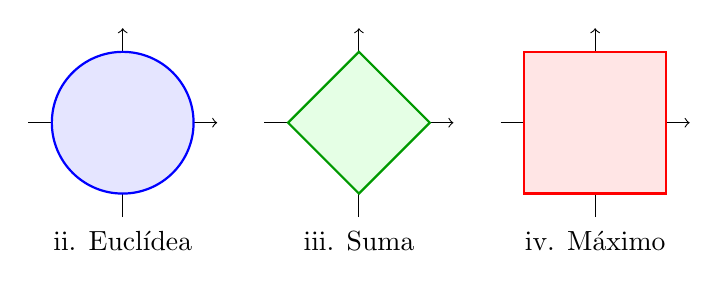
\begin{tikzpicture}[scale=0.6]
    % Euclídea
    \begin{scope}[xshift=-5cm]
        \draw[->] (-2,0) -- (2,0); \draw[->] (0,-2) -- (0,2);
        \draw[thick, blue, fill=blue!10] (0,0) circle (1.5cm);
        \node at (0, -2.5) {ii. Euclídea};
    \end{scope}
    
    % Suma
    \begin{scope}[xshift=0cm]
        \draw[->] (-2,0) -- (2,0); \draw[->] (0,-2) -- (0,2);
        \draw[thick, green!60!black, fill=green!10] (0,1.5) -- (1.5,0) -- (0,-1.5) -- (-1.5,0) --
        cycle;
        \node at (0, -2.5) {iii. Suma};
    \end{scope}

    % Máximo
    \begin{scope}[xshift=5cm]
        \draw[->] (-2,0) -- (2,0); \draw[->] (0,-2) -- (0,2);
        \draw[thick, red, fill=red!10] (-1.5,-1.5) rectangle (1.5,1.5);
        \node at (0, -2.5) {iv. Máximo};
    \end{scope}
\end{tikzpicture}
\end{figure}

\subsubsection*{v.}
$$ X = C([0,1]), \quad d(f, g) = \max_{t \in [0,1]} |f(t) - g(t)| $$

\begin{proof}
Análoga a la métrica del máximo en $\mathbb{R}^n$, tomando el máximo sobre el intervalo continuo
$t \in [0,1]$.
\end{proof}

Bola Abierta: Es una franja o tubo de ancho $2r$ centrado en la función $f$.

\begin{figure}[H]
\centering
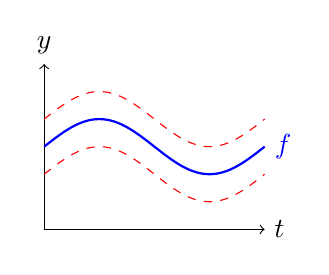
\begin{tikzpicture}[scale=0.7]
    \draw[->] (0,0) -- (4,0) node[right] {$t$};
    \draw[->] (0,0) -- (0,3) node[above] {$y$};
    \draw[thick, blue] (0,1.5) sin (1,2) cos (2,1.5) sin (3,1) cos (4,1.5) node[right] {$f$};
    \draw[dashed, red] (0,2.0) sin (1,2.5) cos (2,2.0) sin (3,1.5) cos (4,2.0);
    \draw[dashed, red] (0,1.0) sin (1,1.5) cos (2,1.0) sin (3,0.5) cos (4,1.0);
\end{tikzpicture}
\end{figure}

\subsubsection*{vi.}
$$ d(x, y) = \begin{cases} 0 & x=y \\ 1 & x \neq y \end{cases} $$

\begin{proof}
Las propiedades 1 y 2 se cumplen por definición. Para la triangular, $d(x, z) \le d(x, y) + d(y, z)$:
si $x \neq z$ entonces $d(x, z) = 1$, y para que la suma de la derecha fuera $0$ debería ser $x = y$
e $y = z$, lo que da $x = z$, contradicción; luego la derecha suma al menos $1$.
\end{proof}

Bola Abierta:
\begin{itemize}
    \item Si $r \le 1$: $B(x, r) = \{x\}$.
    \item Si $r > 1$: $B(x, r) = X$.
\end{itemize}

\subsection*{Ejercicio 2}

Dados $x \in X$ y $r > 0$ fijos, probar que los siguientes conjuntos son abiertos.

\subsubsection*{i. El conjunto $\{y \in X : d(x, y) < r\}$}

Este ejercicio ya fue resuelto.

\subsubsection*{ii. El conjunto $A = \{y \in X : d(x, y) > r\}$}

\begin{proof}
Sea $y_0 \in A$, esto es, $d(x, y_0) = d > r$. Hay que hallar $\delta > 0$ tal que
$B(y_0, \delta) \subset A$. Se define
$$ \delta = d(x, y_0) - r, $$
que es positivo porque $d(x, y_0) > r$. Véase que $B(y_0, \delta) \subset A$: sea
$z \in B(y_0, \delta)$, es decir, $d(y_0, z) < \delta$; hay que ver que $d(x, z) > r$. Por la
desigualdad triangular,
$$ d(x, y_0) \le d(x, z) + d(z, y_0) \implies d(x, z) \ge d(x, y_0) - d(z, y_0). $$
Como $d(z, y_0) < \delta$,
$$ d(x, z) > d(x, y_0) - \delta = d(x, y_0) - (d(x, y_0) - r) = r, $$
de modo que $z \in A$. Luego todo punto de $A$ tiene una bola contenida en $A$, de modo que $A$ es
abierto.
\end{proof}

\subsection*{Ejercicio 3}

Este ejercicio ya fue resuelto.

\subsection*{Ejercicio 4}

Este ejercicio ya fue resuelto.

\subsection*{Ejercicio 5}

Probar las siguientes relaciones entre interior, clausura, uniones e intersecciones.

\subsubsection*{i.}
$$ (A \cap B)^\circ = A^\circ \cap B^\circ $$

\begin{proof}
Se prueba la doble inclusión.

\textit{($\subseteq$).} Sea $x \in (A \cap B)^\circ$. Por definición de interior, existe $r > 0$ con
$$ B(x, r) \subset A \cap B, $$
es decir, todo $y \in B(x, r)$ cumple $y \in A$ e $y \in B$. Luego $B(x, r) \subset A$, de donde
$x \in A^\circ$, y $B(x, r) \subset B$, de donde $x \in B^\circ$; así $x \in A^\circ \cap B^\circ$.

\textit{($\supseteq$).} Sea $x \in A^\circ \cap B^\circ$. Existen $r_1, r_2 > 0$ con
$B(x, r_1) \subset A$ y $B(x, r_2) \subset B$. Con $r = \min\{r_1, r_2\}$, la bola $B(x, r)$ está
contenida en ambas, de modo que $B(x, r) \subset A \cap B$ y $x \in (A \cap B)^\circ$.
\end{proof}

\subsubsection*{ii.}
$$ A^\circ \cup B^\circ \subset (A \cup B)^\circ $$

\begin{proof}
Sea $x \in A^\circ \cup B^\circ$, es decir, $x \in A^\circ$ o $x \in B^\circ$. Si $x \in A^\circ$,
existe $r > 0$ con $B(x, r) \subset A \subset A \cup B$, de modo que $x \in (A \cup B)^\circ$; el caso
$x \in B^\circ$ es análogo. En cualquier caso $x \in (A \cup B)^\circ$.
\end{proof}

La inclusión puede ser estricta. En $\mathbb{R}$ usual, con $A = [0, 1]$ y $B = [1, 2]$ se tiene
$A^\circ = (0, 1)$, $B^\circ = (1, 2)$, de modo que $A^\circ \cup B^\circ = (0, 1) \cup (1, 2)$; en
cambio $A \cup B = [0, 2]$ tiene interior $(0, 2)$. El punto $1$ está en $(A \cup B)^\circ$ pero no
en la unión de los interiores.

\subsubsection*{iii.}
$$ \overline{A \cup B} = \overline{A} \cup \overline{B} $$

\begin{proof}
Se prueba la doble inclusión.

\textit{($\supseteq$).} Sea $x \in \overline{A} \cup \overline{B}$. Si $x \in \overline{A}$, para
todo $r > 0$ se tiene $B(x, r) \cap A \neq \emptyset$, y como $A \subset A \cup B$, también
$B(x, r) \cap (A \cup B) \neq \emptyset$, luego $x \in \overline{A \cup B}$. El caso
$x \in \overline{B}$ es análogo.

\textit{($\subseteq$).} Por contrarrecíproco: supóngase $x \notin \overline{A} \cup \overline{B}$;
hay que ver que $x \notin \overline{A \cup B}$. Existen $r_1, r_2 > 0$ con $B(x, r_1) \cap A =
\emptyset$ y $B(x, r_2) \cap B = \emptyset$. Con $r = \min\{r_1, r_2\}$, la bola $B(x, r)$ está
contenida en ambas, de modo que $B(x, r) \cap A = \emptyset$ y $B(x, r) \cap B = \emptyset$; por tanto
$$ B(x, r) \cap (A \cup B) = (B(x, r) \cap A) \cup (B(x, r) \cap B) = \emptyset, $$
de modo que $x \notin \overline{A \cup B}$.
\end{proof}

\subsubsection*{iv.}
$$ \overline{A \cap B} \subset \overline{A} \cap \overline{B} $$

\begin{proof}
Sea $x \in \overline{A \cap B}$. Para todo $r > 0$, $B(x, r) \cap (A \cap B) \neq \emptyset$; sea
$z$ en esa intersección (depende de $r$), de modo que $z \in B(x, r)$, $z \in A$ y $z \in B$.
Entonces $B(x, r) \cap A \neq \emptyset$ y $B(x, r) \cap B \neq \emptyset$ para todo $r$, luego
$x \in \overline{A}$ y $x \in \overline{B}$, es decir, $x \in \overline{A} \cap \overline{B}$.
\end{proof}

La inclusión puede ser estricta. En $\mathbb{R}$ usual, con $A = (0, 1)$ y $B = (1, 2)$ se tiene
$A \cap B = \emptyset$, de modo que $\overline{A \cap B} = \emptyset$; en cambio $\overline{A} = [0, 1]$
y $\overline{B} = [1, 2]$, con $\overline{A} \cap \overline{B} = \{1\} \neq \emptyset$.

\subsection*{Ejercicios 6}

Este ejercicio ya fue resuelto.

\subsection*{Ejercicios 7}

Este ejercicio ya fue resuelto.

\subsection*{Ejercicios 8}

Este ejercicio ya fue resuelto.

\subsection*{Ejercicio 9}

Probar que si $A \subset B$, entonces el diámetro de $A$ es menor o igual al diámetro de $B$, es
decir, $d(A) \le d(B)$.

\begin{proof}
El diámetro de un conjunto no vacío es $d(A) = \sup \{ d(x, y) : x, y \in A \}$. Considérense los
conjuntos de distancias
$$ S_A = \{ d(x, y) : x, y \in A \}, \qquad S_B = \{ d(u, v) : u, v \in B \}. $$
Sea $r \in S_A$; existen $x_0, y_0 \in A$ con $r = d(x_0, y_0)$. Como $A \subset B$, también
$x_0, y_0 \in B$, de modo que $r = d(x_0, y_0) \in S_B$. Luego $S_A \subseteq S_B$, y como el supremo es
monótono respecto de la inclusión,
$$ d(A) = \sup(S_A) \le \sup(S_B) = d(B). $$
\end{proof}

\subsection*{Ejercicio 10}

Probar que el conjunto de los números irracionales $\mathbb{R} \setminus \mathbb{Q}$ no es una unión
numerable de cerrados.

\begin{proof}
Razónese por el absurdo: supóngase que los irracionales $\mathbb{I} = \mathbb{R} \setminus \mathbb{Q}$
se escriben como unión numerable de cerrados,
$$ \mathbb{I} = \bigcup_{n=1}^{\infty} F_n, $$
con cada $F_n$ cerrado en $\mathbb{R}$. Cada $F_n \subset \mathbb{I}$, y como los irracionales no
contienen ningún intervalo abierto (los racionales son densos), el interior de cada $F_n$ es vacío,
$(F_n)^\circ = \emptyset$.

Por otro lado, $\mathbb{Q}$ es numerable, $\mathbb{Q} = \bigcup_{k=1}^{\infty} \{q_k\}$, y cada
$\{q_k\}$ es cerrado con interior vacío. Entonces
$$ \mathbb{R} = (\mathbb{R} \setminus \mathbb{Q}) \cup \mathbb{Q}
= \left( \bigcup_{n} F_n \right) \cup \left( \bigcup_{k} \{q_k\} \right) $$
queda escrito como unión numerable de cerrados con interior vacío, es decir, $\mathbb{R}$ sería de
primera categoría. Pero $\mathbb{R}$ con la métrica usual es completo, de modo que por el Teorema de
Baire \ref{teo:baire_v2} es de segunda categoría, contradicción. Luego los irracionales no son unión
numerable de cerrados.
\end{proof}

\subsection*{Ejercicio 11}

Dada $f \in C([0,1])$, se definen las integrales iteradas $f_n$. Probar que si para cada
$x \in [0,1]$ existe un $n \in \mathbb{N}$ tal que $f_n(x)=0$, entonces $f=0$.

\begin{proof}
Sea $Z = \{ x \in [0, 1] : f(x) = 0 \}$ el conjunto de ceros de $f$. Como $f$ es continua, $Z$ es
cerrado (se ve en el siguiente capítulo); hay que ver que $Z = [0, 1]$. Sea $U = Z^\circ$ el mayor
abierto donde $f$ se anula; se prueba que $U$ es denso en $[0, 1]$.

Supóngase, por el absurdo, que $U$ no es denso: existe un intervalo abierto no vacío
$(a, b) \subset [0, 1]$ con $(a, b) \cap U = \emptyset$. El intervalo cerrado $K = [a, b]$ es un
subespacio completo (cerrado en un completo). Por hipótesis, para cada $x \in K$ existe $n$ con
$f_n(x) = 0$, de modo que con
$$ F_n = \{ x \in K : f_n(x) = 0 \} $$
se tiene $K = \bigcup_{n=1}^{\infty} F_n$. Como $K$ es completo, por el Teorema de Baire
\ref{teo:baire_v2} algún $F_N$ tiene interior no vacío relativo a $K$: existe $(c, d) \subset (a, b)$
con $f_N \equiv 0$ en $(c, d)$. Derivando $N$ veces (usando $f_k' = f_{k-1}$),
$$ f_N(x) = 0 \implies f_{N-1}(x) = 0 \implies \dots \implies f(x) = 0 \quad \forall x \in (c, d), $$
de modo que $(c, d) \subset Z^\circ = U$. Pero $(c, d) \subset (a, b)$, lo que contradice
$(a, b) \cap U = \emptyset$.

Luego $U$ es denso en $[0, 1]$. Como $f$ es continua y se anula en el conjunto denso $U$, se anula en
todo el espacio: $f(x) = 0$ para todo $x \in [0, 1]$.
\end{proof}

\newpage

\section{Compacidad, continuidad y convergencia}

\subsection{Definiciones Preliminares}

\begin{definicion}{Cubrimiento por abiertos}{cubrimiento}
Una familia $\{U_i\}_{i \in I}$ de abiertos es un cubrimiento abierto de $K \subset X$ si
$K \subseteq \bigcup_i U_i$.
\end{definicion}

\begin{definicion}{Subcubrimiento Finito}{subcubrimiento}
Un cubrimiento $\{U_i\}$ tiene subcubrimiento finito si existen $i_1, \dots, i_n$ con
$K \subseteq U_{i_1} \cup \cdots \cup U_{i_n}$.
\end{definicion}

\subsection{Definición de Conjunto Compacto}

\begin{definicion}{Compacidad}{def_compacto}
$K$ es compacto si todo cubrimiento abierto admite subcubrimiento finito.
\end{definicion}

\subsection{Propiedades en Espacios Métricos}

\begin{proposicion}{Compacto implica Cerrado}{compacto_es_cerrado}
Todo compacto $K$ de un espacio métrico es cerrado.
\end{proposicion}

\begin{proof}
Véase que $K^c$ es abierto. Sea $x \notin K$. Para cada $r > 0$ se define
$$ U_r = \{y \in X : d(x, y) > r\}, $$
abierto. Para cualquier $z \in K$, $d(x,z) > 0$, de modo que $z \in U_{d(x,z)/2}$. Luego
$\{U_r\}_{r > 0}$ es cubrimiento abierto de $K$.

Por compacidad, hay un subcubrimiento finito $U_{r_1}, \dots, U_{r_n}$. Sea
$\bar{r} = \min_j r_j > 0$. Los $U_{r_j}$ son anidados (a menor $r$, más grande $U_r$), de modo que
$\bigcup_j U_{r_j} = U_{\bar r}$, y $K \subseteq U_{\bar r}$. Es decir,
$K \cap \overline{B(x, \bar r)} = \emptyset$. Hay una bola alrededor de $x$ disjunta de $K$.
\end{proof}

\begin{proposicion}{Compacto implica Acotado}{compacto_es_acotado}
Todo compacto $K$ está acotado (vive dentro de una bola).
\end{proposicion}

\begin{proof}
Sea $x_0 \in K$. La familia $\{B(x_0, n)\}_{n \in \mathbb{N}}$ es un cubrimiento abierto de $K$
(porque todo punto está a distancia finita de $x_0$). Por compacidad hay subcubrimiento finito;
tomando $N$ el máximo de los radios, $K \subseteq B(x_0, N)$.
\end{proof}

\subsection{Relación con Conjuntos Cerrados}

\begin{proposicion}{Cerrado dentro de Compacto}{cerrado_en_compacto}
Si $K$ es compacto y $F \subset K$ cerrado, $F$ es compacto.
\end{proposicion}

\begin{proof}
Dado un cubrimiento abierto $\{U_i\}$ de $F$, agregándole el abierto $F^c$ se obtiene un
cubrimiento de $K$. Por compacidad se extrae uno finito $U_{i_1}, \dots, U_{i_n}, F^c$; como
$F \cap F^c = \emptyset$, los $U_{i_j}$ alcanzan para cubrir $F$.
\end{proof}

\obs En $\mathbb{R}^n$ con la métrica usual vale la recíproca: compacto $\iff$ cerrado y
acotado. En general no. Por ejemplo, un conjunto infinito con la métrica discreta es cerrado y
acotado (diámetro 1) pero el cubrimiento por bolas de radio $1/2$ (cada una es un punto) no admite
subcubrimiento finito.


\subsection{Compacidad Secuencial}

\begin{definicion}{Compacidad Secuencial}{secuencial_compacto}
$K$ es secuencialmente compacto si toda sucesión en $K$ admite una subsucesión que converge a un
punto de $K$.
\end{definicion}

\subsection{Conjuntos Totalmente Acotados}

\begin{definicion}{Totalmente Acotado}{totalmente_acotado}
$K$ es totalmente acotado si para todo $\epsilon > 0$ existen $x_1, \dots, x_n \in K$ con
$K \subseteq \bigcup_i B(x_i, \epsilon)$. Esos centros forman una $\epsilon$-red.
\end{definicion}

\subsubsection{Relación entre Acotado y Totalmente Acotado}

\begin{proposicion}{Totalmente Acotado implica Acotado}{tot_acot_implica_acot}
Totalmente acotado $\implies$ acotado.
\end{proposicion}

\begin{proof}
Se toman $\epsilon = 1$ y centros $x_1, \dots, x_n$. Sea $M = \max_i d(x_1, x_i)$.
Para $z \in K$ hay $k$ con $d(z, x_k) < 1$,
de modo que $d(z, x_1) \le d(z, x_k) + d(x_k, x_1) < 1 + M$.
Luego $K \subseteq B(x_1, M+1)$.
\end{proof}

\begin{proposicion}{Secuencialmente Compacto implica Totalmente Acotado}{sec_comp_tot_acot}
Secuencialmente compacto $\implies$ totalmente acotado.
\end{proposicion}

\begin{proof}
Razónese por el absurdo: si no fuera totalmente acotado, existiría $\epsilon > 0$ tal que ninguna
$\epsilon$-red finita cubre $K$.
Se construye $(x_n)$ así: $x_1 \in K$ cualquiera; dados $x_1, \dots, x_n$,
como las bolas $B(x_i, \epsilon)$ no cubren $K$, se toma $x_{n+1}$ fuera.
Por construcción $d(x_n, x_m) \ge \epsilon$ para $n \ne m$,
de modo que ninguna subsucesión de $(x_n)$ puede ser de Cauchy, y entonces ninguna converge.
Contradice la compacidad secuencial.
\end{proof}

\subsection{Lema de Número de Lebesgue}

\begin{proposicion}{Lema de Lebesgue}{lema_lebesgue}
Si $K$ es secuencialmente compacto y $\{U_i\}$ un cubrimiento abierto de $K$, existe $\eta > 0$ (el
número de Lebesgue) tal que toda bola $B(x, \eta)$ con $x \in K$ cabe en algún $U_i$.
\end{proposicion}

\begin{proof}
Razónese por el absurdo: si no existe tal $\eta$, para cada $n$ hay $x_n \in K$ con $B(x_n, 1/n)$ no contenida
en ningún $U_i$. Por compacidad secuencial $(x_n)$ tiene subsucesión $x_{n_k} \to x \in K$. Como
$\{U_i\}$ cubre $K$, hay $U_{i_0}$ con $x \in U_{i_0}$, y existe $r > 0$ con
$B(x, r) \subseteq U_{i_0}$. Eligiendo $k$ grande con $d(x_{n_k}, x) < r/2$ y $1/n_k < r/2$, por la
desigualdad triangular $B(x_{n_k}, 1/n_k) \subseteq B(x, r) \subseteq U_{i_0}$. Contradicción.
\end{proof}

\subsection{Equivalencia de Compacidad}

\begin{teorema}{Teorema de Equivalencia}{equiv_compacidad}
$K$ es compacto si y solo si es secuencialmente compacto.
\end{teorema}

\begin{proof}
Se prueban las dos implicaciones.

\textit{($\Rightarrow$)} Sea $(x_n) \subset K$.
Si el conjunto de valores $S = \{x_n\}$ es finito, algún valor se repite infinitas veces
y se obtiene una subsucesión constante.
Si $S$ es infinito, véase que tiene un punto de acumulación en $K$
(que entonces da la subsucesión por la caracterización \ref{prop:acumulacion_sucesiones}).
Razónese por el absurdo: si no lo tuviera, cada $z \in K$ tendría $r_z > 0$ con
$B(z, r_z) \cap S \subseteq \{z\}$.
La familia $\{B(z, r_z)\}_{z \in K}$ cubre $K$; por compacidad se extrae un
subcubrimiento finito $B(z_1, r_{z_1}), \dots, B(z_m, r_{z_m})$.
Entonces $S$ queda cubierto y tiene a lo sumo $m$ elementos, absurdo.

\textit{($\Leftarrow$)} Sea $\{U_i\}$ un cubrimiento abierto.
Por Lebesgue existe $\eta > 0$ tal que toda bola de radio $\eta$ cabe en algún $U_i$;
por ser totalmente acotado, $K$ se cubre con finitas $B(x_j, \eta)$, $j = 1, \dots, n$.
Se toman $i_j$ con $B(x_j, \eta) \subseteq U_{i_j}$, y $K \subseteq \bigcup_j U_{i_j}$.
\end{proof}

\subsection{Caracterización Métrica de la Compacidad}

\begin{teorema}{Compacidad, Acotación Total y Completitud}{carac_metrica_compacidad}
$K$ es compacto si y solo si es totalmente acotado y completo.
\end{teorema}

\begin{proof}
Se prueban las dos implicaciones.

\textit{($\Rightarrow$)} Ya se vio que secuencialmente compacto $\implies$ totalmente acotado. Para
completitud, una sucesión de Cauchy en $K$ tiene una subsucesión convergente (compacidad
secuencial), y una de Cauchy con una subsucesión convergente converge al mismo límite.

\textit{($\Leftarrow$)} Sea $(x_n) \subset K$; se busca una subsucesión convergente. Argumento de
diagonalización:
\begin{itemize}
    \item \textit{Paso 1.} $K$ se cubre con finitas bolas de radio 1. Alguna de ellas, $B_1$,
    contiene infinitos términos de $(x_n)$. Sea $(x_n^{(1)})$ esa subsucesión.
    \item \textit{Paso $k$.} Ya se tiene $(x_n^{(k-1)})$. Como $K$ se cubre con finitas bolas de
    radio $1/k$, alguna $B_k$ contiene infinitos términos de $(x_n^{(k-1)})$; sea $(x_n^{(k)})$ la
    subsucesión correspondiente.
\end{itemize}
Se define la \emph{diagonal} $y_k = x_k^{(k)}$. Es subsucesión de $(x_n)$ (los índices son
crecientes porque cada $(x_n^{(k)})$ es subsucesión de la anterior).

$(y_k)$ es de Cauchy: para $j, \ell \ge N$, $y_j$ e $y_\ell$ son ambos términos de $(x_n^{(N)})$
(porque las subsucesiones se anidan), y por lo tanto viven en $B_N$, que tiene radio $1/N$. Así
$d(y_j, y_\ell) \le 2/N$. Por completitud, $(y_k)$ converge a un punto de $K$.
\end{proof}

\subsection{Teorema de Heine-Borel}

\begin{teorema}{Heine-Borel}{heine_borel}
$K \subset \mathbb{R}^n$ es compacto si y solo si es cerrado y acotado.
\end{teorema}

\begin{proof}
Se prueban las dos implicaciones.

\textit{($\Rightarrow$)} Ya visto en general.

\textit{($\Leftarrow$)} Si $K$ es acotado, $K \subset [-M, M]^n$ para algún $M$.
Como cerrado en compacto es compacto (\ref{prop:cerrado_en_compacto}), basta ver que
$C = [-M, M]^n$ es compacto.
Es completo (cerrado de $\mathbb{R}^n$, que es completo) y totalmente acotado:
dado $\epsilon > 0$, en cada coordenada $[-M, M]$ existe una $\epsilon/n$-red finita
$\{a_1, \dots, a_p\}$; el producto $\{a_1, \dots, a_p\}^n$ es una $\epsilon$-red para $C$
(cambiando coordenada por coordenada con la triangular,
$d(x, a) \le \sum_i |x_i - a_{k_i}| < \epsilon$).
\end{proof}

\subsection{Continuidad en Espacios Métricos}

\begin{definicion}{Función Continua}{def_continuidad}
$f: X \to Y$ es \textbf{continua} en $a \in X$ si para todo $\epsilon > 0$ existe $\delta > 0$ con
$f(B_X(a, \delta)) \subseteq B_Y(f(a), \epsilon)$. $f$ es continua si lo es en todo punto.
\end{definicion}

\subsection{Equivalencias de la Continuidad}

\begin{teorema}{Caracterizaciones de la Continuidad}{equiv_continuidad}
Para $f: X \to Y$ son equivalentes:
\begin{enumerate}
    \item[i)] $f$ es continua.
    \item[ii)] $f^{-1}(U)$ es abierto en $X$ para todo $U$ abierto en $Y$.
    \item[iii)] $x_n \to x \implies f(x_n) \to f(x)$.
\end{enumerate}
\end{teorema}

\begin{proof}
Se prueba en cadena $(i) \Rightarrow (ii) \Rightarrow (iii) \Rightarrow (i)$.

\textit{(i) $\Rightarrow$ (ii):} Sea $U$ abierto y $a \in f^{-1}(U)$. Como $U$ es abierto, hay
$\epsilon > 0$ con $B(f(a), \epsilon) \subset U$; por continuidad hay $\delta$ con
$f(B(a, \delta)) \subset B(f(a), \epsilon) \subset U$, de modo que $B(a, \delta) \subset f^{-1}(U)$.

\textit{(ii) $\Rightarrow$ (iii):} Si $x_n \to x$ y $\epsilon > 0$, $V = B(f(x), \epsilon)$ es
abierto y $f^{-1}(V)$ es abierto con $x \in f^{-1}(V)$. Hay $r > 0$ con $B(x, r) \subset f^{-1}(V)$;
para $n$ grande, $x_n \in B(x, r)$ y $f(x_n) \in V$.

\textit{(iii) $\Rightarrow$ (i):} Por contrarrecíproco. Si $f$ no es continua en $a$, hay
$\epsilon > 0$ tal que para cada $\delta = 1/n$ existe $x_n$ con $d(x_n, a) < 1/n$ pero
$d(f(x_n), f(a)) \ge \epsilon$. Entonces $x_n \to a$ y $f(x_n) \not\to f(a)$.
\end{proof}

\subsection{Funciones Continuas y Compacidad}

\begin{teorema}{Preservación de la Compacidad}{preservacion_compacidad}
Si $f: X \to Y$ es continua y $K \subset X$ compacto, $f(K)$ es compacto.
\end{teorema}

\begin{proof}
Dado un cubrimiento abierto $\{U_i\}$ de $f(K)$, las preimágenes $V_i = f^{-1}(U_i)$ son abiertas
y cubren $K$. Por compacidad, hay subcubrimiento finito $V_{i_1}, \dots, V_{i_n}$; entonces
$U_{i_1}, \dots, U_{i_n}$ cubren $f(K)$.
\end{proof}

\subsection{Teorema de Weierstrass}

\begin{corolario}{Existencia de Máximo y Mínimo}{weierstrass}
Si $K$ es compacto y $f: K \to \mathbb{R}$ continua, $f$ alcanza máximo y mínimo en $K$.
\end{corolario}

\begin{proof}
$f(K)$ es compacto en $\mathbb{R}$, de modo que es cerrado y acotado (Heine-Borel
\ref{teo:heine_borel}). Cerrado y acotado
implica que el supremo e ínfimo existen y están en $f(K)$ (un cerrado contiene a sus puntos
límite, en particular a sus extremos). Luego hay $x_{\max}, x_{\min} \in K$ con
$f(x_{\max}) = \sup$ y $f(x_{\min}) = \inf$.
\end{proof}

\subsection{Continuidad Uniforme}

La continuidad usual es local (en un punto $a$). La continuidad uniforme es global: pide un control
uniforme en todo el dominio a la vez.

\subsubsection{Motivación: Dependencia del Punto}

$f(x) = 1/x$ en $(0, \infty)$ es continua en todo punto. Dado $a > 0$ y $\epsilon > 0$,
$$ \left|\frac{1}{x} - \frac{1}{a}\right| = \frac{|x-a|}{xa}. $$
Acotando $x > a/2$, queda $\frac{|x-a|}{xa} < \frac{2}{a^2}|x-a|$, de modo que
$\delta \approx a^2 \epsilon / 2$.

El $\delta$ depende de $a$: cuando $a \to 0$, $\delta$ se vuelve arbitrariamente pequeño. No hay un
$\delta$ único que sirva en todo el dominio.

\textit{Consecuencia.} Esta falta de uniformidad rompe la preservación de sucesiones de Cauchy. La
sucesión $x_n = 1/n$ es de Cauchy en $(0, \infty)$ pero $f(x_n) = n$ no lo es.

\subsection{Definición de Continuidad Uniforme}

\begin{definicion}{Continuidad Uniforme}{def_cont_uniforme}
$f: X \to Y$ es \textbf{uniformemente continua} si para todo $\epsilon > 0$ existe $\delta > 0$ tal que para
todo $x, y \in X$,
$$ d_X(x, y) < \delta \implies d_Y(f(x), f(y)) < \epsilon. $$
\end{definicion}

La diferencia está en el orden de los cuantificadores: en continuidad puntual, $\delta$ se elige
después de fijar $x$; en uniforme, $\delta$ se elige antes y sirve para todos los puntos.

\begin{ejemplo}{Funciones Lipschitz}{ej_lipschitz}
$f(x) = mx + b$ es uniformemente continua: $|f(x) - f(y)| = |m||x-y|$, de modo que
$\delta = \epsilon/|m|$ alcanza para todo par de puntos.
\end{ejemplo}

\subsection{Teorema de Heine-Cantor}

\begin{teorema}{Continuidad en Compactos}{heine_cantor}
Si $X$ es compacto y $f: X \to Y$ continua, entonces $f$ es uniformemente continua.
\end{teorema}

\begin{proof}
Sea $\epsilon > 0$. Por continuidad, para cada $x \in X$ hay $\delta_x > 0$ con
$f(B(x, 2\delta_x)) \subseteq B(f(x), \epsilon/2)$ (se toma radio doble para usar la triangular más
tarde). Las $B(x, \delta_x)$ cubren $X$; por compacidad un subcubrimiento finito
$B(x_1, \delta_{x_1}), \dots, B(x_n, \delta_{x_n})$. Se toma $\delta = \min_k \delta_{x_k} > 0$.

Si $d(x, y) < \delta$, hay $k$ con $x \in B(x_k, \delta_{x_k})$, y por la desigualdad triangular
$d(y, x_k) < \delta + \delta_{x_k} \le 2\delta_{x_k}$. Ambos están en $B(x_k, 2\delta_{x_k})$,
de modo que $f(x), f(y) \in B(f(x_k), \epsilon/2)$ y
$$ d(f(x), f(y)) \le d(f(x), f(x_k)) + d(f(x_k), f(y)) < \epsilon. $$
\end{proof}

\subsection{Propiedades básicas}

\begin{proposicion}{Relación con la Continuidad Puntual}{unif_implica_cont}
Uniformemente continua $\implies$ continua en todo punto.
\end{proposicion}

\begin{proof}
Fijando $y = a$ en la definición de continuidad uniforme se recupera la continuidad en $a$.
\end{proof}

\begin{proposicion}{Preservación de Sucesiones de Cauchy}{cauchy_preservation}
Si $f$ es uniformemente continua y $(x_n)$ es de Cauchy, $(f(x_n))$ también es de Cauchy.
\end{proposicion}

\begin{proof}
Dado $\epsilon > 0$, se toman $\delta$ de la continuidad uniforme y $n_0$ tales que
$d(x_n, x_m) < \delta$ para $n, m \ge n_0$. Entonces $d(f(x_n), f(x_m)) < \epsilon$.
\end{proof}

\subsection{Contracciones}

\begin{definicion}{Contracción}{def_contraccion}
$f: X \to X$ es una \textbf{contracción} si existe $\lambda \in [0, 1)$ con
$d(f(x), f(y)) \le \lambda\, d(x, y)$ para todo $x, y$.
\end{definicion}

\subsection{Teorema de Punto Fijo de Banach}

\begin{teorema}{Punto Fijo de Banach}{banach_fixed_point}
Sea $X$ métrico completo y $f: X \to X$ una contracción. Entonces $f$ tiene un único punto
fijo, y para cualquier $x_0 \in X$ la iteración $x_{n+1} = f(x_n)$ converge a él.
\end{teorema}

\begin{proof}
\textit{Existencia.} Fijado $x_0$, sea $x_{n+1} = f(x_n)$. Por inducción,
$$ d(x_{n+1}, x_n) \le \lambda^n d(x_1, x_0). $$
Por la desigualdad triangular y la suma geométrica,
$$ d(x_{n+p}, x_n) \le \sum_{j=0}^{p-1} \lambda^{n+j} d(x_1, x_0) \le \frac{\lambda^n}{1-\lambda}
d(x_1, x_0) \xrightarrow{n \to \infty} 0. $$
Luego $(x_n)$ es de Cauchy. Por completitud converge a algún $x$. Como $f$ es continua
(Lipschitz), $f(x) = \lim f(x_n) = \lim x_{n+1} = x$.

\textit{Unicidad.} Si $f(x) = x$ y $f(y) = y$, $d(x, y) = d(f(x), f(y)) \le \lambda d(x, y)$. Como
$1 - \lambda > 0$, $d(x, y) = 0$.
\end{proof}

\subsection{Otros teoremas clásicos de punto fijo}

\begin{teorema}{Teorema de Brouwer}{teorema_brouwer}
Toda aplicación continua de una bola cerrada de un espacio euclídeo en sí misma admite un punto
fijo.
\end{teorema}

\begin{teorema}{Teorema de Schauder}{teorema_shauder}
Toda aplicación continua de un convexo compacto no vacío K de un espacio de Banach, en K, admite un
punto fijo.
\end{teorema}

\begin{teorema}{Teorema de Kakutani}{teorema_kakutani}
Generaliza a Brouwer para funciones que devuelven conjuntos en lugar de puntos (correspondencias).
Si $F: K \to K$ asigna a cada punto un subconjunto convexo y cerrado, y cumple cierta propiedad de
continuidad (hemicontinuidad superior), entonces existe un punto $x$ tal que $x \in F(x)$.
\end{teorema}

\subsection{Falla de Brouwer en Dimensión Infinita}

Se podría pensar que el teorema de Brouwer vale en cualquier espacio vectorial normado, es decir,
que toda función continua de la bola cerrada unitaria (convexa, cerrada y acotada) en sí misma tiene
punto fijo. Esto es falso en dimensión infinita.

El problema radica en que, en dimensión infinita, la bola cerrada y acotada no es compacta.

\begin{ejemplo}{Contraejemplo en el Espacio de Sucesiones $\ell_2$}{contraejemplo_brouwer}
Considérese el espacio de las sucesiones de cuadrado sumable $\ell_2$, la bola cerrada unitaria
$\overline{B}(0, 1)$ y la función $f: \overline{B}(0, 1) \to \overline{B}(0, 1)$ dada por
$$ f(x_1, x_2, x_3, \dots) = \left( \sqrt{1 - \|x\|^2}, x_1, x_2, \dots \right). $$
\begin{enumerate}
    \item \textit{Está bien definida.} La norma de la imagen es siempre $1$:
    $$ \|f(x)\|^2 = (\sqrt{1 - \|x\|^2})^2 + x_1^2 + x_2^2 + \dots = 1 - \|x\|^2 + \|x\|^2 = 1, $$
    de modo que la imagen cae en la bola (de hecho, en la esfera).
    \item \textit{Es continua.} Sus componentes lo son.
    \item \textit{No tiene punto fijo.} Por el absurdo: supóngase $f(x) = x$. Entonces
    $\|x\| = \|f(x)\| = 1$, e
    igualando la primera coordenada, $x_1 = \sqrt{1 - \|x\|^2} = 0$; igualando la segunda,
    $x_2 = x_1 = 0$, e inductivamente $x_n = 0$ para todo $n$. Luego $x = 0$, cuya norma es $0$, lo
    que contradice $\|x\| = 1$. Por lo tanto no hay punto fijo: $f$ desplaza todos los puntos.
\end{enumerate}
\end{ejemplo}

\subsection{Homeomorfismos}

\begin{definicion}{Homeomorfismo}{def_homeomorfismo}
Una función $f: X \to Y$ es un \textbf{homeomorfismo} si cumple tres condiciones:
\begin{enumerate}
    \item $f$ es biyectiva.
    \item $f$ es continua.
    \item Su inversa $f^{-1}: Y \to X$ también es continua.
\end{enumerate}
\end{definicion}

\begin{proposicion}{Propiedades de los Homeomorfismos}{prop_homeo}
Los homeomorfismos preservan todas las propiedades topológicas. Si $f$ es un homeomorfismo:
\begin{itemize}
    \item $U$ es abierto en $X \iff f(U)$ es abierto en $Y$.
    \item $F$ es cerrado en $X \iff f(F)$ es cerrado en $Y$.
    \item $K$ es compacto en $X \iff f(K)$ es compacto en $Y$.
\end{itemize}
\end{proposicion}

\begin{teorema}{Homeomorfismo en Compactos}{homeo_compacto}
Sea $(X, d_X)$ un espacio métrico compacto y $(Y, d_Y)$ un espacio métrico cualquiera.
Si $f: X \to Y$ es una función continua y biyectiva, entonces $f$ es un homeomorfismo.
(Es decir, $f^{-1}: Y \to X$ es automáticamente continua).
\end{teorema}

\begin{proof}
Como $f$ ya es biyectiva y continua, basta probar que su inversa $f^{-1}$ es continua. Una función
es continua si y solo si la preimagen de todo cerrado es cerrada; aplicado a $f^{-1}$,
$$ f^{-1} \text{ es continua } \iff \forall F \subset X \text{ cerrado}, \ (f^{-1})^{-1}(F)
\text{ es cerrado en } Y. $$
Como la preimagen por la inversa es la imagen directa, $(f^{-1})^{-1}(F) = f(F)$, el objetivo se
reduce a ver que $f$ es cerrada. Sea $F \subset X$ cerrado:
\begin{enumerate}
    \item al ser cerrado en el compacto $X$, $F$ es compacto;
    \item como $f$ es continua, $f(F)$ es compacto en $Y$;
    \item en todo espacio métrico un compacto es cerrado, de modo que $f(F)$ es cerrado en $Y$.
\end{enumerate}
Luego $f$ manda cerrados en cerrados, $f^{-1}$ es continua y $f$ es un homeomorfismo.
\end{proof}

\subsection{Tipos de Convergencia}

Existen dos formas principales en que una sucesión de funciones puede acercarse a una función límite
$f$.

\begin{definicion}{Convergencia Puntual}{conv_puntual}
$(f_n)$ \textbf{converge puntualmente} a $f$ si para cada $x \in K$ fijo la sucesión numérica
$(f_n(x))$ converge a $f(x)$.
$$ \forall x \in K, \quad \lim_{n \to \infty} f_n(x) = f(x) $$
En términos de $\epsilon$: Para todo $\epsilon > 0$ y para todo $x$, existe un $n_0$ (que depende de
$\epsilon$ y de $x$) tal que si $n \ge n_0 \implies |f_n(x) - f(x)| < \epsilon$.
\end{definicion}

La convergencia puntual es débil porque $n_0$ puede crecer sin cota al variar $x$. Para corregir
esto se introduce la convergencia uniforme.

\begin{definicion}{Convergencia Uniforme}{conv_uniforme}
$(f_n)$ \textbf{converge uniformemente} a $f$ si la distancia máxima entre las funciones tiende
a cero.
$$ \lim_{n \to \infty} \left( \sup_{x \in K} |f_n(x) - f(x)| \right) = 0 $$
En términos de $\epsilon$: Para todo $\epsilon > 0$, existe un $n_0$ (que depende solo de
$\epsilon$, no de $x$) tal que para todo $n \ge n_0$ y para todo $x \in K$:
$$ |f_n(x) - f(x)| < \epsilon $$
\end{definicion}

\subsection{El Espacio C(K) y su Completitud}

$C(K)$ es el conjunto de las funciones continuas $f: K \to \mathbb{R}$ con $K$ compacto, equipado
con la norma del supremo $d(f, g) = \max_{x \in K} |f(x) - g(x)|$. Converger en esta métrica es
exactamente converger uniformemente.

\begin{teorema}{Completitud de $C(K)$}{ck_completo}
$(C(K), d_\infty)$ es completo: toda sucesión de Cauchy converge uniformemente a una función
continua.
\end{teorema}

\begin{proof}
Sea $(f_n)$ de Cauchy en $C(K)$.

\textit{Límite puntual.} Para cada $x$, $|f_n(x) - f_m(x)| \le d_\infty(f_n, f_m)$ y $(f_n(x))$ es
de Cauchy en $\mathbb{R}$. Como $\mathbb{R}$ es completo, se define $f(x) = \lim_n f_n(x)$.

\textit{Convergencia uniforme.} Por ser de Cauchy, hay $N$ tal que $|f_n(x) - f_m(x)| < \epsilon$
para todo $x$ y todo $n, m \ge N$. Fijando $n$ y haciendo $m \to \infty$,
$|f_n(x) - f(x)| \le \epsilon$ para todo $x$.

\textit{Continuidad del límite.} Por el argumento del $3\epsilon$: dado $a$ y $\epsilon > 0$, se
elige $n$ grande de modo que $|f(x) - f_n(x)| < \epsilon/3$ uniformemente; luego se usa la
continuidad de $f_n$ para obtener $\delta$ con $|f_n(x) - f_n(a)| < \epsilon/3$ cuando
$d(x, a) < \delta$. Por la desigualdad
triangular,
$$ |f(x) - f(a)| \le |f(x) - f_n(x)| + |f_n(x) - f_n(a)| + |f_n(a) - f(a)| < \epsilon. $$
\end{proof}

\newpage

\subsection{Ejercicios resueltos}

\subsection*{Ejercicio 1}

Probar las implicaciones y dar contraejemplos.

\subsubsection*{i. Compacto $\implies$ Totalmente Acotado}
Esta implicación ya fue demostrada.

Contraejemplo: un conjunto puede ser totalmente acotado pero no compacto. Considérese el intervalo
abierto $(0, 1)$ con la métrica usual.
\begin{itemize}
    \item \textit{Totalmente acotado.} Para cualquier $\epsilon$ se lo cubre con finitos intervalos
    de longitud $\epsilon$.
    \item \textit{No compacto.} El cubrimiento abierto $\{(1/n, 1)\}_{n \in \mathbb{N}}$ no tiene
    subcubrimiento finito (falla por no ser completo).
\end{itemize}

\subsubsection*{ii. Totalmente Acotado $\implies$ Acotado}
Esta implicación ya fue demostrada.

Contraejemplo: un conjunto puede ser acotado pero no totalmente acotado. Considérese un conjunto
infinito $X$ con la métrica discreta.
\begin{itemize}
    \item \textit{Acotado.} Todo el conjunto entra en la bola $B(x, 2)$, pues la distancia máxima es
    $1$.
    \item \textit{No totalmente acotado.} Para $\epsilon = 1/2$, las bolas son puntos individuales
    $\{x\}$, y se necesitarían infinitas para cubrir el conjunto.
\end{itemize}

\subsection*{Ejercicio 2}

Sea $K = \{0\} \cup \{ \frac{1}{n} : n \in \mathbb{N} \} \subset \mathbb{R}$. Probar por definición
que $K$ es compacto.

\begin{proof}
Sea $\{U_i\}_{i \in I}$ un cubrimiento abierto de $K$. Como $0 \in K$, hay $i_0$ con $0 \in U_{i_0}$,
y por ser abierto existe $r > 0$ con $(-r, r) = B(0, r) \subseteq U_{i_0}$. Como $1/n \to 0$, existe
$N$ tal que $1/n < r$ para todo $n \ge N$, de modo que la cola $\{1/n : n \ge N\}$ queda en $U_{i_0}$.
Restan los finitos puntos $1, 1/2, \dots, 1/(N-1)$; para cada $1/k$ se elige un abierto $U_{i_k}$ que
lo contenga. Entonces
$$ \{ U_{i_0}, U_{i_1}, \dots, U_{i_{N-1}} \} $$
es un subcubrimiento finito de $K$. Luego $K$ es compacto.
\end{proof}

\subsection*{Ejercicio 3}

Probar que si un espacio métrico (o subconjunto) es totalmente acotado, entonces es separable.
(Como corolario, todo espacio métrico compacto es separable).

\begin{proof}
Sea $K$ totalmente acotado; se busca $D \subset K$ numerable y denso.

\textit{Construcción de $D$.} Para cada $n \in \mathbb{N}$, con radio $\epsilon_n = 1/n$, la
acotación total da una red finita $F_n = \{x_{n,1}, \dots, x_{n,k_n}\} \subset K$ con
$$ K \subseteq \bigcup_{j=1}^{k_n} B\!\left(x_{n,j}, \tfrac{1}{n}\right). $$
Se define $D = \bigcup_{n=1}^{\infty} F_n$.

\textit{Numerabilidad.} $D$ es unión numerable de conjuntos finitos, luego es numerable.

\textit{Densidad.} $D$ es denso si y solo si corta a todo abierto no vacío de $K$. Sea $U$ abierto no
vacío y $x \in U$, con $B(x, r) \subseteq U$. Por la Propiedad Arquimediana \ref{prop:arquimediana}
existe $N$ con $1/N < r$.
La red $F_N$ cubre $K$ con bolas de radio $1/N$, de modo que hay $z \in F_N$ con $d(x, z) < 1/N < r$, de
donde $z \in B(x, r) \subseteq U$. Como $z \in D \cap U$, se tiene $D \cap U \neq \emptyset$. Luego
$D$ es denso en $K$.
\end{proof}

\subsection*{Ejercicio 4}

Dada una familia de cerrados $(F_{\alpha})$ tales que uno de ellos, $F_{\alpha'}$, es compacto;
probar que $K = \bigcap_{\alpha} F_{\alpha}$ es compacto. ¿Puede ser vacía?

\begin{proof}
La intersección arbitraria de cerrados es cerrada, de modo que $K = \bigcap_\alpha F_\alpha$ es cerrado.
Además $K \subseteq F_{\alpha'}$, de modo que $K$ es un cerrado contenido en el compacto
$F_{\alpha'}$; por la Proposición \ref{prop:cerrado_en_compacto}, $K$ es compacto.
\end{proof}

La intersección puede ser vacía, y el conjunto vacío es compacto. Por ejemplo, en $\mathbb{R}$, con
$F_1 = [0, 1]$ (compacto) y $F_2 = [2, 3]$ (cerrado), se tiene $F_1 \cap F_2 = \emptyset$.

\subsection*{Ejercicio 5}

Probar que $X$ es compacto $\iff$ para toda sucesión $(F_n)$ decreciente de cerrados no vacíos,
$\bigcap_{n=1}^{\infty} F_n \neq \emptyset$.

\begin{proof}
\textit{($\Rightarrow$).} Razónese por el absurdo: supóngase una sucesión $(F_n)$ de cerrados no
vacíos y decrecientes con $\bigcap_{n=1}^{\infty} F_n = \emptyset$. Con $U_n = F_n^c$ (abiertos), por
De Morgan
$$ \bigcup_{n=1}^{\infty} U_n = \left( \bigcap_{n=1}^{\infty} F_n \right)^c = X, $$
de modo que $\{U_n\}$ es un cubrimiento abierto de $X$. Por compacidad hay un subcubrimiento finito
$U_{n_1}, \dots, U_{n_k}$; como $(F_n)$ decrece, $(U_n)$ crece, y con $N = \max\{n_1, \dots, n_k\}$ se
tiene $\bigcup_j U_{n_j} = U_N = X$. Tomando complementos, $F_N = \emptyset$, lo que contradice que
los $F_n$ sean no vacíos.

\textit{($\Leftarrow$).} Por contrarrecíproco: supóngase que $X$ no es compacto. En un espacio
métrico esto da un cubrimiento numerable $\{U_n\}$ sin subcubrimiento finito. Con
$A_n = U_1 \cup \dots \cup U_n$ se define $F_n = X \setminus A_n$. Cada $F_n$ es cerrado (complemento
de unión finita de abiertos), la sucesión decrece ($A_n$ crece, de modo que $F_{n+1} \subset F_n$) y es
no vacía (si algún $A_n = X$, los $U_1, \dots, U_n$ serían un subcubrimiento finito). Sin embargo,
$$ \bigcap_{n=1}^{\infty} F_n = X \setminus \bigcup_{n=1}^{\infty} A_n = X \setminus
\bigcup_{n=1}^{\infty} U_n = X \setminus X = \emptyset. $$
Así se construye una sucesión decreciente de cerrados no vacíos con intersección vacía.
\end{proof}

\subsection*{Ejercicio 6}

Se define la distancia entre dos conjuntos como $d(A, B) = \inf \{ d(x, y) : x \in A, y \in B \}$.

\subsubsection*{i.}
\begin{proposicion}{Distancia Positiva}{dist_compact_closed}
Si $A$ es compacto y $B$ cerrado tales que $A \cap B = \emptyset$, entonces $d(A, B) > 0$.
\end{proposicion}

\begin{proof}
Razónese por el absurdo: supóngase $d(A, B) = 0$. Por definición de ínfimo, para cada $n$ existen
$x_n \in A$ e $y_n \in B$ con $d(x_n, y_n) < 1/n$, de modo que $d(x_n, y_n) \to 0$. Como $A$ es compacto,
es secuencialmente compacto (\ref{teo:equiv_compacidad}), y $(x_n)$ tiene una subsucesión
$x_{n_k} \to a \in A$. Por la
desigualdad triangular,
$$ d(y_{n_k}, a) \le d(y_{n_k}, x_{n_k}) + d(x_{n_k}, a), $$
donde $d(y_{n_k}, x_{n_k}) < 1/n_k \to 0$ y $d(x_{n_k}, a) \to 0$, de modo que $y_{n_k} \to a$. Como
$B$ es cerrado, $a \in B$. Entonces $a \in A \cap B$, lo que contradice $A \cap B = \emptyset$. Luego
$d(A, B) > 0$.
\end{proof}

\subsubsection*{ii.}
Si $A$ y $B$ son solo cerrados disjuntos, puede ocurrir que $d(A, B) = 0$. Como contraejemplo en
$\mathbb{R}^2$, considérense la hipérbola y el eje $x$:
$$ A = \{ (x, y) : xy = 1 \}, \qquad B = \{ (x, y) : y = 0 \}. $$
\begin{itemize}
    \item \textit{Cerrados.} Ambos son preimágenes de cerrados por funciones continuas.
    \item \textit{Disjuntos.} En $A$ la coordenada $y$ nunca es $0$ (pues $xy = 1$); en $B$ siempre
    es $0$.
    \item \textit{Distancia cero.} Con $a_n = (n, 1/n) \in A$ y $b_n = (n, 0) \in B$,
    $$ d(a_n, b_n) = \sqrt{(n-n)^2 + (1/n)^2} = \frac{1}{n} \to 0, $$
    de modo que el ínfimo de las distancias es $0$.
\end{itemize}
Sin compacidad, los conjuntos pueden acercarse asintóticamente sin tocarse.

\subsection*{Ejercicio 7}

Dados subconjuntos compactos $A$ y $B$ de $\mathbb{R}^n$, probar que es compacto el conjunto
$A - B = \{a - b : a \in A, b \in B\}$.

\begin{proof}
Hay que ver que toda sucesión en $A - B$ tiene una subsucesión convergente a un punto de $A - B$.
Sea $(z_n) \subset A - B$, con $z_n = a_n - b_n$, $a_n \in A$, $b_n \in B$. Como $A$ es compacto, hay
una subsucesión $a_{n_k} \to a \in A$. Como $B$ es compacto, $(b_{n_k})$ tiene a su vez una
subsucesión $b_{n_{k_j}} \to b \in B$. Por el álgebra de límites en $\mathbb{R}^n$
(\ref{teo:algebra_limites}),
$$ z_{n_{k_j}} = a_{n_{k_j}} - b_{n_{k_j}} \to a - b, $$
y $a - b \in A - B$. Luego $A - B$ es secuencialmente compacto (\ref{teo:equiv_compacidad}), es decir, compacto.
\end{proof}

\subsection*{Ejercicio 8}

En el conjunto $c_0$ de sucesiones de números reales que tienden a 0, se define la distancia
$d(x, y) = \sup_n |x_n - y_n|$.
Probar que la bola cerrada unitaria $\overline{B}(0, 1)$ no es secuencialmente compacta.

\begin{proof}
Un conjunto es secuencialmente compacto si toda sucesión en él admite una subsucesión convergente.
Se construye una sucesión en $\overline{B}(0, 1)$ sin subsucesiones convergentes.

\textit{Construcción.} Sea $(e^{(n)})$ la sucesión de vectores canónicos, con $e^{(n)}$ la sucesión
que vale $1$ en la posición $n$ y $0$ en el resto.

\textit{Pertenencia.} Cada $e^{(n)}$ tiende a $0$ (es eventualmente nula), de modo que $e^{(n)} \in c_0$,
y $\|e^{(n)}\|_\infty = \sup_k |e^{(n)}_k| = 1$, de modo que $e^{(n)} \in \overline{B}(0, 1)$.

\textit{Distancia entre términos.} Para $n \neq m$, la diferencia $e^{(n)} - e^{(m)}$ vale $1$ en la
posición $n$, $-1$ en la $m$ y $0$ en el resto, de modo que
$$ d(e^{(n)}, e^{(m)}) = \sup_k |e^{(n)}_k - e^{(m)}_k| = 1. $$

\textit{Conclusión.} Por el absurdo: si $(e^{(n_k)})$ convergiera, sería de Cauchy, y sus términos estarían a
distancia $< \epsilon$ entre sí; pero la distancia entre dos términos distintos es siempre $1$. Luego
ninguna subsucesión converge, y $\overline{B}(0, 1)$ no es secuencialmente compacta.
\end{proof}

\subsection*{Ejercicio 9}

\subsubsection*{i.}
Probar que $f: \mathbb{R} \to \mathbb{R}$ tal que $f(x) = x^2$ es continua, pero existe un abierto
$G$ tal que $f(G)$ no es abierto.

\begin{proof}
$f(x) = x^2$ es continua en $\mathbb{R}$. Considérese el abierto $G = (-1, 1)$; su imagen directa es
$$ f(G) = \{ x^2 : -1 < x < 1 \} = [0, 1). $$
El punto $y = 0 \in f(G)$ no es interior: para todo $\epsilon > 0$, la bola
$B(0, \epsilon) = (-\epsilon, \epsilon)$ contiene números negativos, que no están en $[0, 1)$, de modo
que $(-\epsilon, \epsilon) \not\subset [0, 1)$. Luego $f(G)$ no es abierto.
\end{proof}

\subsubsection*{ii.}
Probar que $g: \mathbb{R} \to \mathbb{R}$ tal que $g(x) = \frac{x^2}{1+x^2}$ es continua, pero
existe un cerrado $F$ tal que $g(F)$ no es cerrado.

\begin{proof}
$g$ es continua por ser cociente de polinomios con denominador no nulo ($1 + x^2 \ge 1$). Considérese
el cerrado $F = [0, +\infty)$. En $x = 0$ vale $g(0) = 0$; para $x > 0$ es estrictamente creciente, y
$$ \lim_{x \to +\infty} \frac{x^2}{1+x^2} = 1, $$
de modo que $g(F) = [0, 1)$. La sucesión $y_n = g(n) = \frac{n^2}{1+n^2} \in g(F)$ cumple $y_n \to 1$, de
modo que $1$ es punto de acumulación de $[0, 1)$ pero $1 \notin [0, 1)$. Como le falta un punto
límite, $g(F)$ no es cerrado.
\end{proof}

\subsection*{Ejercicio 10}

Dadas $f, g: X \to Y$ funciones continuas.

\subsubsection*{i.}
Probar que $A = \{x \in X : f(x) \neq g(x)\}$ es abierto.

\begin{proof}
Sea $a \in A$, esto es, $f(a) \neq g(a)$, con $d(f(a), g(a)) = \epsilon > 0$. Con $r = \epsilon/2$,
las bolas $B(f(a), r)$ y $B(g(a), r)$ son disjuntas. Por continuidad, existen
$\delta_1, \delta_2 > 0$ con $f(B(a, \delta_1)) \subset B(f(a), r)$ y
$g(B(a, \delta_2)) \subset B(g(a), r)$. Con $\delta = \min\{\delta_1, \delta_2\}$, para
$x \in B(a, \delta)$ se tiene $f(x) \in B(f(a), r)$ y $g(x) \in B(g(a), r)$; como esas bolas son
disjuntas, $f(x) \neq g(x)$ y $x \in A$. Luego $B(a, \delta) \subset A$, y $A$ es abierto.
\end{proof}

\subsubsection*{ii.}
Deducir que $E = \{x \in X : f(x) = g(x)\}$ es cerrado.

\begin{proof}
El conjunto $E$ es el complemento de $A$: $E = A^c$. Como $A$ es abierto (inciso anterior), su
complemento $E$ es cerrado.
\end{proof}

\subsubsection*{ii. (Alternativo)}

Otra prueba de que $E = \{x \in X : f(x) = g(x)\}$ es cerrado.

\begin{proof}
Se define la función auxiliar $h: X \to \mathbb{R}$, $h(x) = f(x) - g(x)$, que es continua por ser
resta de continuas. Un punto $x$ está en $E$ si y solo si $f(x) = g(x)$, es decir, $h(x) = 0$, de modo
que $E = h^{-1}(\{0\})$. Como $\{0\}$ es cerrado en $\mathbb{R}$ y $h$ es continua, $E$ es cerrado.
\end{proof}

\subsubsection*{iii.}
Probar que si $D$ es denso en $X$ y $f(x) = g(x)$ para todo $x \in D$, entonces $f = g$ en todo $X$.

\begin{proof}
Considérese $E = \{x \in X : f(x) = g(x)\}$. Por hipótesis $D \subseteq E$, y tomando clausura,
$\overline{D} \subseteq \overline{E}$. Como $D$ es denso, $\overline{D} = X$, y como $E$ es cerrado
(inciso ii), $\overline{E} = E$. Luego $X \subseteq E$, es decir, $f(x) = g(x)$ para todo $x \in X$.
\end{proof}

\subsubsection*{iii. (Altermativo)}
Probar que si $D$ es denso en $X$ y $f(x) = g(x)$ para todo $x \in D$, entonces $f = g$ en todo $X$.

\begin{proof}
Sea $x \in X$. Como $D$ es denso, $x \in \overline{D}$, de modo que existe $(d_n) \subset D$ con
$d_n \to x$. Por hipótesis $f(d_n) = g(d_n)$ para todo $n$, y como $f$ y $g$ son continuas,
$f(d_n) \to f(x)$ y $g(d_n) \to g(x)$. Como las sucesiones $(f(d_n))$ y $(g(d_n))$ coinciden término
a término, sus límites son iguales: $f(x) = g(x)$. Como $x$ era arbitrario, $f = g$ en $X$.
\end{proof}

\subsection*{Ejercicio 11}

Dada $f: \mathbb{R} \to \mathbb{R}$ continua tal que existen $a, b \in \mathbb{R}$ con $f(a) < 0$ y
$f(b) > 0$. Probar que existe un $c \in \mathbb{R}$ tal que $f(c) = 0$.

\begin{proof}
Sin pérdida de generalidad, $a < b$. Se define
$$ A = \{ x \in [a, b] : f(x) \le 0 \}. $$
\textit{Existencia del supremo.} Como $f(a) < 0$, $a \in A$, de modo que $A \neq \emptyset$; y
$A \subseteq [a, b]$, de modo que $b$ es cota superior. Por el Axioma de Completitud
(\ref{teo:axioma_completitud}) existe $c = \sup(A)$, con $a \le c \le b$.

\textit{$f(c) = 0$.} Se descartan los otros dos casos por continuidad.

\textit{Caso $f(c) < 0$.} Por continuidad, hay $\delta > 0$ con $f(x) < 0$ en
$(c - \delta, c + \delta)$. Como $f(b) > 0$, es $c < b$, y se puede elegir $x_0$ con
$c < x_0 < c + \delta$; entonces $f(x_0) < 0$, de modo que $x_0 \in A$ con $x_0 > c$, lo que contradice
que $c$ sea cota superior.

\textit{Caso $f(c) > 0$.} Por continuidad, hay $\delta > 0$ con $f(x) > 0$ en
$(c - \delta, c + \delta)$, de modo que ningún punto de $(c - \delta, c]$ está en $A$ y todo $x \in A$
cumple $x \le c - \delta$; entonces $c - \delta < c$ sería cota superior, contra que $c$ sea la
menor.

Luego $f(c) = 0$.
\end{proof}

\subsection*{Ejercicio 12}

Probar que acotado, completo y ser de Cauchy no son propiedades homeomórficas (es decir, no se
preservan necesariamente por homeomorfismos).

Por contraejemplos. Considérense dos espacios métricos clásicos con la métrica usual:
\begin{itemize}
    \item $X = (0, 1)$.
    \item $Y = \mathbb{R}$.
\end{itemize}
Existe un homeomorfismo entre ellos, por ejemplo la tangente escalada:
$$ f: (0, 1) \to \mathbb{R}, \quad f(x) = \tan\left( \pi \left( x - \frac{1}{2} \right) \right) $$
Esta función es biyectiva, continua y su inversa es continua. Sin embargo, las propiedades métricas
no se conservan.

\subsubsection*{i}
\begin{itemize}
    \item El espacio $X = (0, 1)$ es acotado (su diámetro es 1).
    \item Su imagen homeomorfa $Y = \mathbb{R}$ es no acotada.
\end{itemize}
Luego, la acotación no es un invariante topológico.

\subsubsection*{ii.}
\begin{itemize}
    \item El espacio $Y = \mathbb{R}$ es completo (toda sucesión de Cauchy converge).
    \item El espacio $X = (0, 1)$ no es completo.
    \textit{Justificación:} La sucesión $x_n = \frac{1}{n+1}$ está contenida en $(0, 1)$. Es una
    sucesión de Cauchy (porque en $\mathbb{R}$ converge a 0, de modo que los términos se juntan). Sin
    embargo, su límite (0) no pertenece al espacio $(0, 1)$. Por lo tanto, dentro de $X$, la
    sucesión no converge.
\end{itemize}
Como $X \cong Y$ pero uno es completo y el otro no, la completitud no es un invariante topológico.

\subsubsection*{iii.}
Un homeomorfismo puede transformar una sucesión de Cauchy en una que no lo es. Considérese el
homeomorfismo $g: (0, 1) \to (1, +\infty)$ dado por $g(x) = \frac{1}{x}$.

\begin{itemize}
    \item La sucesión $x_n = \frac{1}{n}$ (para $n \ge 2$) está en $(0, 1)$ y es de Cauchy, ya que
    $\left| \frac{1}{n} - \frac{1}{m} \right| \to 0$.
    \item Aplicando $g$, $y_n = g(x_n) = n$.
    \item La sucesión imagen $(2, 3, 4, \dots)$ no es de Cauchy, pues la distancia entre términos
    consecutivos es siempre $1$.
\end{itemize}
Luego, ser una sucesión de Cauchy es una propiedad que depende de la métrica específica y no se
preserva bajo homeomorfismos.

\subsection*{Ejercicio 13}

Este ejercicio ya fue resuelto.

\subsection*{Ejercicio 14}

Probar la continuidad uniforme en los siguientes casos.

\subsubsection*{i.}
$f: \mathbb{R} \to \mathbb{R}$ tal que $f(x) = 2x$.

\begin{proof}
Es Lipschitziana: $|f(x) - f(y)| = 2|x - y|$. Dado $\epsilon > 0$, con $\delta = \epsilon/2$, si
$|x - y| < \delta$ entonces $|f(x) - f(y)| = 2|x - y| < \epsilon$. Luego $f$ es uniformemente
continua.
\end{proof}

\subsubsection*{ii.}
$f: [0, \infty) \to \mathbb{R}$ tal que $f(x) = \sqrt{x}$.

\begin{proof}
% TODO completar la demostración de la continuidad uniforme de $\sqrt{x}$ en $[0,\infty)$.
\end{proof}

\subsubsection*{iii.}
$f: [0, 1] \to \mathbb{R}$ tal que $f(x) = x^2$.

\begin{proof}
$f$ es continua (polinómica) y el dominio $[0, 1]$ es cerrado y acotado, luego compacto en
$\mathbb{R}$. Por el Teorema de Heine-Cantor \ref{teo:heine_cantor}, $f$ es uniformemente continua.
\end{proof}

\subsubsection*{Contraejemplo:}
Probar que $f: \mathbb{R} \to \mathbb{R}$ tal que $f(x) = x^2$ no es uniformemente continua.

\begin{proof}
Por la caracterización con sucesiones: si $f$ fuera uniformemente continua, enviaría sucesiones con
$|x_n - y_n| \to 0$ a sucesiones con $|f(x_n) - f(y_n)| \to 0$. Con $x_n = n$ e $y_n = n + 1/n$,
$$ |x_n - y_n| = \frac{1}{n} \to 0, $$
pero
$$ |f(x_n) - f(y_n)| = \left| n^2 - \left(n + \tfrac{1}{n}\right)^2 \right|
= \left| -2 - \tfrac{1}{n^2} \right| = 2 + \frac{1}{n^2} \to 2 \neq 0. $$
Como la distancia de las imágenes no tiende a $0$, $f$ no es uniformemente continua.
\end{proof}

\subsection*{Ejercicio 15}

Probar que si $f: \mathbb{R} \to \mathbb{R}$ es continua y $\lim_{|x| \to \infty} f(x) = 0$,
entonces $f$ es uniformemente continua.

\begin{proof}
Dado $\epsilon > 0$, hay que hallar un $\delta$ válido en todo $\mathbb{R}$.

\textit{Colas.} Como $\lim_{|x| \to \infty} f(x) = 0$, existe $M > 0$ tal que $|f(x)| < \epsilon/2$
para $|x| > M$.

\textit{Centro.} El intervalo $K = [-M-1, M+1]$ es compacto, de modo que por el Teorema de Heine-Cantor
\ref{teo:heine_cantor} $f$ es uniformemente continua en $K$: existe $\delta_K > 0$ tal que
$|x - y| < \delta_K \implies |f(x) - f(y)| < \epsilon$ para $x, y \in K$.

\textit{Elección de $\delta$.} Se toma $\delta = \min(1, \delta_K)$, y sean $x, y \in \mathbb{R}$ con
$|x - y| < \delta$.
\begin{itemize}
    \item Si $|x| > M$ e $|y| > M$, entonces $|f(x) - f(y)| \le |f(x)| + |f(y)| < \epsilon$.
    \item Si, por ejemplo, $x \in [-M, M]$, como $|x - y| < \delta \le 1$ se tiene
    $|y| \le |x| + 1 \le M + 1$, de modo que $x, y \in K$ y, por la continuidad uniforme en $K$,
    $|f(x) - f(y)| < \epsilon$.
\end{itemize}
En todos los casos $|f(x) - f(y)| < \epsilon$, luego $f$ es uniformemente continua en $\mathbb{R}$.
\end{proof}

\newpage

\section{Clasificación de Espacios y Convexidad}

\begin{definicion}{Espacio de Hilbert}{}
Un \textbf{Hilbert} es un espacio vectorial $H$ con producto interno $\langle\cdot, \cdot\rangle$, completo
respecto a la métrica inducida por $\|x\| = \sqrt{\langle x, x \rangle}$.
\end{definicion}

\begin{definicion}{Espacio de Banach}{}
Un \textbf{Banach} es un espacio normado $(X, \|\cdot\|)$ completo respecto a $d(x,y) = \|x-y\|$.
\end{definicion}

Todo Hilbert es Banach, pero no al revés. Los siguientes son ejemplos clásicos de Banach que no
son Hilbert.

\begin{ejemplo}{El espacio $\ell^1$}{}
$\ell^1 = \{x = (x_n) : \sum |x_n| < \infty\}$, con norma $\|x\|_1 = \sum |x_n|$.
\end{ejemplo}

\begin{ejemplo}{El espacio $\ell^\infty$}{}
$\ell^\infty = \{x = (x_n) : \sup_n |x_n| < \infty\}$, con norma $\|x\|_\infty = \sup_n |x_n|$.
\end{ejemplo}

\begin{definicion}{Espacio de Fréchet}{}
Espacio vectorial topológico localmente convexo, completo, cuya topología está inducida por
una métrica invariante por traslaciones (típicamente por una familia numerable de seminormas).
\end{definicion}

\begin{definicion}{Espacio Localmente Convexo}{}
Espacio topológico cuya topología está generada por una familia de seminormas; o,
equivalentemente, donde el origen tiene una base de entornos convexos.
\end{definicion}

\subsection{Diferencia entre Hilbert y Banach: Ley del Paralelogramo}

\begin{teorema}{Ley del Paralelogramo}{paralelogramo}
La norma de $(X, \|\cdot\|)$ proviene de un producto interno si y solo si para todo $x, y \in X$
vale
$$ \|x + y\|^2 + \|x - y\|^2 = 2(\|x\|^2 + \|y\|^2). $$
\end{teorema}

\obs $\ell^1$ y $\ell^\infty$ no cumplen la ley del paralelogramo: con los canónicos $e_1, e_2$ ya
falla. Por eso son Banach pero no Hilbert.

\obs (Identidad de polarización). Cuando vale el paralelogramo, el producto interno se recupera a
partir de la norma:
$$ \langle x, y \rangle = \tfrac{1}{4}\left(\|x + y\|^2 - \|x - y\|^2\right). $$

\subsection{Convexidad y Continuidad}

\begin{definicion}{Conjunto Convexo}{}
$C$ es \textbf{convexo} si $tx + (1-t)y \in C$ para todo $x, y \in C$ y $t \in [0,1]$.
\end{definicion}

\begin{proposicion}{Convexidad de la Bola Cerrada}{}
$\overline{B}(0,1) = \{x : \|x\| \le 1\}$ es convexa en todo espacio normado.
\end{proposicion}

\begin{proof}
Para $x, y$ con $\|x\|, \|y\| \le 1$ y $t \in [0,1]$, por la desigualdad triangular y la homogeneidad
$\|tx + (1-t)y\| \le t\|x\| + (1-t)\|y\| \le 1$.
\end{proof}

\subsubsection{Relación con la continuidad de la suma}
La prueba anterior depende de la triangular $\|x+y\| \le \|x\| + \|y\|$, que es la misma propiedad
que garantiza la continuidad de la suma $+: X \times X \to X$. Geométricamente, la convexidad de
la bola dice que combinaciones convexas (promedios) no se escapan del entorno. En espacios
localmente convexos se pide explícitamente que el origen tenga base de entornos convexos para que
la topología juegue bien con la estructura lineal.

\subsection{Relación entre espacios de sucesiones y compacidad}

\begin{proposicion}{Inclusión de $\ell^1$ en $\ell^\infty$}{}
$\ell^1 \subset \ell^\infty$ con $\|x\|_\infty \le \|x\|_1$.
\end{proposicion}

\begin{proof}
Para cada $k$, $|x_k| \le \sum_n |x_n| = \|x\|_1$; tomando sup en $k$, $\|x\|_\infty \le \|x\|_1$.
\end{proof}

\begin{ejemplo}{}{}
La bola unitaria $\overline{B}_{\ell^1}(0,1)$ no es secuencialmente compacta. Los canónicos
$e^{(n)}$ (un 1 en la posición $n$, cero en el resto) cumplen $\|e^{(n)}\|_1 = 1$. Pero para
$n \ne m$,
$$ \|e^{(n)} - e^{(m)}\|_1 = 2, $$
de modo que ninguna subsucesión es de Cauchy y, como $\ell^1$ es completo, ninguna converge.
\end{ejemplo}

\subsection{\texorpdfstring{Espacios $L^p$ y $\ell^p$}{Espacios Lp y lp}}

Los $\ell^1$ y $\ell^\infty$ vistos antes son los dos extremos de una familia mucho más amplia.

\begin{definicion}{Espacio $L^p$}{Lp}
Sea $(X, \mathcal{A}, \mu)$ un espacio de medida y $1 \le p < \infty$. El espacio $L^p(\mu)$ (o
$L^p$ a secas) es el conjunto de las funciones medibles $f: X \to \mathbb{R}$ con
$$ \int_X |f|^p \, d\mu < \infty. $$
A cada una se le asigna
$$ \|f\|_p = \left( \int_X |f|^p \, d\mu \right)^{1/p}. $$
\end{definicion}

\obs
$\|\cdot\|_p$ no es propiamente una norma sino una seminorma: cumple $\|af\|_p = |a|\,\|f\|_p$ y la
desigualdad triangular (Minkowski, más abajo), pero $\|f\|_p = 0$ solo dice que $f = 0$ en casi todo punto, no
en todos. Para que sea norma se cocientea por la relación ``iguales en casi todo punto''.

\begin{ejemplo}{El espacio $\ell^p$ como caso particular}{ellp}
Si $X = \mathbb{N}$ con la medida de conteo ($\mu(\{n\}) = 1$ para todo $n$), las funciones son
sucesiones $a = (a_n)$ y la integral se vuelve una suma. Queda
$$ \ell^p = \left\{ a = (a_n)_{n \in \mathbb{N}} : \sum_{n=1}^{\infty} |a_n|^p < \infty \right\},
\qquad \|a\|_p = \left( \sum_{n=1}^{\infty} |a_n|^p \right)^{1/p}. $$
\end{ejemplo}

\begin{proposicion}{Inclusión entre espacios $\ell^p$}{inclusion_lp}
Si $1 \le p_1 < p_2 \le \infty$, entonces $\ell^{p_1} \subseteq \ell^{p_2}$ y
$\|a\|_{p_2} \le \|a\|_{p_1}$ para todo $a \in \ell^{p_1}$.
\end{proposicion}

\begin{proof}
Si $a \in \ell^{p_1}$ con $\|a\|_{p_1} = 0$, entonces $a = 0$ y no hay nada que probar. Por
homogeneidad puede suponerse $\|a\|_{p_1} = 1$. Entonces $|a_n|^{p_1} \le 1$ para todo $n$, en
particular $|a_n| \le 1$. Como $p_2 > p_1$ y $|a_n| \le 1$, vale $|a_n|^{p_2} \le |a_n|^{p_1}$.
Sumando,
$$ \|a\|_{p_2}^{p_2} = \sum |a_n|^{p_2} \le \sum |a_n|^{p_1} = \|a\|_{p_1}^{p_1} = 1, $$
de modo que $\|a\|_{p_2} \le 1 = \|a\|_{p_1}$. Para $p_2 = \infty$,
$\|a\|_\infty = \sup_n |a_n| \le 1$.
\end{proof}

\begin{proposicion}{Inclusión en medida finita}{inclusion_lp_finita}
Si $\mu(X) < \infty$ y $1 \le p_1 < p_2 < \infty$, entonces $L^{p_2}(\mu) \subseteq L^{p_1}(\mu)$.
\end{proposicion}

\begin{proof}
Sea $f \in L^{p_2}$. Se parte $X$ según donde $|f|$ es grande o pequeño: $A = \{|f| \le 1\}$,
$A^c = \{|f| > 1\}$. En $A$, $|f|^{p_1} \le 1$. En $A^c$, $|f|^{p_1} < |f|^{p_2}$ (porque $|f| > 1$
y $p_1 < p_2$). Así,
$$ \int_X |f|^{p_1} d\mu = \int_A |f|^{p_1} d\mu + \int_{A^c} |f|^{p_1} d\mu \le \mu(A) + \int_{A^c}
|f|^{p_2} d\mu \le \mu(X) + \|f\|_{p_2}^{p_2} < \infty. $$
\end{proof}

\obs En medida infinita la inclusión falla en ambos sentidos. En $\mathbb{R}$ con Lebesgue:
$1/\sqrt{x} \cdot \mathbf{1}_{(0,1)} \in L^1 \setminus L^2$ (pues $\int_0^1 x^{-1/2}\,dx = 2$ pero $\int_0^1 x^{-1}\,dx = \infty$), y
$1/x \cdot \mathbf{1}_{(1,\infty)} \in L^2 \setminus L^1$. Para sucesiones (medida de conteo, que es
infinita) la inclusión va al revés de $L^p$ con medida finita: $\ell^{p_1} \subseteq \ell^{p_2}$
cuando $p_1 < p_2$.

\subsection{Desigualdad de Young}

\begin{teorema}{Desigualdad de Young}{young}
Sean $p, q \in (1, \infty)$ exponentes conjugados, es decir,
$$ \frac{1}{p} + \frac{1}{q} = 1. $$
Para todo par $a, b \ge 0$ se verifica
$$ ab \le \frac{a^p}{p} + \frac{b^q}{q}. $$
\end{teorema}

\begin{proof}
Si $a = 0$ o $b = 0$ el miembro izquierdo es $0$ y la desigualdad vale. Supóngase entonces
$a, b > 0$. La función
exponencial $\exp: \mathbb{R} \to \mathbb{R}$ es convexa, por lo cual para todo par de reales
$u, v$ y todo $t \in [0, 1]$,
$$ \exp\big(tu + (1-t)v\big) \le t \exp(u) + (1-t)\exp(v). $$
Tomando $t = 1/p$, $1 - t = 1/q$, $u = \ln(a^p)$ y $v = \ln(b^q)$ se obtiene
$$ \exp\!\left(\frac{1}{p} \ln(a^p) + \frac{1}{q} \ln(b^q)\right)
\le \frac{1}{p} \exp(\ln(a^p)) + \frac{1}{q} \exp(\ln(b^q)) = \frac{a^p}{p} + \frac{b^q}{q}. $$
Por otro lado, el argumento de la exponencial en el miembro izquierdo es $\ln(a) + \ln(b) =
\ln(ab)$, por lo cual $\exp(\cdot) = ab$. Combinando ambas igualdades resulta la desigualdad
enunciada.
\end{proof}

\obs Con $p = q = 2$ la desigualdad se reduce a la desigualdad entre la media aritmética y la
geométrica: $ab \le \tfrac{a^2 + b^2}{2}$.

\obs La igualdad se alcanza si y solo si $a^p = b^q$. Esto se deduce de la igualdad en la
desigualdad de convexidad de la exponencial, que vale precisamente cuando $u = v$, es decir
$\ln(a^p) = \ln(b^q)$.

\subsection{Desigualdad de Hölder}

\begin{teorema}{Desigualdad de Hölder}{holder}
Sean $p, q \in (1, \infty)$ exponentes conjugados y $f \in L^p(\mu)$, $g \in L^q(\mu)$. Entonces
$fg \in L^1(\mu)$ y
$$ \|fg\|_1 \le \|f\|_p \, \|g\|_q. $$
\end{teorema}

\begin{proof}
Si $\|f\|_p = 0$ entonces $f = 0$ en casi todo punto, por lo cual $fg = 0$ en casi todo punto y
ambos miembros se anulan. Análogamente si $\|g\|_q = 0$. Se supone en lo que sigue
$\|f\|_p, \|g\|_q \in (0, \infty)$.

Se trata primero el caso normalizado $\|f\|_p = \|g\|_q = 1$. La desigualdad de Young
\ref{teo:young} aplicada
en cada punto $x \in X$ a los números $|f(x)|, |g(x)| \ge 0$ produce
$$ |f(x) g(x)| \le \frac{|f(x)|^p}{p} + \frac{|g(x)|^q}{q}. $$
La medibilidad de $fg$ se sigue de la de $f$ y $g$. Integrando la desigualdad anterior,
$$ \int_X |fg| \, d\mu \le \frac{1}{p} \int_X |f|^p \, d\mu + \frac{1}{q} \int_X |g|^q \, d\mu
= \frac{\|f\|_p^p}{p} + \frac{\|g\|_q^q}{q} = \frac{1}{p} + \frac{1}{q} = 1, $$
lo cual coincide con $\|f\|_p \|g\|_q = 1$.

Para el caso general se define
$$ \widetilde{f} = \frac{f}{\|f\|_p}, \qquad \widetilde{g} = \frac{g}{\|g\|_q}, $$
que cumplen $\|\widetilde{f}\|_p = \|\widetilde{g}\|_q = 1$. Por el caso normalizado,
$\|\widetilde{f} \widetilde{g}\|_1 \le 1$, y multiplicando por $\|f\|_p \|g\|_q$ resulta
$\|fg\|_1 \le \|f\|_p \|g\|_q$. La finitud del miembro derecho garantiza $fg \in L^1$.
\end{proof}

\obs En el caso $p = q = 2$, H\"older se reduce a la desigualdad de Cauchy--Schwarz en $L^2$:
$$ \left| \int_X fg \, d\mu \right| \le \int_X |fg| \, d\mu \le \|f\|_2 \, \|g\|_2. $$
Esto es coherente con el producto interno $\langle f, g \rangle = \int fg \, d\mu$ que estructura
$L^2$ como espacio de Hilbert.

\subsection{Desigualdad de Minkowski}

\begin{teorema}{Desigualdad de Minkowski}{minkowski}
Sean $p \in [1, \infty)$ y $f, g \in L^p(\mu)$. Entonces $f + g \in L^p(\mu)$ y
$$ \|f + g\|_p \le \|f\|_p + \|g\|_p. $$
\end{teorema}

\begin{proof}
El caso $p = 1$ se sigue de la desigualdad triangular bajo el módulo: $|f + g| \le |f| + |g|$,
e integrando.

Supóngase en adelante $p > 1$. Sea $q$ el exponente conjugado, $q = p/(p-1)$. En particular
$(p - 1)q = p$. Para todo $x \in X$,
$$ |f(x) + g(x)|^p = |f(x) + g(x)|^{p-1} \cdot |f(x) + g(x)| \le |f(x) + g(x)|^{p-1}
\big(|f(x)| + |g(x)|\big). $$
Integrando y separando los dos sumandos,
$$ \|f + g\|_p^p \le \int_X |f + g|^{p-1} |f| \, d\mu + \int_X |f + g|^{p-1} |g| \, d\mu. $$

Se aplica H\"older \ref{teo:holder} a cada uno de los dos términos, con $|f + g|^{p-1}$ en $L^q$ (lo cual vale
porque $\int |f + g|^{(p-1)q} = \int |f + g|^p = \|f + g\|_p^p < \infty$) y $|f|$, $|g|$ en $L^p$:
$$ \int_X |f + g|^{p-1} |f| \, d\mu \le \left(\int_X |f + g|^p \, d\mu\right)^{1/q} \|f\|_p
= \|f + g\|_p^{p/q} \|f\|_p, $$
y análogamente para $g$. Sumando,
$$ \|f + g\|_p^p \le \|f + g\|_p^{p/q} \big(\|f\|_p + \|g\|_p\big). $$
Si $\|f + g\|_p = 0$ la conclusión vale. En caso contrario se dividen ambos miembros por
$\|f + g\|_p^{p/q}$; usando $p - p/q = p(1 - 1/q) = p \cdot 1/p = 1$, se obtiene
$$ \|f + g\|_p^{p - p/q} = \|f + g\|_p, $$
de donde
$$ \|f + g\|_p \le \|f\|_p + \|g\|_p. $$
\end{proof}

\obs Las desigualdades de Young, H\"older y Minkowski admiten versiones análogas para sucesiones
sustituyendo la integral por una suma. En consecuencia, $\ell^p$ es un espacio normado para todo
$p \in [1, \infty)$.

\subsection{\texorpdfstring{Completitud de $L^p$: Teorema de Riesz-Fischer}{Completitud de Lp:
Teorema de Riesz-Fischer}}

La demostración de que $L^p$ es de Banach descansa en una caracterización alternativa de la
completitud en espacios normados, en términos de series.

\begin{lema}
\label{lema:completitud_normados}
Un espacio normado $(E, \|\cdot\|)$ es de Banach si y solo si toda serie absolutamente convergente
es convergente. Es decir,
$$ \sum_{n=1}^{\infty} \|x_n\| < \infty \ \Longrightarrow\ \sum_{n=1}^{\infty} x_n
\text{ converge en } E. $$
\end{lema}

\begin{proof}
Se prueban las dos implicaciones.

\textit{($\Rightarrow$)} Supóngase $E$ completo y $\sum \|x_n\| < \infty$. Las sumas parciales
$S_N = \sum_{n=1}^N x_n$ satisfacen, para $N > M$,
$$ \|S_N - S_M\| = \left\| \sum_{n=M+1}^N x_n \right\| \le \sum_{n=M+1}^N \|x_n\|, $$
y la cola del miembro derecho tiende a cero por convergencia de $\sum \|x_n\|$. Luego $(S_N)$ es
de Cauchy y, por completitud, converge.

\textit{($\Leftarrow$)} Sea $(x_n) \subset E$ una sucesión de Cauchy: para cada $k \in \mathbb{N}$, por ser
$(x_n)$ de Cauchy existe $n_k \in \mathbb{N}$ tal que $\|x_n - x_m\| < 2^{-k}$ para todo $n, m \ge n_k$; 
eligiendo los $n_k$ estrictamente crecientes puede suponerse $n_1 < n_2 < \cdots$. En particular,
$\|x_{n_{k+1}} - x_{n_k}\| < 2^{-k}$ para todo $k$.

Se define $y_1 = x_{n_1}$ y $y_k = x_{n_k} - x_{n_{k-1}}$ para $k \ge 2$, de modo que
$x_{n_K} = \sum_{k=1}^K y_k$ telescópicamente. La serie $\sum_k \|y_k\|$ converge:
$$ \sum_{k=1}^\infty \|y_k\| \le \|y_1\| + \sum_{k=2}^\infty \frac{1}{2^{k-1}} = \|y_1\| + 1
< \infty. $$
Por hipótesis, la serie $\sum_k y_k$ converge en $E$ a algún $x$, y consecuentemente
$x_{n_k} \to x$.

Resta demostrar que la sucesión completa converge a $x$. Dado $\epsilon > 0$, por ser $(x_n)$ de
Cauchy existe $N_1 \in \mathbb{N}$ tal que $\|x_n - x_m\| < \epsilon/2$ para todos $n, m \ge N_1$.
Por convergencia de la subsucesión, existe $K$ tal que $\|x_{n_K} - x\| < \epsilon/2$ y
$n_K \ge N_1$. Para todo $n \ge N_1$ vale entonces
$$ \|x_n - x\| \le \|x_n - x_{n_K}\| + \|x_{n_K} - x\| < \frac{\epsilon}{2} + \frac{\epsilon}{2}
= \epsilon. $$
\end{proof}

\begin{teorema}{Teorema de Riesz-Fischer}{riesz_fischer}
$L^p(\mu)$ es un espacio de Banach para todo $p \in [1, \infty)$.
\end{teorema}

\begin{proof}
En virtud del Lema \ref{lema:completitud_normados} basta demostrar que toda serie absolutamente convergente en $L^p$ es
convergente. Sea $(f_n) \subset L^p(\mu)$ una sucesión tal que
$$ M := \sum_{n=1}^{\infty} \|f_n\|_p < \infty. $$

\textit{Paso 1: dominación por una función de $L^p$.} Para cada $N$ se define
$$ g_N(x) = \sum_{k=1}^{N} |f_k(x)|, $$
que es una función medible no negativa. Por la desigualdad de Minkowski \ref{teo:minkowski},
$$ \|g_N\|_p \le \sum_{k=1}^N \|f_k\|_p \le M, $$
de manera que $\int g_N^p \, d\mu \le M^p$.

La sucesión $(g_N(x))$ es creciente puntualmente, por lo cual existe el límite
$g(x) = \lim_N g_N(x) \in [0, \infty]$, y $g$ es medible. Por el teorema de convergencia monótona
aplicado a $(g_N^p)$,
$$ \int_X g^p \, d\mu = \lim_N \int_X g_N^p \, d\mu \le M^p < \infty. $$
En particular $g \in L^p(\mu)$, y como $\int g^p \, d\mu$ es finito, $g(x) < \infty$ en casi todo
punto.

\textit{Paso 2: definición de la suma.} Sea $N_0 = \{x : g(x) = \infty\}$. Como $\mu(N_0) = 0$,
para
$x \in X \setminus N_0$ la serie numérica $\sum_k f_k(x)$ es absolutamente convergente y, por lo
tanto, convergente en $\mathbb{R}$. Se define
$$ F(x) = \begin{cases} \displaystyle\sum_{k=1}^{\infty} f_k(x), & x \in X \setminus N_0, \\
0, & x \in N_0. \end{cases} $$
La función $F$ es medible (límite puntual en casi todo punto de las sumas parciales). Además,
$|F(x)| \le g(x)$ para todo $x \in X \setminus N_0$ (y en $N_0$, donde $F = 0$), de donde
$\|F\|_p \le \|g\|_p < \infty$, esto es $F \in L^p(\mu)$.

\textit{Paso 3: convergencia en $L^p$ de las sumas parciales.} Sean $S_N(x) = \sum_{k=1}^N f_k(x)$.
Para $x \in X \setminus N_0$, $S_N(x) \to F(x)$, por lo cual $|F(x) - S_N(x)|^p \to 0$ en casi todo
punto. La estimación
$$ |F(x) - S_N(x)| \le |F(x)| + |S_N(x)| \le g(x) + g_N(x) \le 2 g(x) $$
proporciona la dominación $|F - S_N|^p \le 2^p g^p$, con $2^p g^p \in L^1(\mu)$. Por el teorema
de convergencia dominada,
$$ \|F - S_N\|_p^p = \int_X |F - S_N|^p \, d\mu \xrightarrow{N \to \infty} 0, $$
o equivalentemente $\sum_{k=1}^{\infty} f_k = F$ en $L^p$.
\end{proof}

\obs $\ell^p$ también es de Banach. Cuando $p = 2$ además es Hilbert, con
$\langle f, g \rangle = \int_X fg \, d\mu$ (y $\langle a, b \rangle = \sum a_n b_n$ en $\ell^2$).
Para $p \ne 2$ falla la ley del paralelogramo, de modo que la norma no proviene de un producto
interno.

\subsection{Funcionales Lineales y Espacio Dual}

En la próxima sección aparecen de manera recurrente funcionales lineales continuos sobre $H$
(denotados $H^*$), de modo que conviene fijar las definiciones. Todo lo que sigue vale en cualquier
espacio normado.

\begin{definicion}{Funcional lineal}{funcional_lineal}
Sea $V$ un $\mathbb{R}$-espacio vectorial. $\varphi: V \to \mathbb{R}$ es un funcional lineal si
\begin{itemize}
    \item $\varphi(ax) = a\,\varphi(x)$ para todo $a \in \mathbb{R}$, $x \in V$,
    \item $\varphi(x+y) = \varphi(x) + \varphi(y)$ para todo $x, y \in V$.
\end{itemize}
\end{definicion}

\begin{proposicion}{Continuidad de un funcional lineal}{continuidad_funcional}
Sea $V$ normado y $\varphi: V \to \mathbb{R}$ lineal. Son equivalentes:
\begin{enumerate}
    \item $\varphi$ es continua.
    \item $\varphi$ es continua en $0$.
    \item $\varphi$ es acotada: existe $M \ge 0$ con $|\varphi(x)| \le M \|x\|$ para todo $x$.
\end{enumerate}
Cuando se cumplen, el mínimo $M$ que sirve es
$$ \|\varphi\| = \sup \{ |\varphi(x)| : \|x\| \le 1 \}. $$
\end{proposicion}

\begin{proof}
Se prueba en cadena $(1) \Rightarrow (2) \Rightarrow (3) \Rightarrow (1)$.

\textit{(1) $\Rightarrow$ (2):} la continuidad en todo punto da, en particular, la continuidad en
$0$.

\textit{(2) $\Rightarrow$ (3):} Como $\varphi$ es continua en $0$ y $\varphi(0) = 0$, para
$\epsilon = 1$ existe $\delta > 0$ tal que $\|x\| < \delta \implies |\varphi(x)| < 1$. Dado
$x \ne 0$, se toma $x' = \tfrac{\delta}{2 \|x\|} x$, que cumple $\|x'\| = \delta/2 < \delta$, y por
linealidad
$$ |\varphi(x)| = \frac{2\|x\|}{\delta} |\varphi(x')| < \frac{2}{\delta} \|x\|. $$
Así $M = 2/\delta$ sirve.

\textit{(3) $\Rightarrow$ (1):} Si $|\varphi(x)| \le M \|x\|$, por linealidad
$|\varphi(x) - \varphi(y)| = |\varphi(x - y)| \le M \|x - y\|$. Es decir, $\varphi$ es Lipschitz
(con constante $M$), en particular continua en todo punto.

\textit{La norma.} El ínf de los $M$ que funcionan es exactamente
$\sup_{\|x\| \le 1} |\varphi(x)|$: si $M$ sirve, $|\varphi(x)| \le M$ para $\|x\| \le 1$, de modo que
el sup es $\le M$; recíprocamente, si $S = \sup_{\|x\|\le 1} |\varphi(x)|$, para cualquier
$x \ne 0$, $|\varphi(x)| = \|x\| \cdot |\varphi(x/\|x\|)| \le S \|x\|$, de modo que $S$ sirve.
\end{proof}

\begin{definicion}{Espacio dual}{dual}
El dual de un espacio normado $V$ es
$$ V^* = V' = \{ \varphi: V \to \mathbb{R} : \varphi \text{ es lineal y continua} \}, $$
con la norma $\|\varphi\| = \sup_{\|x\| \le 1} |\varphi(x)|$. $V^*$ siempre es de Banach, aunque $V$
no lo sea.
\end{definicion}

\subsection{Teorema de Representación de Riesz}

En un Hilbert, todo funcional lineal continuo consiste en tomar el producto interno contra algún
vector. Esto identifica $H$ con su propio dual $H^*$ y justifica que en la sección siguiente se
intercambien funcionales con elementos de $H$ libremente.

\begin{teorema}{Teorema de Representación de Riesz}{riesz_representacion}
Sea $H$ un Hilbert y $\varphi: H \to \mathbb{R}$ un funcional lineal continuo. Existe un único
$z \in H$ tal que
$$ \varphi(x) = \langle x, z \rangle \quad \text{para todo } x \in H, $$
y además $\|\varphi\|_{H^*} = \|z\|_H$. Así, la aplicación
$z \mapsto \langle \cdot, z \rangle$ es una isometría biyectiva $H \to H^*$ (de ahí la
notación $H^* \cong H$).
\end{teorema}

\begin{proof}
\textit{Existencia.} Si $\varphi \equiv 0$, sirve $z = 0$. Si no, se considera el núcleo
$$ \operatorname{Ker}(\varphi) = \{ x \in H : \varphi(x) = 0 \}. $$
Por continuidad de $\varphi$, $\operatorname{Ker}(\varphi)$ es cerrado.
Como $\varphi \not\equiv 0$, es \emph{propio} (estrictamente contenido en $H$).
Por el Corolario \ref{cor:Sperp_no_trivial}, $\operatorname{Ker}(\varphi)^\perp \ne \{0\}$,
de modo que hay $\omega \in \operatorname{Ker}(\varphi)^\perp$ con $\|\omega\| = 1$.

Se toma $z = \varphi(\omega) \cdot \omega$: para cualquier $x \in H$, el vector
$$ x - \frac{\varphi(x)}{\varphi(\omega)} \omega $$
está en $\operatorname{Ker}(\varphi)$, de modo que es ortogonal a
$\omega$:
$$ 0 = \left\langle x - \frac{\varphi(x)}{\varphi(\omega)} \omega, \omega \right\rangle = \langle x,
\omega \rangle - \frac{\varphi(x)}{\varphi(\omega)}. $$
Despejando, $\varphi(x) = \varphi(\omega) \langle x, \omega \rangle = \langle x, z \rangle$.

\textit{Unicidad.} Si $\varphi(x) = \langle x, z \rangle = \langle x, z' \rangle$ para todo $x$,
entonces $\langle x, z - z' \rangle = 0$ para todo $x$; tomando $x = z - z'$ queda
$\|z - z'\|^2 = 0$ y $z = z'$.

\textit{Isometría.} Por Cauchy--Schwarz, $|\varphi(x)| = |\langle x, z \rangle| \le \|x\| \|z\|$,
de modo que $\|\varphi\| \le \|z\|$. Y la igualdad se alcanza con $x = z/\|z\|$:
$\varphi(z/\|z\|) = \|z\|$.
\end{proof}

\newpage

\section{Teoremas de separación}

\begin{teorema}{Proyección sobre un Convexo Cerrado}{proyeccion_convexa}
Sea $H$ un espacio de Hilbert y sea $C \subset H$ un subconjunto cerrado, convexo y no vacío.
Para todo $x \in H$, existe un único elemento $c_0 \in C$ tal que:
$$ \|x - c_0\| = d(x, C) = \inf_{c \in C} \|x - c\| $$
Es decir, $c_0$ realiza la distancia mínima de $x$ al conjunto $C$.
\end{teorema}

\begin{proof}
\textit{Existencia.} Sea $\delta = d(x, C)$ y $(c_n) \subset C$ minimizante:
$\|x - c_n\| \to \delta$. Véase que $(c_n)$ es de Cauchy.

Por la ley del paralelogramo \ref{teo:paralelogramo} aplicada a $x - c_n$ y $x - c_m$,
$$ \|c_n - c_m\|^2 = 2(\|x - c_n\|^2 + \|x - c_m\|^2) - 4\left\|x - \tfrac{c_n + c_m}{2}\right\|^2.
$$
Por convexidad, $\tfrac{c_n + c_m}{2} \in C$, de modo que $\|x - \tfrac{c_n + c_m}{2}\| \ge \delta$ y
$$ \|c_n - c_m\|^2 \le 2(\|x - c_n\|^2 + \|x - c_m\|^2) - 4\delta^2 \xrightarrow{n,m \to \infty}
4\delta^2 - 4\delta^2 = 0. $$
Por completitud $c_n \to c_0$, y como $C$ es cerrado $c_0 \in C$. Por continuidad de la norma,
$\|x - c_0\| = \delta$.

\textit{Unicidad.} Si $c_0, c_1 \in C$ ambos realizan la distancia, el mismo cálculo da
$\|c_0 - c_1\|^2 \le 4\delta^2 - 4\delta^2 = 0$.
\end{proof}

\subsection{Proyección sobre Subespacios y Complementariedad}

\begin{corolario}{Proyección Ortogonal}{proyeccion_ortogonal}
Si $S$ es un subespacio cerrado de $H$, para todo $x \in H$ existe un único $s_0 = P_S(x) \in S$
que minimiza la distancia. Es la \textbf{proyección ortogonal} de $x$ sobre $S$.
\end{corolario}

\begin{corolario}{$S^\perp$ no trivial}{Sperp_no_trivial}
Si $S$ es un subespacio cerrado y \emph{propio} de $H$, entonces $S^\perp \ne \{0\}$.
\end{corolario}

\begin{proof}
Se toma $x \in H \setminus S$. Por el Corolario \ref{cor:proyeccion_ortogonal}, $x = s + s^\perp$ con $s \in S$ y
$s^\perp \in S^\perp$. Si $s^\perp = 0$ sería $x = s \in S$, contradicción. Así
$s^\perp \ne 0$.
\end{proof}

\subsection{El Fallo en Espacios de Banach}

Las propiedades de existencia, unicidad y complementariedad dependen esencialmente del producto
interno. En espacios de Banach generales no valen.

\obs En un Banach $X$:
\begin{enumerate}
    \item La mejor aproximación a un subespacio cerrado puede no ser única (norma no
    estrictamente convexa).
    \item Puede no haber ningún elemento que realice la distancia (espacio no reflexivo).
    \item Un subespacio cerrado puede no ser complementado.
\end{enumerate}


\begin{ejemplo}{Fallo de la complementariedad: $c_0$ en $\ell^\infty$}{}
Sea $X = \ell^\infty$ y $S = c_0$ (sucesiones que tienden a 0). $c_0$ es cerrado en $\ell^\infty$,
pero por un teorema de Phillips (1940) no es complementado: no existe $W$ cerrado con
$\ell^\infty = c_0 \oplus W$ topológicamente. La geometría de Hilbert es considerablemente más
rígida que la de Banach.
\end{ejemplo}

\subsection{Teorema de separación estricta}

\begin{teorema}{Separación de Compactos Convexos}{separacion_estricta}
Sea $H$ un espacio de Hilbert. Sean $A$ y $B$ dos subconjuntos compactos, convexos y disjuntos
($A \cap B = \emptyset$) de $H$.
Entonces, existe un funcional lineal continuo $f \in H^*$ que separa estrictamente los conjuntos:
$$ \max_{a \in A} f(a) < \min_{b \in B} f(b) $$
\end{teorema}

\begin{proof}
Se reduce a un solo conjunto: $K = B - A = \{b - a : a \in A, b \in B\}$.

$K$ es convexo (suma/resta de convexos). $K$ es compacto: dada $(z_n) = (b_n - a_n)$, por compacidad
de $A$ se toma $a_{n_k} \to a \in A$; por compacidad de $B$, $b_{n_{k_j}} \to b \in B$; entonces
$z_{n_{k_j}} \to b - a \in K$.

Aplicando el Teorema \ref{teo:proyeccion_convexa} con el origen contra $K$, hay único $z_0 \in K$ con
$\|z_0\| = d(0, K)$. Además $\|z_0\| > 0$ porque $A \cap B = \emptyset$ implica $0 \notin K$. Sea
$z_0 = b_0 - a_0$ y defínase $f(x) = \langle x, z_0 \rangle \in H^*$.

Por la propiedad de la proyección en convexos, $\langle k - z_0, z_0 \rangle \ge 0$ para todo
$k \in K$, o sea $\langle k, z_0 \rangle \ge \|z_0\|^2$. Para $k = b - a$,
$$ f(b) - f(a) \ge \|z_0\|^2 > 0. $$
Como $A, B$ son compactos $f$ alcanza extremos, y
$$ \min_{b \in B} f(b) \ge \max_{a \in A} f(a) + \|z_0\|^2 > \max_{a \in A} f(a). $$
\end{proof}

\subsection{Teorema de separación no estricta}

\begin{definicion}{Cuerpo Convexo}{}
$K \subset \mathbb{R}^n$ es un \textbf{cuerpo convexo} si es convexo, compacto y con interior no
vacío.
\end{definicion}

\begin{teorema}{Separación de Cuerpos Convexos}{sep_weak}
Sean $A, B$ cuerpos convexos en $\mathbb{R}^n$ con $(A \cap B)^\circ = \emptyset$. Existe un
funcional lineal no nulo $f: \mathbb{R}^n \to \mathbb{R}$ con
$$ \max_{a \in A} f(a) \le \min_{b \in B} f(b). $$
\end{teorema}

\begin{proof}
Se definen los \emph{contraídos} $A_m = \{x \in A : d(x, A^c) \ge 1/m\}$ y análogo $B_m$.
Cumplen:
\begin{itemize}
    \item \textit{Compactos.} Son intersección de $A$ (compacto) con $g^{-1}([1/m, \infty))$ donde
    $g(x) = d(x, A^c)$ es continua.
    \item \textit{Convexos.} Se usa la caracterización $x \in A_m \iff B(x, 1/m) \subseteq A$. Si
    $x, y \in A_m$ y $\|h\| < 1/m$, entonces $z + h = t(x+h) + (1-t)(y+h)$ es combinación convexa
    de puntos de $A$, luego en $A$.
    \item \textit{Crecientes y disjuntos.} $A_m \subseteq A_{m+1}$ porque $1/(m+1) < 1/m$. Si
    $x \in A_m \cap B_m$, $B(x, 1/m) \subset A \cap B$, contradiciendo
    $(A \cap B)^\circ = \emptyset$.
\end{itemize}

Para cada $m$, $A_m, B_m$ son compactos convexos disjuntos. Por el Teorema \ref{teo:separacion_estricta} existe
$u_m \in S^{n-1}$ que los separa. Concretamente, sea
$$ K_m = \left\{ u \in S^{n-1} : \max_{a \in A_m} \langle a, u \rangle \le \min_{b \in B_m} \langle
b, u \rangle \right\}. $$
Es cerrado en $S^{n-1}$ (límite de desigualdades $\le$), no vacío por separación estricta, y
decreciente: si $u \in K_{m+1}$ separa $A_{m+1} \supseteq A_m$ de $B_{m+1} \supseteq B_m$, en
particular separa $A_m$ de $B_m$.

Como $S^{n-1}$ es compacto y los $K_m$ son cerrados anidados no vacíos,
$\bigcap_m K_m \ne \emptyset$. Se toma $w$ ahí y se define $f(x) = \langle x, w \rangle$.

Para $x \in A^\circ$ e $y \in B^\circ$, hay $m$ con $x \in A_m$, $y \in B_m$, de modo que
$f(x) \le f(y)$. Como $A = \overline{A^\circ}$ y $B = \overline{B^\circ}$ (son cuerpos convexos) y
$f$ es continua, la desigualdad se extiende a $A$ y $B$.
\end{proof}

\newpage

\section{Ejercicios Extra}
\subsection*{Ejercicio 1}

\textbf{Enunciado:}
Dadas las sucesiones $(x_n)$ e $(y_n)$, se define la sucesión barajada $(z_n)$ como:
$$ z_n = \begin{cases} x_{\frac{n+1}{2}} & \text{si } n \text{ es impar} \\ y_{\frac{n}{2}} &
\text{si } n \text{ es par} \end{cases} $$
Es decir: $z = (x_1, y_1, x_2, y_2, x_3, \dots)$.
Probar que $(z_n)$ es convergente $\iff (x_n)$ e $(y_n)$ lo son y tienen el mismo límite.

\begin{proof}
\textit{($\Rightarrow$).} Supóngase que $(z_n)$ converge a $L$. Toda subsucesión de una sucesión
convergente converge al mismo límite. Los términos impares de $(z_n)$ son $z_{2k-1} = x_k$, de modo que
$(x_n)$ es subsucesión de $(z_n)$ y $x_n \to L$; los pares son $z_{2k} = y_k$, de modo que $y_n \to L$.
Luego ambas convergen al mismo límite $L$.

\textit{($\Leftarrow$).} Supóngase que $x_n \to L$ e $y_n \to L$; hay que probar que $z_n \to L$. Sea
$\epsilon > 0$. Existen $N_1, N_2$ con $|x_n - L| < \epsilon$ para $n > N_1$ y $|y_n - L| < \epsilon$
para $n > N_2$. Con $N_0 = \max(2N_1, 2N_2)$, sea $k > N_0$:
\begin{itemize}
    \item si $k = 2m - 1$ es impar, $z_k = x_m$ y, como $k > 2N_1$, $m > N_1$, de modo que
    $|z_k - L| = |x_m - L| < \epsilon$;
    \item si $k = 2m$ es par, $z_k = y_m$ y, como $k > 2N_2$, $m > N_2$, de modo que
    $|z_k - L| = |y_m - L| < \epsilon$.
\end{itemize}
En ambos casos $|z_k - L| < \epsilon$ para $k > N_0$, luego $z_n \to L$.
\end{proof}

\subsection*{Ejercicio 2}

Sea $X = (\mathbb{R}^2, d)$ donde la métrica $d$ está dada por:
$$ d((a_1, a_2), (b_1, b_2)) = \begin{cases} |a_1 - b_1| & \text{si } a_2 = b_2 \\ |a_1 - b_1| +
|a_2 - b_2| + 1 & \text{si } a_2 \neq b_2 \end{cases} $$

\subsubsection*{i.}
Por definición, la bola abierta es:
$$ B((0,0), 1) = \{ (x,y) \in \mathbb{R}^2 : d((0,0), (x,y)) < 1 \} $$
Según el valor de $y$:

\begin{itemize}
    \item \textit{Caso $y = 0$.}
    La condición de la métrica es la primera rama ($a_2 = b_2$).
    $$ d((0,0), (x,0)) = |x - 0| = |x| $$
    La condición de la bola es $|x| < 1$.
    Esto describe el segmento $(-1, 1)$ sobre el eje X.

    \item \textit{Caso $y \neq 0$.}
    La condición de la métrica es la segunda rama ($a_2 \neq b_2$).
    $$ d((0,0), (x,y)) = |x - 0| + |y - 0| + 1 = |x| + |y| + 1 $$
    Para estar en la bola, esta distancia debe ser menor que $1$.
    $$ |x| + |y| + 1 < 1 \implies |x| + |y| < 0 $$
    Como los valores absolutos son no negativos, esto es imposible.
    Ningún punto con $y \neq 0$ pertenece a la bola.
\end{itemize}

Luego, la bola abierta es el segmento abierto sobre el eje X:
$$ B((0,0), 1) = (-1, 1) \times \{0\} $$

\subsubsection*{ii.}
Para determinar si el segmento vertical $S = \{0\} \times [0,1]$ es compacto en esta métrica, se usa
que un conjunto es compacto si toda sucesión en él admite una subsucesión convergente.

\begin{proof}
Considérese la sucesión $z_n = (0, 1/n) \in S$. Para $n \neq m$, sus segundas coordenadas difieren,
de modo que por la métrica
$$ d(z_n, z_m) = |0 - 0| + \left| \frac{1}{n} - \frac{1}{m} \right| + 1 \ge 1. $$
Como la distancia entre términos distintos es siempre $\ge 1$, ninguna subsucesión es de Cauchy y,
por tanto, ninguna converge. Luego $S$ no es compacto.
\end{proof}

\subsection*{Ejercicio 3: Intersección de Abiertos}

\subsubsection*{i.}
Sean $f_1, \dots, f_n : X \to \mathbb{R}$ continuas. Probar que
$U = \{ x \in X : f_i(x) > 0 \forall i \}$ es abierto.

\begin{proof}
Sea $U_i = \{ x \in X : f_i(x) > 0 \} = f_i^{-1}((0, +\infty))$. Como $(0, +\infty)$ es abierto en
$\mathbb{R}$ y $f_i$ es continua, cada $U_i$ es abierto. El conjunto del enunciado es
$U = \bigcap_{i=1}^n U_i$, intersección finita de abiertos, luego abierto.
\end{proof}

\subsubsection*{ii.}
Mostrar que si son infinitas funciones, el resultado no vale.

Contraejemplo: considérese $X = \mathbb{R}$ con la métrica usual y la familia de funciones continuas
$f_n(x) = \frac{1}{n} - |x|$. El conjunto donde $f_n(x) > 0$ es
$$ U_n = \left\{ x : |x| < \tfrac{1}{n} \right\} = \left(-\tfrac{1}{n}, \tfrac{1}{n}\right), $$
abierto. Su intersección infinita es
$$ \bigcap_{n=1}^\infty U_n = \{0\}, $$
pues el único $x$ con $|x| < 1/n$ para todo $n$ es $x = 0$. Pero $\{0\}$ es cerrado, no abierto, de modo
que la propiedad falla para intersecciones infinitas.

\subsection*{Ejercicio 4:}

Un espacio métrico $X$ se dice conexo si no es unión de dos abiertos no vacíos con intersección
vacía.
El espacio $X$ tiene la propiedad: para todo $x, y \in X$, existe una función continua
$f: [0,1] \to X$ tal que $f(0)=x$ y $f(1)=y$.
Probar que $X$ es conexo.

\begin{proof}
Razónese por el absurdo: supóngase que $X$ no es conexo, es decir, $X = U \cup V$ con $U, V$ abiertos
no vacíos disjuntos. Se eligen $x \in U$ e $y \in V$; por hipótesis hay un camino continuo
$f: [0,1] \to X$ con $f(0) = x$ y $f(1) = y$. Sean $A = f^{-1}(U)$ y $B = f^{-1}(V)$:
\begin{enumerate}
    \item $A$ y $B$ son abiertos en $[0,1]$ por continuidad de $f$;
    \item son disjuntos, pues $f^{-1}(U \cap V) = f^{-1}(\emptyset) = \emptyset$;
    \item $A \cup B = f^{-1}(U \cup V) = f^{-1}(X) = [0,1]$;
    \item son no vacíos: $0 \in A$ (ya que $f(0) = x \in U$) y $1 \in B$ ($f(1) = y \in V$).
\end{enumerate}
Entonces $[0,1]$ sería unión de dos abiertos disjuntos no vacíos, lo que contradice que $[0,1]$ es
conexo. Luego $X$ es conexo.
\end{proof}

\subsection*{Ejercicio 5:}

Probar que si $V$ es abierto, entonces $V \cap \overline{A} \subset \overline{V \cap A}$.
(Nota: se asume esta versión del enunciado, ya que la literal $A \cap V \subset A \cap V$ se cumple
siempre).

\begin{proof}
Sea $x \in V \cap \overline{A}$; hay que ver que $x \in \overline{V \cap A}$, es decir, que toda
bola centrada en $x$ corta a $V \cap A$. Sea $r > 0$. Como $x \in V$ y $V$ es abierto, existe
$\delta > 0$ con $B(x, \delta) \subset V$; con $\rho = \min(r, \delta)$, la bola $B(x, \rho)$ está
contenida en $B(x, r)$ y en $V$. Como $x \in \overline{A}$, $B(x, \rho) \cap A \neq \emptyset$; sea
$z$ en esa intersección. Entonces $z \in B(x, r)$, $z \in V$ y $z \in A$, de modo que
$z \in B(x, r) \cap (V \cap A)$. Como esto vale para todo $r$, se tiene $x \in \overline{V \cap A}$.
\end{proof}

\subsection*{Ejercicio 6:}

Sea $x_n$ una sucesión en $X$ tal que $x_n \to x$. Probar que
$K = \{x_n : n \in \mathbb{N}\} \cup \{x\}$ es compacto.

\begin{proof}
Sea $\mathcal{U} = \{U_\alpha\}_{\alpha \in I}$ un cubrimiento abierto de $K$. Como $x \in K$, hay
$\alpha_0$ con $x \in U_{\alpha_0}$, y por ser abierto existe $r > 0$ con
$B(x, r) \subseteq U_{\alpha_0}$. Como $x_n \to x$, con $\epsilon = r$ existe $N$ tal que
$x_n \in B(x, r) \subseteq U_{\alpha_0}$ para todo $n > N$: la cola queda cubierta por
$U_{\alpha_0}$. Los términos restantes $x_1, \dots, x_N$ son finitos; para cada uno se elige un
abierto $U_{\alpha_k}$ con $x_k \in U_{\alpha_k}$. La familia finita
$\{U_{\alpha_0}, U_{\alpha_1}, \dots, U_{\alpha_N}\}$ cubre $K$, luego $K$ es compacto.
\end{proof}

\subsection*{Ejercicio 7:}

Probar que si $f: X \to \mathbb{R}$ y $g: X \to \mathbb{R}$ son continuas, entonces $f+g$ también lo
es.
¿Puede la suma de dos funciones no continuas ser continua?
¿Y la suma de una continua y una no continua?

\subsubsection*{i.}
\begin{proof}
Sea $a \in X$; por la caracterización con sucesiones (Teorema \ref{teo:equiv_continuidad}), sea
$(x_n)$ con $x_n \to a$. Como $f$ y $g$ son
continuas en $a$, $f(x_n) \to f(a)$ y $g(x_n) \to g(a)$, y por el álgebra de límites en $\mathbb{R}$
(\ref{teo:algebra_limites}),
$$ (f+g)(x_n) = f(x_n) + g(x_n) \to f(a) + g(a) = (f+g)(a). $$
Luego $f+g$ es continua en $a$, y como $a$ es arbitrario, en todo $X$.
\end{proof}

\subsubsection*{ii.}
Sí. Considérese la función de Dirichlet $f(x) = 1$ si $x \in \mathbb{Q}$ y $f(x) = 0$ si
$x \notin \mathbb{Q}$, discontinua en todo punto, y $g = -f$, también discontinua en todo punto. Su
suma $(f+g)(x) = 0$ para todo $x$ es la función constante $0$, que es continua.

\subsubsection*{iii.}
\begin{proof}
Supóngase por el absurdo que $f$ es continua, $g$ discontinua y la suma $h = f + g$ continua.
Despejando $g = h - f$, como $h$ y $f$ son continuas su resta también lo es, de modo que $g$ sería
continua, contra la hipótesis. Luego la suma de una continua y una discontinua es discontinua.
\end{proof}

\subsection*{Ejercicio 8:}

Sean $K \subset \mathbb{R}^n$ un compacto y $F \subset \mathbb{R}^n$ un cerrado. Sea
$K+F = \{a+b : a \in K, b \in F\}$.
Probar que $K+F$ es cerrado y probar que si $K$ y $F$ solo son cerrados, $K+F$ puede no ser cerrado.

\subsubsection*{i.}
\begin{proof}
Sea $(z_n) \subset K+F$ con $z_n \to z$ en $\mathbb{R}^n$; hay que ver que $z \in K+F$. Para cada $n$,
$z_n = k_n + f_n$ con $k_n \in K$, $f_n \in F$. Como $K$ es compacto, hay una subsucesión
$k_{n_j} \to k \in K$. Entonces
$$ f_{n_j} = z_{n_j} - k_{n_j} \to z - k =: f, $$
y como $(f_{n_j}) \subset F$ y $F$ es cerrado, $f \in F$. Luego $z = k + f$ con $k \in K$, $f \in F$,
es decir, $z \in K+F$, y el conjunto es cerrado.
\end{proof}

\subsubsection*{ii.}
Contraejemplo en $\mathbb{R}$: sean
\begin{itemize}
    \item $A = \{n + \frac{1}{n} : n \in \mathbb{N}, n \ge 2\}$, cerrado;
    \item $B = \{-n : n \in \mathbb{N}, n \ge 2\}$, cerrado.
\end{itemize}
Sumando $a_n = n + 1/n$ y $b_n = -n$ se obtiene $a_n + b_n = 1/n \in A+B$, que converge a $0$. Pero
$0 \notin A+B$: si $0 = a + b$ entonces $a = -b$, es decir $n + 1/n = m$ entero, imposible para
$n \ge 2$. Así $A+B$ tiene un punto límite que no le pertenece, luego no es cerrado.

\subsection*{Ejercicio 9:}

Sea $f: \mathbb{R} \to \mathbb{R}$ y $G_f \subset \mathbb{R}^2$ su gráfico.
Probar que si $f$ es continua, entonces $G_f$ es cerrado y probar que $G_f$ cerrado no implica que
$f$ sea continua.

\subsubsection*{i.}
\begin{proof}
Sea $(z_n) \subset G_f$ con $z_n = (x_n, y_n) \to z_0 = (x_0, y_0)$. Como están en el gráfico,
$y_n = f(x_n)$, y la convergencia en el plano da $x_n \to x_0$ y $f(x_n) \to y_0$. Por continuidad
de $f$, $f(x_n) \to f(x_0)$, y por unicidad del límite (\ref{prop:unicidad}), $y_0 = f(x_0)$. Entonces
$z_0 = (x_0, f(x_0)) \in G_f$, luego $G_f$ es cerrado.
\end{proof}

\subsubsection*{ii.}
\begin{proof}
Considérese $f(x) = 1/x$ para $x \neq 0$ y $f(0) = 0$, discontinua en $x = 0$. Sea
$(x_n, f(x_n)) \to (a, b)$.
\begin{itemize}
    \item \textit{Caso $a \neq 0$.} Por continuidad de $1/x$ fuera del origen, $f(x_n) \to 1/a$,
    luego $(a, 1/a) \in G_f$.
    \item \textit{Caso $a = 0$.} Si $x_n \neq 0$, entonces $|f(x_n)| = |1/x_n| \to \infty$ y la
    sucesión no converge en $\mathbb{R}^2$; la única forma de converger a un punto del eje $Y$ es que
    sea eventualmente $(0, 0)$, y $(0,0) \in G_f$.
\end{itemize}
El gráfico contiene todos sus límites, de modo que es cerrado, pero $f$ no es continua.
\end{proof}

\subsection*{Ejercicio 10:}

Probar que el conjunto $F \subset \mathbb{R}^2$ es totalmente acotado, donde:
$$ F = \{(0,0)\} \cup \underbrace{\left\{ \left(\frac{1}{n}, 0\right) \right\}_{n \in
\mathbb{N}}}_{S_1} \cup \underbrace{\left\{ \left(1-\frac{1}{n}, \frac{1}{n}\right) \right\}_{n \in
\mathbb{N}}}_{S_2} $$

\begin{proof}
Sea $\epsilon > 0$; se busca un cubrimiento finito de $F$ por bolas de radio $\epsilon$. La sucesión
$S_1$ tiene límite $L_1 = (0,0)$ y $S_2$ tiene límite $L_2 = (1,0)$.
\begin{enumerate}
    \item Existen $N_1, N_2$ tales que
    \begin{align*}
        n > N_1 &\implies \left(\tfrac{1}{n}, 0\right) \in B(L_1, \epsilon), \\
        n > N_2 &\implies \left(1-\tfrac{1}{n}, \tfrac{1}{n}\right) \in B(L_2, \epsilon),
    \end{align*}
    de modo que todos los términos con $n$ grande quedan en dos bolas.
    \item Los puntos restantes son finitos. Con $I = \{1, \dots, \max(N_1, N_2)\}$, para cada
    $k \in I$ se toman las bolas
    $$ \mathcal{B}_k^1 = B\!\left( \left(\tfrac{1}{k}, 0\right), \epsilon \right), \qquad
    \mathcal{B}_k^2 = B\!\left( \left(1-\tfrac{1}{k}, \tfrac{1}{k}\right), \epsilon \right). $$
    \item La familia
    $$ \mathcal{U} = \{ B(L_1, \epsilon), B(L_2, \epsilon) \} \cup \bigcup_{k=1}^{\max(N_1, N_2)}
    \{ \mathcal{B}_k^1, \mathcal{B}_k^2 \} $$
    cubre $F$ y consta de $2 + 2\max(N_1, N_2)$ bolas. Como es finita para todo $\epsilon > 0$, $F$
    es totalmente acotado.
\end{enumerate}
\end{proof}

\subsection*{Ejercicio 11}

Sea $A$ un subconjunto no vacío de un espacio métrico $X$. Probar que:
$$ \bigcap_{r>0} \bigcup_{a \in A} B(a,r) = \overline{A} $$

\begin{proof}
Se prueba la doble inclusión.

\textit{($\supseteq$).} Sea $x$ en el conjunto de la izquierda: para todo $\epsilon > 0$,
$x \in \bigcup_{a \in A} B(a, \epsilon)$, de modo que existe $a \in A$ (según $\epsilon$) con
$d(x, a) < \epsilon$. Entonces $a \in B(x, \epsilon)$, de modo que
$B(x, \epsilon) \cap A \neq \emptyset$ para todo $\epsilon$, y por definición $x \in \overline{A}$.

\textit{($\subseteq$).} Sea $x \in \overline{A}$. Para todo $r > 0$, $B(x, r) \cap A \neq \emptyset$,
de modo que existe $a \in A$ con $d(x, a) < r$; por simetría $x \in B(a, r)$, luego
$x \in \bigcup_{a \in A} B(a, r)$. Como vale para todo $r > 0$,
$$ x \in \bigcap_{r>0} \bigcup_{a \in A} B(a,r). $$
\end{proof}

\end{document}